\باب{احتمال اور شماریات}
بڑے پیمانے پر مصنوعات کی پیداوار اور تجرباتی مواد کے تجزیہ  کے لئے حسابی شماریات بہت اہم ہے۔ اس باب کی شروع میں مواد کا جدول اور ترسیم سے اظہار پر غور کیا جائے گا۔چونکہ شماریات کی بنیاد حسابی احتمال ہے لہٰذا  اس کے بعد حسابی احتمال کے بنیادی تصورات اور اصولوں پر غور کیا جائے گا۔باب کا باقی حصہ شماریات کے اہم ترین تراکیب پر مشتمل ہے۔

\حصہ{حسابی شماریات کی نوعیت اور اس کا مقصد}\شناخت{حصہ_شماریات_نوعیت_اور_مقصد}
انجینئری شماریات میں ہمیں ایسے تجربات کی بناوٹ اور تشخیص سے غرض ہو گا جو عملی مسائل کے بارے میں معلومات فراہم کر سکے، مثلاً، خام مال  یا تیار کردہ مصنوعات کے معیار کی جانچ پڑتال، مشین اور آلات یا مصنوعات کی تیاری میں استعمال تراکیب کا آپس میں موازنہ، مزدور کی پیداوار، صارفین کا نئی مصنوعات کے لئے رد عمل،  مختلف حالات میں کیمیائی عمل سے حاصل پیداوار، خام لوہا کی کثافت اور اس میں لوہے کی مقدار کا تعلق،  مختلف درجہ حرارت پر ایئر کنڈشنر  نظام کی کارکردگی، فولاد میں کاربن کی مقدار اور فولاد کی \اصطلاح{راک ویل}\فرہنگ{راک ویل}\حاشیہب{Rockwell}\فرہنگ{Rockwell} سختی کا تعلق، وغیرہ وغیرہ۔

مثال کے طور پر، بڑے پیمانے پر (پیچ، بلب، موبائل فون وغیرہ کی) پیداوار کے عمل میں عموماً  \اصطلاح{بے عیب}\فرہنگ{بے عیب}\حاشیہب{nondefective}\فرہنگ{nondefective} اجزاء، جو درکار خواص کے معیار پر پورا اترے ہیں،  اور  \اصطلاح{عیب دار}\فرہنگ{عیب دار}\حاشیہب{defective}\فرہنگ{defective} اجزاء، جو درکار خواص کے معیار پر پورا نہیں اترتے ہیں، پائے جائیں گے۔  درکار خواص میں دھرا کا قطر، بلب کی کم سے کم \اصطلاح{عرصہ زندگی}\فرہنگ{عرصہ زندگی}\حاشیہب{lifetime}\فرہنگ{lifetime}،برقیاتی مصنوعات میں استعمال برقی مزاحمت کی قیمت کے حدود، کتاب میں استعمال کاغذ کی موٹائی، خود کار بھری گئی بوتل میں مشروب کی کم سے کم مقدار، برقی سوئچ کا زیادہ سے زیادہ دورانیہ ردعمل، اور کپڑے کی کم سے کم  مضبوطی شامل ہیں۔

مصنوعات کی معیار میں فرق متعدد وجوہات (مثلاً خام مال ، خود کار مشین کی کارکردگی، کاریگر  کی کاریگری) کی بنا ممکن ہے جن کو قبل از وقت جاننا ممکن نہیں ہے لہٰذا انہیں \اصطلاح{بے ترتیب تبدیلیاں}\فرہنگ{بے ترتیب تبدیلی}\حاشیہب{random variation}\فرہنگ{random variation} تصور کیا جات ہے۔پیداوار کے تراکیب کی کارکردگی اور متذکرہ بالا دیگر مثالوں میں بھی صورت حال ایسا ہی ہو گا۔ 

ہر ایک پیدا کردہ رکن کو پرکھنے کے لئے عموماً بہت وقت درکار  ہو  گا اور ایسا کرنا خاصہ مہنگا ہو گا۔اگر پرکھنے کے دوران رکن ضائع ہوتا ہو تب ہر رکن کو پرکھنا ممکن نہیں ہو گا۔اسی لئے تمام ارکان کو پرکھنے کی بجائے چند ارکان کو بطور \اصطلاح{نمونہ}\فرہنگ{نمونہ}\حاشیہب{sample}\فرہنگ{sample} پرکھا جاتا ہے اور اس نمونہ کے نتائج سے کل تعداد (\اصطلاح{آبادی}\فرہنگ{آبادی}\حاشیہب{population}\فرہنگ{population}) کے بارے میں رائے بنائی جاتی ہے۔ اگر \عددی{\num{10000}} پیچوں کی کھیپ  سے \عددی{100} پیچوں کے نمونہ کو پرکھا جائے اور اس میں \عددی{5} پیچ عیب دار نکلیں تب ہم کہہ سکتے ہیں کہ اس کھیپ میں \عددی{\SI{5}{\percent}} پیچ عیب دار ہوں گے، پس اتنا ضروری ہے کہ نمونہ کو \اصطلاح{بلا منصوبہ}\فرہنگ{بلا منصوبہ}\حاشیہب{at random}\فرہنگ{random!at}  چننا جائے یعنی کھیپ میں موجود ہر پیچ کا بطور نمونہ منتخب ہونے کا \اصطلاح{امکان}\فرہنگ{امکان}\حاشیہب{chance}\فرہنگ{chance} ایک جیسا ہو۔ظاہر ہے کہ ایسی رائے مکمل طور پر درست نہیں ہو سکتی ہے اور یہ کہنا کہ ٹھیک \عددی{\SI{5}{\percent}} پیچ عیب دار ہوں گے عموماً  درست نہیں ہو گا لیکن عام طور عملی زندگی میں اتنی درست رائے (یا نتیجہ)  کی ضرورت پیش نہیں آئے گی۔جتنے زیادہ ارکان کو پرکھا جائے ہمیں نتائج پر اتنا زیادہ اعتماد ہوتا ہے۔حسابی احتمال کا نظریہ ان خیالات کو ٹھوس شکل دیتا ہے اور نتائج پر کتنا اعتبار کیا جائے، اس کی ناپ بھی پیش کرتا ہے۔یوں شماریات کی بنیاد  نظریہ احتمال ہے۔

اسی طرح خام لوہا میں لوہے کی فی صد مقدار \عددی{\mu} جاننے کی خاطر ہم  بلا منصوبہ  \عددی{n} تعداد کے  نمونے لیتے ہوئے ان میں لوہے کی فی صد مقدار تجرباتی طور دریافت  کریں گے۔  ان \عددی{n}  نمونوں کے تجرباتی نتائج \عددی{x_1,\cdots,x_n} کی اوسط \عددی{\bar{x}=\tfrac{x_1+\cdots+x_n}{n}} لوہے کی فی صد مقدار \عددی{\mu} کی تخمین ہو گی۔

مختلف نوعیت کے مسائل کے لئے مختلف تراکیب اور تکنیک  درکار ہوں گے البتہ مسئلے کی تشکیل سے حل تک کے قدم عموماً ایک جیسے ہوتے ہیں۔انہیں یہاں پیش کرتے ہیں۔
\begin{itemize}
\item{مسئلے کی تشکیل۔}
مسئلے کو ٹھیک ٹھیک بیان کرنا اور تفتیشی عمل کے حدود تعین کرنا ضروری ہے تا کہ شماریاتی تفتیش کی لاگت، تفتیش کار کی مہارت اور دستیاب سہولیات کو مد نظر رکھتے ہوئے مخصوص  وقت میں قابل استعمال نتائج حاصل ہوں۔اسی قدم میں واضح تصورات سے \اصطلاح{حسابی نمونہ}\فرہنگ{حسابی نمونہ}\فرہنگ{نمونہ!حسابی}\حاشیہب{mathematical model}\فرہنگ{model!mathematical}  کی تخلیق\حاشیہد{لفظ "نمونہ" اور لفظ "حسابی نمونہ" علیحدہ معنی رکھتے ہیں۔اسی لئے حسابی نمونہ کو بطور اصطلاح لیتے ہوئے پورا لکھا جائے گا یعنی "حسابی نمونہ"۔} بھی شامل ہے۔ (مثال کے طور پر ہم نے تعین کرنا ہو گا کہ عیب دار رکن سے کیا مراد ہے۔)
\item{تجربہ کی تخلیق۔}
آخری مرحلے میں استعمال ہونے والی شماریاتی ترکیب کا انتخاب، نمونہ کی جسامت (جتنے ارکان کا تجزیہ  یا ان پر تجربہ کیا جائے گا، وغیرہ) اور طبعی تراکیب اور تکنیک جو بروئے کار لائے جائیں گے کا انتخاب اس قدم میں کیا جائے گا۔کم سے کم وقت اور لاگت کے ساتھ زیادہ سے زیادہ معلومات حاصل کرنا مقصد ہے۔
\item{تجربہ یا مواد جمع کرنے کا عمل۔}
اس قدم میں قواعد پر سختی سے عمل کرنا ضروری ہے۔
\item{جدول بندی۔}
اس قدم میں تجرباتی نتائج کو واضح اور سادہ جدول کی شکل میں لکھا جاتا ہے اور ساتھ ہی انہیں ترسیم کیا جا سکتا ہے یا انہیں \اصطلاح{ڈبہ ترسیم}\فرہنگ{ترسیم!ڈبہ}\فرہنگ{ڈبہ!ترسیم}\حاشیہب{bar graph}\فرہنگ{bar graph} کی صورت میں دکھایا جا سکتا ہے۔ اس قدم میں نمونہ کی اوسط اور قیمتوں میں پھیل کے تخمین کا حساب بھی کیا جاتا ہے۔
\item{شماریاتی رائے زنی۔}
اس قدم میں کوئی مخصوص شماریاتی ترکیب کو نمونہ سے حاصل  نتائج پر لاگو کرتے ہوئے نا معلوم خواص کے بارے میں رائے قائم کی جاتی ہے تا کہ ہم مطلوبہ جواب حاصل کر سکیں۔  
\end{itemize}

%===================
\حصہ{نمونہ کا اظہار بذریعہ جدول اور ترسیم}
شماریاتی تجربہ کے دوران عموماً مشاہدوں (زیادہ تر صورتوں میں اعداد) کا سلسلہ حاصل ہوتا ہے جنہیں ہم اسی ترتیب سے لکھتے ہیں جس میں انہیں حاصل کیا گیا ہو۔ایک مثال جدول \حوالہ{جدول_شماریات_کنکریٹ_بیلن} میں دی گئی ہے۔سیمنٹ اور بجری (کنکریٹ) سے معیاری ٹھوس بیلن (قطر \عددی{\SI{15.24}{\centi\meter}} اور لمبائی \عددی{\SI{30.48}{\centi\meter}}) بنا کر \عددی{28} دن\حاشیہد{سیمنٹ کو مکمل مضبوط ہونے کے لئے اتنے دن درکار ہوتے ہیں۔} بعد انہیں چیرا گیا۔یوں ہمیں ایک \اصطلاح{نمونہ} حاصل ہوا جو \عددی{100} \اصطلاح{نمونہ اعداد} پر مشتمل ہے۔یوں نمونہ کی \اصطلاح{جسامت}\فرہنگ{جسامت!نمونہ}\فرہنگ{نمونہ!جسامت}\حاشیہب{size}\فرہنگ{sample!size} \عددی{n=100} ہے۔  
\begin{table}
\caption{کنکریٹ بیلن چیرنے کے لئے درکار فی مربع سنٹی میٹر قوت (\عددی{\si{\newton\per\centi\meter\squared}})}
\label{جدول_شماریات_کنکریٹ_بیلن}
\begin{otherlanguage}{english}
\centering
\begin{tabular}{CCCCCCCCCC}
320&380&340&410&380&340&360&350&320&370\\
350&340&350&360&370&350&380&370&300&420\\
370&390&390&440&330&390&330&360&400&370\\
320&350&360&340&340&350&350&390&380&340\\
400&360&350&390&400&350&360&340&370&420\\
420&400&350&370&330&320&390&380&400&370\\
390&330&360&380&350&330&360&300&360&360\\
360&390&350&370&370&350&390&370&370&340\\
370&400&360&350&380&380&360&340&330&370\\
340&360&390&400&370&410&360&400&340&360
\end{tabular}
\end{otherlanguage}
\end{table}

اس حصے میں ہم نمونہ کو جدول اور ترسیم کی صورت میں ظاہر کرنا سیکھتے ہیں۔ہم ان تراکیب کو جدول \حوالہ{جدول_شماریات_کنکریٹ_بیلن} کی مدد سے سیکھتے ہیں۔

جدول \حوالہ{جدول_شماریات_کنکریٹ_بیلن} میں دی گئی معلومات جاننے کی خاطر ہم مواد کو ترتیب دیتے ہیں۔ہم (کم سے کم قیمت) \عددی{310}، \عددی{320}،\نقطے، \عددی{440} (زیادہ سے زیادہ قیمت) کو ایک قطار میں لکھتے ہیں۔اس کے بعد جدول \حوالہ{جدول_شماریات_کنکریٹ_بیلن} کے ہر صف سے گزرتے ہوئے ہر عدد کے لئے اس قطار میں مطابقتی مقام کی صف میں \اصطلاح{نشان شمار}\فرہنگ{نشان شمار}\فرہنگ{شمار!نشان}\حاشیہب{tally mark}\فرہنگ{tally mark} کھینچتے ہیں۔اس طرح ہمیں جدول \حوالہ{جدول_شماریات_تعددی_تقسیم_الف} کی پہلی دو قطاروں  کا جدول حاصل ہو گا۔ نشان شمار کی گنتی کو جدول کی تیسری قطار میں درج کیا جاتا ہے۔یہ گنتی نمونہ میں  کسی عدد \عددی{x} کی تعداد دیتی ہے جس کو نمونہ میں \عددی{x} کی \ترچھا{حتمی تعدد}\فرہنگ{تعدد!حتمی}\حاشیہب{absolute frequency}\فرہنگ{frequency!absolute} یا مختصراً \اصطلاح{تعدد}\فرہنگ{تعدد}\حاشیہب{frequency}\فرہنگ{frequency} کہتے ہیں۔اس کو نمونہ میں ارکان کی تعداد \عددی{n} سے تقسیم کرنے سے ہمیں \اصطلاح{اضافی تعدد}\فرہنگ{تعدد!اضافی}\حاشیہب{relative frequency}\فرہنگ{frequency!relative} حاصل ہوتی ہے جس کو جدول \حوالہ{جدول_شماریات_تعددی_تقسیم_الف} کی چوتھی قطار میں درج کیا جاتا ہے۔یہاں \عددی{n=100} ہے لہٰذا \عددی{x=330}کی تعدد \عددی{6} اور اضافی تعدد \عددی{0.06} یا \عددی{\SI{6}{\percent}} ہے۔
\begin{table}
\caption{جدول تقسیم برائے جدول \حوالہ{جدول_شماریات_کنکریٹ_بیلن} کا نمونہ}
\label{جدول_شماریات_تعددی_تقسیم_الف}
\centering
\begin{otherlanguage}{english}
\begin{tabular}{|C|C|C|C|C|C|}
\hline
1&\multicolumn{1}{C}{2}&\multicolumn{1}{C|}{3}&4&5&6\\
\multirow{2}{*}{\text{\RL{\urdufont{مضبوطی}}}}& \multicolumn{2}{C|}{\text{\RL{\urdufont{حتمی تعدد}}}}&\multirow{2}{*}{\text{\RL{\urdufont{اضافی تعدد}}}}&\multirow{2}{*}{\text{\RL{\urdufont{مجموعی تعدد}}}}&\multirow{2}{*}{\text{\RL{\urdufont{مجموعی اضافی تعدد}}}}\\
\cline{2-3}
&\text{\RL{\urdufont{نشان شمار}}}&&&&\\
\hline
300&||&2&0.02&2&0.02\\
310&&0&0.00&2&0.02\\
320&\cancel{\StrokeFour}&4&0.04&6&0.06\\
330&\relax\StrokeFour\,\,|&6&0.06&12&0.12\\
340&&11&0.11&23&0.23\\
350&&14&0.14&37&0.37\\
360&&16&0.16&53&0.53\\
370&&15&0.15&68&0.68\\
380&&8&0.08&76&0.76\\
390&&10&0.10&86&0.86\\
400&&8&0.08&94&0.94\\
410&&2&0.02&96&0.96\\
420&&3&0.03&99&0.99\\
430&&0&0.00&99&0.99\\
440&&1&0.01&100&1.00\\
\hline
\end{tabular}
\end{otherlanguage}
\end{table}

کسی مخصوص \عددی{x} کے لئے نمونہ میں \عددی{x} اور \عددی{x} سے کم قیمتوں کی تمام تعدد کا مجموعہ لیتے ہوئے \اصطلاح{مجموعی تعدد}\فرہنگ{تعدد!مجموعی}\حاشیہب{cumulative frequency}\فرہنگ{frequency!cumulative} حاصل ہوتی ہے جس کو پانچویں قطار میں درج کیا جاتا ہے۔  مثال کے طور پر \عددی{x=350} کا مطابقتی مجموعی تعدد \عددی{37} ہے جس کے تحت \عددی{350} اور اس سے کم قیمتوں کی تعداد \عددی{37} ہے۔اس کو جسامت \عددی{n} سے تقسیم کرنے سے چھٹی قطار میں درج \اصطلاح{مجموعی اضافی تعدد}\فرہنگ{تعدد!مجموعی اضافی}\حاشیہب{cumulative relative frequency}\فرہنگ{frequency!cumulative relative} حاصل ہوتی ہے۔مثال کے طور پر چھٹی قطار سے ہم دیکھتے ہیں کہ نمونہ میں \عددی{\SI{76}{\percent}} قیمتیں \عددی{380} کے برابر  یا اس سے کم ہیں۔ 

اگر نمونہ میں کوئی قیمت نہ پائی جاتی ہو تب اس قیمت کی تعدد \عددی{0} ہو گی۔اگر نمونہ میں تمام قیمتیں ایک جیسی ہوں تب اس قیمت کی تعدد \عددی{n} اور اضافی تعدد \عددی{\tfrac{n}{n}=1} ہو گی۔چونکہ یہی تعدد کی دو انتہائی قیمتیں ہیں لہٰذا درج ذیل حاصل ہوتا ہے۔

%============================
\ابتدا{مسئلہ}\شناخت{مسئلہ_شماریات_اضافی_تعدد}\quad \موٹا{(اضافی تعدد)}\\
اضافی تعدد کی کم سے کم قیمت \عددی{0} اور زیادہ سے زیادہ قیمت \عددی{1} ہے۔
\انتہا{مسئلہ}
%==========================

فرض کریں کہ جسامت \عددی{n} کے نمونہ میں درج ذیل \عددی{m} مختلف قیمتیں پائی جاتی ہیں
\begin{align*}
x_1,x_2,\cdots, x_m\quad\quad\quad (m\le n)
\end{align*} 
جن کے مطابقتی اضافی تعدد
\begin{align*}
\tilde{f}_1,\tilde{f}_2,\cdots,\tilde{f}_m
\end{align*}
ہیں۔تب ہم درج ذیل تفاعل\حاشیہد{ہم \عددی{\tilde{f}} استعمال کرتے ہیں چونکہ \عددی{f} کو تعددی تفاعل کے لئے استعمال کیا جائے گا جس کا استعمال کثرت سے ہو گا۔} متعارف کر سکتے ہیں
\begin{align}
\tilde{f}(x)=
\begin{cases}
\tilde{f}_j& \text{ہو}\,\,x=x_j \,\,\text{جب} \quad\quad\quad (j=1,2,\cdots,m)\\
0& \text{\RL{کسی بھی قیمت \عددی{x} کے لئے جو نمونہ میں نہ پایا جاتا ہو}}
\end{cases}
\end{align}
جس کو \اصطلاح{نمونہ کا تعددی تفاعل}\فرہنگ{تعددی!نمونہ کا تعددی تفاعل}\حاشیہب{frequency function of the sample}\فرہنگ{frequency!function of the sample} کہتے ہیں۔یہ نمونہ میں قیمتوں کی تقسیم (پھیل) دیتا ہے۔اسی لئے ہم کہتے ہیں کہ یہ تفاعل نمونہ کی \اصطلاح{تعددی تقسیم}\فرہنگ{تعددی!تقسیم}\حاشیہب{frequency distribution}\فرہنگ{frequency!distribution} دیتا ہے۔

مثال کے طور پر جدول \حوالہ{جدول_شماریات_تعددی_تقسیم_الف} میں تعددی تفاعل کی قیمتیں قطار \عددی{4} میں دکھائی گئی ہیں جہاں \عددی{\tilde{f}(300)=0.02}، \عددی{\tilde{f}(310)=0}، \عددی{\tilde{f}(320)=0.04}، وغیرہ،  ہیں۔

جسامت \عددی{n} کے نمونہ میں تمام تعدد کا مجموعہ \عددی{n} کے برابر ہو گا۔ (کیوں؟) اس سے درج ذیل اخذ ہوتا ہے۔

\ابتدا{مسئلہ}\شناخت{مسئلہ_شماریات_اضافی_تعدد_مجموعہ}\quad \موٹا{اضافی تعدد کا مجموعہ}\\
کسی بھی نمونہ میں تمام اضافی تعدد کا مجموعہ \عددی{1} کے برابر ہو گا، یعنی:
\begin{align*}
\sum_{j=1}^{m}\tilde{f}(x_j)=\tilde{f}(x_1)+\tilde{f}(x_2)+\cdots+\tilde{f}(x_m)=1
\end{align*}
\انتہا{مسئلہ}
%======================

\begin{figure}
\centering
\begin{subfigure}{0.5\textwidth}
\centering
\begin{tikzpicture}
\draw(0,0)node[below]{$250$}--(4,0);
\draw(0,0)node[left,yshift={0.1cm}]{$0$}--(0,4);
\foreach \x/\xs in {1/300,2/350,3/400,4/450}{\draw(\x,0)node[below]{$\xs$}--++(0,4);}
\foreach \y/\ys in {1/5,2/10,3/15,4/20}{\draw(0,\y)node[left]{$\ys$}--++(4,0);}
\foreach \x in {2,4,6,8}{\draw[gray] (\x/10,0)--++(0,4)(1+\x/10,0)--++(0,4) (2+\x/10,0)--++(0,4) (3+\x/10,0)--++(0,4);}
\foreach \y in {2,4,6,8}{\draw[gray] (0,\y/10)--++(4,0)  (0,1+\y/10)--++(4,0)   (0,2+\y/10)--++(4,0)  (0,3+\y/10)--++(4,0);}
%
\foreach \y in {1,2}{\draw(1,\y/5)node[circ]{};}
\foreach \y in {1,2,3,4}{\draw(1.4,\y/5)node[circ]{};}
\foreach \y in {1,2,...,6}{\draw(1.6,\y/5)node[circ]{};}
\foreach \y in {1,2,...,11}{\draw(1.8,\y/5)node[circ]{};}
\foreach \y in {1,2,...,14}{\draw(2,\y/5)node[circ]{};}
\foreach \y in {1,2,...,16}{\draw(2.2,\y/5)node[circ]{};}
\foreach \y in {1,2,...,15}{\draw(2.4,\y/5)node[circ]{};}
\foreach \y in {1,2,...,8}{\draw(2.6,\y/5)node[circ]{};}
\foreach \y in {1,2,...,10}{\draw(2.8,\y/5)node[circ]{};}
\foreach \y in {1,2,...,8}{\draw(3,\y/5)node[circ]{};}
\foreach \y in {1,2}{\draw(3.2,\y/5)node[circ]{};}
\foreach \y in {1,2,...,3}{\draw(3.4,\y/5)node[circ]{};}
\foreach \y in {1}{\draw(3.8,\y/5)node[circ]{};}
\end{tikzpicture}
\caption*{(الف) تعددی نقطہ ترسیم}
\end{subfigure}%
\begin{subfigure}{0.5\textwidth}
\centering
\begin{tikzpicture}
\pgfmathsetmacro{\w}{0.05}
\draw(0,0)--(4,0);
\draw(0,0)--(0,4);
\foreach \y/\ys in {1/5,2/10,3/15,4/20}{\draw(0,\y)node[left]{$\ys$}--++(0.2,0);}
\foreach \y in {0.2,0.4,0.6,0.8}{\draw(0,0+\y)--++(0.1,0)  (0,1+\y)--++(0.1,0) (0,2+\y)--++(0.1,0) (0,3+\y)--++(0.1,0);}
\foreach \x/\xs in {1/300,2/350,3/400,4/450}{\draw(\x,0)node[below]{$\xs$}--++(0,0.2);}
\draw(1-\w,0) rectangle ++(2*\w,0.4);
\draw(1.4-\w,0) rectangle ++(2*\w,0.8);
\draw(1.6-\w,0) rectangle ++(2*\w,1.2);
\draw(1.8-\w,0) rectangle ++(2*\w,2.2);
\draw(2-\w,0) rectangle ++(2*\w,2.8);
\draw(2.2-\w,0) rectangle ++(2*\w,3.2);
\draw(2.4-\w,0) rectangle ++(2*\w,3);
\draw(2.6-\w,0) rectangle ++(2*\w,1.6);
\draw(2.8-\w,0) rectangle ++(2*\w,2);
\draw(3-\w,0) rectangle ++(2*\w,1.6);
\draw(3.2-\w,0) rectangle ++(2*\w,0.4);
\draw(3.4-\w,0) rectangle ++(2*\w,0.6);
\draw(3.8-\w,0) rectangle ++(2*\w,0.2);
\draw(1,3)node[]{\RL{حتمی تعدد}};
\end{tikzpicture}
\caption*{(ب) ڈبہ ترسیم}
\end{subfigure}
\begin{subfigure}{0.5\textwidth}
\centering
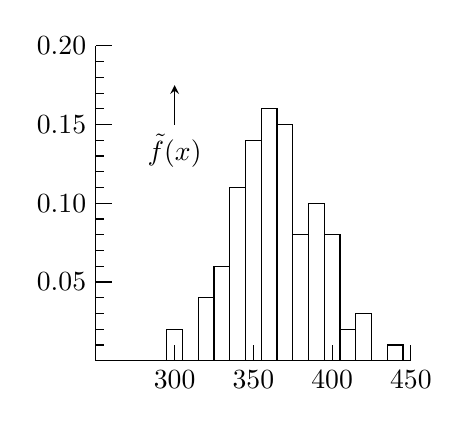
\begin{tikzpicture}
\pgfmathsetmacro{\w}{0.1}
\draw(0,0)--(4,0);
\draw(0,0)--(0,4);
\foreach \y/\ys in {1/0.05,2/0.10,3/0.15,4/0.20}{\draw(0,\y)node[left]{$\ys$}--++(0.2,0);}
\foreach \y in {0.2,0.4,0.6,0.8}{\draw(0,0+\y)--++(0.1,0)  (0,1+\y)--++(0.1,0) (0,2+\y)--++(0.1,0) (0,3+\y)--++(0.1,0);}
\foreach \x/\xs in {1/300,2/350,3/400,4/450}{\draw(\x,0)node[below]{$\xs$}--++(0,0.2);}
\draw(1-\w,0)--++(0,0.4)--++(2*\w,0)--++(0,-0.4);
\draw(1.4-\w,0)--++(0,0.8)--++(2*\w,0);
\draw(1.6-\w,0)--++(0,1.2)--++(2*\w,0);
\draw(1.8-\w,0)--++(0,2.2)--++(2*\w,0);
\draw(2-\w,0)--++(0,2.8)--++(2*\w,0);
\draw(2.2-\w,0)--++(0,3.2)--++(2*\w,0)--++(0,-0.2);
\draw(2.4-\w,0)--++(0,3)--++(2*\w,0)--++(0,-1.4);
\draw(2.6-\w,0)--++(0,1.6)--++(2*\w,0);
\draw(2.8-\w,0)--++(0,2)--++(2*\w,0)--++(0,-0.4);
\draw(3-\w,0)--++(0,1.6)--++(2*\w,0)--++(0,-1.2);
\draw(3.2-\w,0)--++(0,0.4)--++(2*\w,0);
\draw(3.4-\w,0)--++(0,0.6)--++(2*\w,0)--++(0,-0.6);
\draw(3.8-\w,0) rectangle ++(2*\w,0.2);
\draw[-stealth](1,3)node[below]{$\tilde{f}(x)$}--++(0,0.5);
\end{tikzpicture}
\caption*{(پ) تعددی مستطیلی ترسیم}
\end{subfigure}%
\begin{subfigure}{0.5\textwidth}
\centering
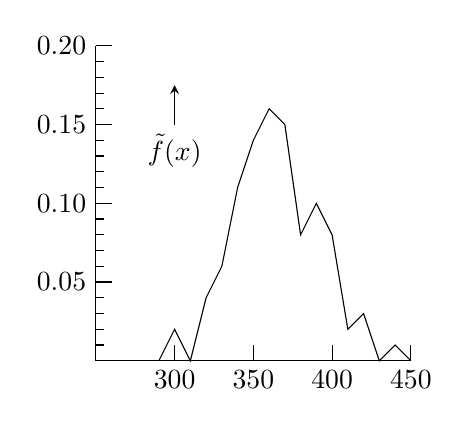
\begin{tikzpicture}
\pgfmathsetmacro{\w}{0.1}
\draw(0,0)--(4,0);
\draw(0,0)--(0,4);
\foreach \y/\ys in {1/0.05,2/0.10,3/0.15,4/0.20}{\draw(0,\y)node[left]{$\ys$}--++(0.2,0);}
\foreach \y in {0.2,0.4,0.6,0.8}{\draw(0,0+\y)--++(0.1,0)  (0,1+\y)--++(0.1,0) (0,2+\y)--++(0.1,0) (0,3+\y)--++(0.1,0);}
\foreach \x/\xs in {1/300,2/350,3/400,4/450}{\draw(\x,0)node[below]{$\xs$}--++(0,0.2);}
\draw(0.8,0)--(1,0.4)--(1.2,0)--(1.4,0.8)--(1.6,1.2)--(1.8,2.2)--(2,2.8)--(2.2,3.2)--(2.4,3)--(2.6,1.6)--(2.8,2)--(3,1.6)--(3.2,0.4)--(3.4,0.6)--(3.6,0)--(3.8,0.2)--(4,0);
\draw[-stealth](1,3)node[below]{$\tilde{f}(x)$}--++(0,0.5);
\end{tikzpicture}
\caption*{(ت) تعددی کثیر الاضلاع ترسیم}
\end{subfigure}%
\caption{ترسیم برائے جدول \حوالہ{جدول_شماریات_تعددی_تقسیم_الف}}
\label{شکل_شماریات_تعددی_ترسیم}
\end{figure}


نمونہ کا \موٹا{ترسیمی اظہار} شکل \حوالہ{شکل_شماریات_تعددی_ترسیم}-الف تا شکل \حوالہ{شکل_شماریات_تعددی_ترسیم}-ت میں دکھایا گیا ہے۔شکل \حوالہ{شکل_شماریات_تعددی_ترسیم}-پ میں ہر مستطیل کا رقبہ مطابقتی اضافی تعدد کے برابر  ہو گا لہٰذا عمودی محدد پر اضافی تعدد فی اکائی رقبہ ہو گا۔چونکہ شکل \حوالہ{شکل_شماریات_تعددی_ترسیم}-پ میں تمام مستطیل کی چوڑائی ایک جیسی ہے  لہٰذا عمودی محدد پر قیمتیں \عددی{\tilde{f}(x)} کے راست متناسب ہوں گی۔ البتہ مستطیل کو چوڑائیاں مختلف ہونے کی صورت میں ایسا نہیں ہو گا۔ شکل \حوالہ{شکل_شماریات_تعددی_ترسیم}-ت میں بھی یہی صورت حال ہو گی۔

ہم اب درج ذیل تفاعل متعارف کرتے ہیں
\begin{align*}
\tilde{F}(x)=\text{\RL{\عددی{x} اور \عددی{x} سے کم تمام قیمتوں کے اضافی تعدد کا مجموعہ}}
\end{align*}
جس کو \اصطلاح{نمونے کا مجموعی  تعددی تفاعل}\فرہنگ{تعددی!نمونے کا مجموعی تفاعل}\حاشیہب{cumulative frequency function of the sample}\فرہنگ{frequency!cumulative function of sample} یا مختصراً \اصطلاح{تقسیمی تفاعل نمونہ}\فرہنگ{تقسیمی تفاعل نمونہ}\فرہنگ{تقسیم!تقسیمی تفاعل نمونہ}\حاشیہب{sample distribution function}\فرہنگ{sample distribution function} کہتے ہیں۔شکل \حوالہ{شکل_شماریات_مجموعی_تعددی_تفاعل} میں مثال دی گئی ہے۔

\begin{figure}
\centering
\begin{subfigure}{1\textwidth}
\centering
\begin{tikzpicture}[x={2cm},y={0.5cm}]
\draw(0,4)--(0,0)--(5,0)node[right]{$x$};
\foreach \y/\ys in {2/0.1,4/0.2}{\draw(0,\y)node[left]{$\ys$}--++(0.2,0);}
\foreach \y in {1,3}{\draw(0,\y)--++(0.1,0);}
\foreach \x/\y in {1/0.2,1.4/0.8,1.6/1.2,1.8/2.2,2/2.8,2.2/3.2,2.4/3,2.6/1.6,2.8/2,3/1.6,3.2/0.4,3.4/0.6,3.8/0.2}{\draw(\x,0)--++(0,\y);}
\draw[-stealth](0.5,3)node[below]{$\tilde{f}(x)$}--++(0,0.5);
\end{tikzpicture}
\end{subfigure}
\begin{subfigure}{1\textwidth}
\centering
\begin{tikzpicture}[x={2cm},y={5cm}]
\draw(0,1)--(0,0)--(5,0)node[right]{$x$};
\foreach \y in {0.2,0.4,0.6,0.8}{\draw(0,0.5*\y)--++(0.1,0)  (0,0.5+0.5*\y)--++(0.1,0);}
\foreach \y in {0.5,1}{\draw(0,\y)node[left]{$\y$}--++(0.2,0);}
\foreach \x/\xs in {1/300,2/350,3/400,4/450}{\draw(\x,0)node[below]{$\xs$}--++(0,0.02);}
\foreach \x in {0.2,0.4,0.6,0.8} {\draw(\x,0)--++(0,0.01) (1+\x,0)--++(0,0.01)  (2+\x,0)--++(0,0.01) (3+\x,0)--++(0,0.01)  (4+\x,0)--++(0,0.01);}
\draw[-stealth](0.5,0.75)node[below]{$\tilde{F}(x)$}--++(0,0.2);
\draw(1,0)--(1,0.02)--(1.4,0.02)--(1.4,0.06)--(1.6,0.06)--(1.6,0.12)--(1.8,0.12)--(1.8,0.23)--(2,0.23)--(2,0.37)--(2.2,0.37)--(2.2,0.53)--(2.4,0.53)--(2.4,0.68)--(2.6,0.68)--(2.6,0.76)--(2.8,0.76)--(2.8,0.86)--(3,0.86)--(3,0.94)--(3.2,0.94)--(3.2,0.99)--(3.8,0.99)--(3.8,1)--(5,1);
\end{tikzpicture}
\end{subfigure}%
\caption{تعددی تفاعل \عددی{\tilde{f}(x)} اور مجموعی تعددی تفاعل \عددی{\tilde{F}(x)} برائے جدول \حوالہ{جدول_شماریات_تعددی_تقسیم_الف}}
\label{شکل_شماریات_مجموعی_تعددی_تفاعل}
\end{figure}

\عددی{\tilde{F}(x)} \ترچھا{سیڑھی تفاعل} (ٹکڑوں میں مستقل تفاعل) ہے جس میں ٹھیک ان \عددی{x}  پر جہاں \عددی{\tilde{f}(x)\ne0} ہو \عددی{\tilde{f}(x)} کے برابر چلانگ پائے جاتے ہیں۔پہلی چھلانگ نمونہ کی کم سے کم قیمت اور آخری چھلانگ نمونہ کی زیادہ سے زیادہ قیمت پر پائی جائے گی۔ آخری چھلانگ  کے بعد \عددی{\tilde{F}(x)=1} رہے گا۔

\عددی{\tilde{f}(x)} اور \عددی{\tilde{F}(x)} کا تعلق درج ذیل ہے
\begin{align}
\tilde{F}(x)=\sum_{t\le x}\tilde{f}(t)
\end{align}
جہاں \عددی{t\le x} کا مطلب  ہے کہ کسی بھی \عددی{x} کے لئے ان تمام \عددی{\tilde{f}(x)} کا مجموعہ لیا جائے گا جن کے لئے \عددی{t} کی قیمت \عددی{x} کے برابر یا \عددی{x} سے کم ہو۔

اگر کسی نمونہ میں مختلف اعداد کی تعداد بہت زیادہ ہو تب اس کا جدولی اور ترسیمی  اظہار غیر ضروری طور پر مشکل ہو گا جس کو \اصطلاح{گروہ بندی}\فرہنگ{گروہ بندی}\حاشیہب{grouping}\فرہنگ{grouping} سے آسان بنانا ممکن ہے۔آئیں گروہ بندی کے عمل کو سمجھیں۔

دیے گئے نمونہ کے لحاظ سے ہم ایسا وقفہ \عددی{I} منتخب کرتے ہیں جس میں تمام نمونی  قیمتیں شامل ہوں۔ہم \عددی{I} کو ٹکڑوں میں تقسیم کرتے ہیں جنہیں \اصطلاح{جماعتی وقفہ}\فرہنگ{جماعتی!وقفہ}\حاشیہب{class intervals}\فرہنگ{class!intervals} کہتے ہیں۔ان جماعتی وقفوں کے وسطی نقطوں کو \اصطلاح{جماعتی وسطی نقطے}\فرہنگ{جماعتی_وسطی نقطہ}\حاشیہب{class midpoints}\فرہنگ{class!midpoints} یا \اصطلاح{جماعتی نشان}\فرہنگ{جماعتی!نشان}\حاشیہب{class marks}\فرہنگ{class!marks} کہتے ہیں۔ہر جماعتی وقفہ میں پائے جانے والے نمونی قیمتیں کو \اصطلاح{طبقہ}\فرہنگ{طبقہ}\حاشیہب{class}\فرہنگ{class} کہتے ہیں۔ طبقہ  میں نمونی قیمتوں کی تعداد کو \اصطلاح{جماعتی تعدد}\فرہنگ{جماعتی!تعدد}\حاشیہب{class frequency}\فرہنگ{class!frequency} کہتے ہیں جس کو جسامت نمونہ \عددی{n} سے تقسیم کرنے سے \اصطلاح{اضافی جماعتی تعدد}\فرہنگ{جماعتی!اضافی تعدد}\حاشیہب{relative class frequency}\فرہنگ{class!relative frequency} حاصل ہو گا۔ اس تعدد \عددی{\tilde{f}(x)} کو جو جماعتی نشان کے تابع ہے  \اصطلاح{گروہ بند نمونہ کا تعددی تفاعل}\فرہنگ{تعددی! تفاعل، گروہ بند نمونہ}\حاشیہب{frequency function of the grouped sample}\فرہنگ{frequency!function of the grouped sample} کہتے ہیں۔اسی طرح  مجموعی اضافی جماعتی تعدد \عددی{\tilde{F}(x)} جو جماعتی نشان کے تابع ہے \اصطلاح{گروہ بند نمونہ کا تقسیمی تفاعل}\فرہنگ{تقسیمی!تفاعل،گروہ بند نمونہ}\فرہنگ{distribution function of the grouped sample}\حاشیہب{distribution!function of the grouped sample} کہلاتا ہے۔جدول \حوالہ{جدول_شماریات_دھاگہ_مضبوطی} اور جدول \حوالہ{جدول_شماریات_تعددی_گروہ_بند} میں مثال دیا گیا ہے۔
\begin{table}
\caption{کپاس کے سوتی دھاگے کو توڑنے کے لئے درکار قوت (نیوٹن میں)}
\label{جدول_شماریات_دھاگہ_مضبوطی}
\centering
\begin{otherlanguage}{english}
\begin{tabular}{RRRRRRRRRR}
\hline
114&118&86&107&87&94&82&81&98&84\\
120&126&98&89&114&83&94&106&96&111\\
123&110&83&118&83&96&96&74&91&81\\
102&107&103&80&109&71&96&91&86&129\\
130&104&86&121&96&96&127&94&102&87\\
\hline
\end{tabular}
\end{otherlanguage}
\end{table}

\begin{table}
\caption{تعددی جدول برائے جدول \حوالہ{جدول_شماریات_دھاگہ_مضبوطی} (گروہ بند)}
\label{جدول_شماریات_تعددی_گروہ_بند}
\centering
\begin{otherlanguage}{english}
\begin{tabular}{R|C|L|R|R|R}
\hline
\multirow{2}{*}{\text{\RL{\urdufont{جماعتی وقفہ}}}}&\text{\RL{\urdufont{جماعتی نشان}}}&\multicolumn{2}{C|}{\text{\RL{\urdufont{حتمی تعدد}}}}&\multirow{2}{*}{$\tilde{f}(x)$}&\multirow{2}{*}{$\tilde{F}(x)$}\\
\cline{3-4}
&x&\text{\RL{\urdufont{نشان شمار}}}&&&\\
\hline
65- 75&70&||&2&0.04&0.04\\
75- 85&80&&8&0.16&0.20\\
85- 95&90&&11&0.22&0.42\\
95-105&100&&12&0.24&0.66\\
105-115&110&&8&0.16&0.82\\
115-125&120&&5&0.10&0.92\\
125-135&130&&4&0.08&1.00\\
\hline
&&\text{\urdufont{مجموعہ}}&50&1.00&\\
\hline
\end{tabular}
\end{otherlanguage}
\end{table}

جماعتوں کی تعداد جتنی کم رکھی جائے، گروہ بند نمونہ کی تقسیم اتنی  سادہ ہو گی اور اتنی ہی زیادہ معلومات کھوئی جائے گی چونکہ اصل نمونی قیمتیں اب صریحاً نظر نہیں آئیں گی۔گروہ بندی کرتے وقت دھیان رکھیں کہ صرف غیر ضروری معلومات کھوئی جائے۔ گروہ بند نمونہ استعمال کرتے ہوئے مشکلات سے بچنے کی خاطر درج ذیل اصولوں کا خیال رکھیں۔
\begin{itemize}
\item
جماعتی وقفے برابر رکھیں۔
\item
جماعتی نشان یوں منتخب کریں کہ جماعتی نشان سادہ اعداد (جن میں غیر صفر ہندسوں کی تعداد کم سے کم ہو) پر واقع ہوں۔
\item
اگر نمونی قیمت \عددی{x_j} دو جماعتوں کی سرحد پر واقع ہو تب یہ قیمت اس طبقہ میں شامل کیا جائے گا جو \عددی{x_j} سے شروع ہوتا ہو۔ 
\end{itemize}

%==========================
\حصہء{سوالات}
%==============
سوال \حوالہ{سوال_شماریات_ترسیم_الف} تا سوال \حوالہ{سوال_شماریات_ترسیم_ب} میں دیے گئے نمونہ کا تعددی جدول بنائیں اور نمونہ کو تعددی نقطہ ترسیم، ڈبہ ترسیم اور مستطیل ترسیم کی صورت میں دکھائیں۔

%==================
\ابتدا{سوال}\شناخت{سوال_شماریات_ترسیم_الف}\quad مزاحمت کی قیمت اوہم \عددی{\si{\ohm}} میں۔
\begin{align*}
\begin{array}{rrrrrrrrrr}
99&100&102&101&98&103&100&102&99&101\\
100&100&99&101&100&102&99&101&98&100
\end{array}
\end{align*}

\انتہا{سوال}
%====================
\ابتدا{سوال}\شناخت{سوال_شماریات_درکار_ترسیم_ت}\quad 
\begin{align*}
\begin{array}{rrrrrrrrrrrrrrr}
6& 2& 4& 1& 2& 4& 3& 3& 2& 1& 6& 5& 6& 3& 4
\end{array}
\end{align*}

\انتہا{سوال}
%========================
\ابتدا{سوال}\شناخت{سوال_شماریات_ترسیم_پ}\quad برقی سوئچ کا سیکنڈوں میں دورانیہ ردعمل 
\begin{align*}
\begin{array}{rrrrrrrrrr}
1.3&1.4&1.1&1.5&1.4&1.3&1.2&1.4&1.5&1.3\\
1.2&1.3&1.5&1.4&1.4&1.6&1.3&1.5&1.1&1.4
\end{array}
\end{align*}
\انتہا{سوال}
%=============================
\ابتدا{سوال}\شناخت{سوال_شماریات_درکار_ترسیم_ٹ}\quad خام کوئلہ میں کوئلہ کی فی صد مقدار
\begin{align*}
\begin{array}{rrrrrrrrrr}
87&86&85&87&86&87&86&81&77&85\\
86&84&83&83&82&84&83&79&82&73
\end{array}
\end{align*}
\انتہا{سوال}
%=============================
\ابتدا{سوال}\quad چادری فولاد کی تنشی مضبوطی [\si{\kilo\gram\per\milli\meter\squared}]
\begin{align*}
\begin{array}{rrrrrrrrrrrrrrr}
44&43&41&41&44&44&43&44&42&45&43&43&44&45&46\\
42&45&41&44&44&43&44&46&41&43&45&45&42&44&44
\end{array}
\end{align*}
\انتہا{سوال}
%=============================
\ابتدا{سوال}\quad  خود کار نظام سے \عددی{100} کاغذ  کے گھٹے بنانے میں کمی بیشی
\begin{align*}
\begin{array}{rrrrrrrrrr}
0&-1&0&0&1&1&2&0&1&0
\end{array}
\end{align*}
\انتہا{سوال}
%=============================
\ابتدا{سوال}\quad  ایک ہی قسم کے گاڑیوں کا تیل کا خرچہ۔  [کلومیٹر فی لیٹر]  
\begin{align*}
\begin{array}{rrrrrr}
12& 11.5&11&12.5&11&12
\end{array}
\end{align*}
\انتہا{سوال}
%=============================
\ابتدا{سوال}\quad  خود کار نظام سے بھری گئی تھیلوں کا گرام میں وزن
\begin{align*}
\begin{array}{rrrrrrrr}
200&203&199&198&201&200&201&201
\end{array}
\end{align*}
\انتہا{سوال}
%=============================
\ابتدا{سوال}\شناخت{سوال_شماریات_ترسیم_ب}\quad  اندرون شہر چلتی ریل گاڑی کا اڈے پر ٹھیک وقت پر پہنچنے سے انحراف (منٹوں میں)\حاشیہد{امید کی جا سکتی ہے کہ ایک دن ہماری ریل گاڑیاں بھی وقت کی اتنی پابند ہوں گی۔}
\begin{align*}
\begin{array}{rrrrrrrrrr}
3&4&1&0&2&2&3&1&5&3
\end{array}
\end{align*}
\انتہا{سوال}
%=============================
\ابتدا{سوال}\شناخت{سوال_شماریات_درکار_الف}\quad
سوال \حوالہ{سوال_شماریات_ترسیم_پ} کے نمونہ کی مجموعی تعددی تفاعل کا ترسیم کھینچیں۔
\انتہا{سوال}
%===========================
\ابتدا{سوال}\quad
جدول \حوالہ{جدول_شماریات_تعددی_گروہ_بند} کے گروہ بند نمونہ کا ڈبہ ترسیم، مستطیل ترسیم اور تعددی کثیر الاضلاع ترسیم کھینچیں۔ 
\انتہا{سوال}
%======================
\ابتدا{سوال}\quad
جدول \حوالہ{جدول_شماریات_کنکریٹ_بیلن} میں جماعتی وقفوں کے جماعتی نشان \عددی{300}، \عددی{320}، \عددی{340}، \نقطے پر لیتے ہوئے مطابقتی تعددی جدول بنائیں۔اس کے مستطیل ترسیم کھینچ کا شکل \حوالہ{شکل_شماریات_تعددی_ترسیم}-پ کے ساتھ موازنہ کریں۔
\انتہا{سوال}
%===========================
\ابتدا{سوال}\quad
جدول \حوالہ{جدول_شماریات_دھاگہ_مضبوطی} میں جماعتی نشان \عددی{75}، \عددی{85}، \عددی{95}، \نقطے لے کر مطابقتی تعددی جدول بنائیں۔اس کے مستطیل ترسیم کا سوال \حوالہ{سوال_شماریات_درکار_الف} کے ترسیم سے موازنہ کریں۔  
\انتہا{سوال}
%===================
\ابتدا{سوال}\quad
\عددی{1500} تجرباتی نتائج میں سب سے کم ناپ \عددی{\SI{10.8}{\centi\meter}} اور سب سے زیادہ ناپ \عددی{\SI{11.9}{\centi\meter}} تھی۔اس مواد کی گروہ بندی لے لئے جماعتی وقفہ تجویز کریں۔
\انتہا{سوال}
%==================

\حصہ{نمونی اوسط اور نمونی تغیریت}\شناخت{حصہ_شماریات_نمونی_اوسط_نمونی_تغیریت}
تعددی تفاعل (یا تقسیمی تفاعل) نمونہ کی صحیح تصویر کشی کرتا ہے۔اس تفاعل سے ہم نمونہ کے کئی خواص کا حساب لگا سکتے ہیں مثلاً نمونی قیمتوں کی اوسط جسامت، پھیل، تشاکل، وغیرہ۔ اس حصہ میں ہم ایسے اہم ترین دو قیمتوں، نمونی اوسط اور نمونی تغیریت، پر غور کریں گے۔

نمونہ \عددی{x_1,x_2,\cdots,x_n} کی اوسط قیمت یا مختصراً \اصطلاح{نمونی اوسط}\فرہنگ{نمونی!اوسط}\فرہنگ{اوسط}\حاشیہب{sample mean}\فرہنگ{sample!mean} کو \عددی{\bar{x}} سے ظاہر کیا جاتا ہے جس کی تعریف درج ذیل کلیہ دیتی ہے۔
\begin{align}\label{مساوات_شماریات_نمونی_اوسط_الف}
\bar{x}=\frac{1}{n}\sum_{j=1}^{n}x_j=\frac{1}{n}(x_1+x_2+\cdots+x_n)
\end{align}
تمام نمونی قیمتوں کے مجموعہ کو جسامت \عددی{n} سے تقسیم کرتے ہوئے نمونی اوسط حاصل ہو گا۔ظاہر ہے کہ یہ نمونی قیمتوں کی اوسط جسامت دے گا۔

نمونہ \عددی{x_1,x_2,\cdots,x_n} کی \اصطلاح{نمونی تغیریت}\فرہنگ{نمونی!تغیریت}\فرہنگ{تغیریت}\حاشیہب{sample variance}\فرہنگ{sample!variance} کو \عددی{s^2} سے ظاہر کیا جاتا ہے جس کی تعریف درج ذیل کلیہ دیتی ہے۔
\begin{gather}
\begin{aligned}\label{مساوات_شماریات_نمونی_اوسط_ب}
s^2&=\frac{1}{n-1}\sum_{j=1}^{n}(x_j-\bar{x})^2\\
&=\frac{1}{n-1}[(x_1-\bar{x})^2+(x_2-\bar{x})^2+\cdots +(x_n-\bar{x})^2]
\end{aligned}
\end{gather}
نمونی اوسط \عددی{\bar{x}} سے نمونی قیمتوں کے انحراف کے مربعوں کو \عددی{n-1} سے تقسیم کرتے ہوئے نمونی تغیریت حاصل ہو گی۔یہ نمونی قیمتوں کی انحراف یا پھیل کی ناپ ہے۔نمونی تغیریت غیر منفی عدد ہو گا۔ نمونی تغیریت \عددی{s^2} کا مثبت جذر \اصطلاح{معیاری انحراف}\فرہنگ{معیاری انحراف}\حاشیہب{standard deviation}\فرہنگ{standard deviation} کہلاتا ہے جس کو \عددی{s} سے ظاہر کیا جاتا ہے۔

%=================
\ابتدا{مثال}\شناخت{مثال_شماریات_اوسط}\quad \موٹا{نمونی اوسط اور نمونی تغیریت}\\
بے ترتیب منتخب کیے گئے کیلوں کی  (سنٹی میٹروں میں) لمبائیاں درج ذیل ہیں۔
\begin{align*}
\begin{array}{cccccccccc}
0.80&0.81&0.81&0.82&0.81&0.82&0.80&0.82&0.81&0.81
\end{array}
\end{align*}
مساوات \حوالہ{مساوات_شماریات_نمونی_اوسط_الف} سے نمونی اوسط
\begin{align*}
\bar{x}=\frac{1}{10}(0.80+0.81+0.81+0.82+\cdots+0.81)=\SI{0.811}{\centi\meter}
\end{align*}
اور مساوات \حوالہ{مساوات_شماریات_نمونی_اوسط_ب} سے نمونی تغیریت
\begin{align*}
s^2=\frac{1}{9}[(0.80-0.811)^2+\cdots+(0.81-0.811)^2]=\SI{0.000054}{\centi\meter\squared}
\end{align*}
ہے۔ایک جیسی نمونی قیمتوں کو اکٹھا لکھنے سے حساب نسبتاً آسان بنایا جا سکتا ہے جیسے
\begin{align*}
\bar{x}=\frac{1}{10}(2\cdot 0.80+5\cdot 0.81+3\cdot 0.82)=\SI{0.811}{\centi\meter}
\end{align*} 
جہاں قوسین میں تین مختلف نمونی قیمتوں \عددی{x_1=0.80}، \عددی{x_2=0.81} اور \عددی{x_3=0.82} کو ان کی تعدد سے ضرب دیا گیا ہے۔اسی طرح
\begin{align*}
s^2=\frac{1}{9}[(2(0.800-0.811)^2+5(0.810-0.811)^2+3(0.820-0.811)^2]=\num{0.000054}
\end{align*}
ہو گا۔
\انتہا{مثال}
%=========================
اس مثال میں ہم نے \عددی{\bar{x}} اور \عددی{s^2} کو نمونہ کے تعددی تفاعل \عددی{\tilde{f}(x)} کی مدد سے حاصل کرنا دیکھا۔اگر ایک نمونہ میں ٹھیک \عددی{m} مختلف اعدادی قیمتیں 
\begin{align*}
x_1, x_2,\cdots, x_m
\end{align*}
پائی جاتی ہوں جن کے مطابقتی اضافی تعدد
\begin{align*}
\tilde{f}(x_1),\tilde{f}(x_2),\cdots,\tilde{f}(x_m)
\end{align*}
ہوں تب حساب کے لئے درکار تعدد درج ذیل ہوں گے
\begin{align*}
n\tilde{f}(x_1),n\tilde{f}(x_2),\cdots,n\tilde{f}(x_m)
\end{align*}
جنہیں استعمال کرتے ہوئے مساوات \حوالہ{مساوات_شماریات_نمونی_اوسط_الف} اور مساوات \حوالہ{مساوات_شماریات_نمونی_اوسط_ب} سے
\begin{align}\label{مساوات_شماریات_نمونی_اوسط_پ}
\bar{x}=\frac{1}{n}\sum_{j=1}^{m}x_jn\tilde{f}(x_j)
\end{align}
اور
\begin{align}\label{مساوات_شماریات_نمونی_اوسط_ت}
s^2=\frac{1}{n-1}\sum_{j=1}^{m} (x_j-\bar{x})^2n\tilde{f}(x_j)
\end{align}
حاصل ہو گا۔ دھیان رہے کہ مساوات \حوالہ{مساوات_شماریات_نمونی_اوسط_الف} اور مساوات \حوالہ{مساوات_شماریات_نمونی_اوسط_ب} میں ہم تمام نمونی قیمتوں پر مجموعہ لیتے ہیں جبکہ مساوات \حوالہ{مساوات_شماریات_نمونی_اوسط_پ} اور مساوات \حوالہ{مساوات_شماریات_نمونی_اوسط_ت} میں ہم اعدادی طور مختلف نمونی قیمتوں پر مجموعہ حاصل کرتے ہیں۔حتمی تعدد \عددی{n\tilde{f}(x_j)} عدد صحیح ہوں گے جبکہ اضافی تعدد \عددی{\tilde{f}(x_j)} عموماً غیر عدد صحیح ہوں گے۔

چونکہ \عددی{x_j-\bar{x}} کی حتمی قیمت نمونی اوسط کی نسبت بہت کم ہو سکتی ہے لہٰذا \عددی{s^2} کے مذکورہ بالا کلیات کی استعمال سے (خود کار حساب میں) ملحوظ ہندسے ضائع ہوں گے۔ہم \عددی{s^2} کا ایک ایسا کلیہ اخذ کرتے ہیں جو ان مشکلات سے دو چار نہ ہو۔ہم  مساوات \حوالہ{مساوات_شماریات_نمونی_اوسط_ب} میں
\begin{align*}
(x_j-\bar{x})^2=x_j^2-2x_j\bar{x}+\bar{x}^2
\end{align*}
پر کرتے ہوئے تین مجموعے 
\begin{align*}
\sum(x_j-\bar{x})^2=\sum x_j^2-2\bar{x}\sum x_j+\sum \bar{x}^2
\end{align*}
حاصل کرتے ہیں جہاں آخری مجموعہ \عددی{n\bar{x}^2} کے برابر ہے۔ مساوات \حوالہ{مساوات_شماریات_نمونی_اوسط_الف} سے \عددی{\bar{x}} کی قیمت پر کرتے ہوئے
\begin{align*}
-2\bar{x}\sum x_j=-\frac{2}{n}(\sum x_j)^2 \quad \text{اور}\quad n\bar{x}^2=\frac{1}{n}(\sum x_j)^2
\end{align*}
لکھا جا سکتا ہے جنہیں استعمال کرتے ہوئے
\begin{align}\label{مساوات_شماریات_نمونی_اوسط_ٹ}
s^2=\frac{1}{n-1}\big[\sum_{j=1}^{n}x_j^2-\frac{1}{n}\big(\sum_{j=1}^{n}x_j\big)^2\big]
\end{align}
حاصل ہو گا۔ اسی طرح  مساوات \حوالہ{مساوات_شماریات_نمونی_اوسط_ت} کو تبدیل کرتے ہوئے
\begin{align}\label{مساوات_شماریات_نمونی_اوسط_ث}
s^2=\frac{1}{n-1}\big[\sum_{j=1}^{m} x_j^2n\tilde{f}(x_j)-\frac{1}{n}\big(\sum_{j=1}^{m}x_jn\tilde{f}(x_j)\big)^2\big]
\end{align}
حاصل کیا جا سکتا ہے۔

مثال کے طور پر مثال \حوالہ{مثال_شماریات_اوسط} میں مساوات \حوالہ{مساوات_شماریات_نمونی_اوسط_پ} اور مساوات \حوالہ{مساوات_شماریات_نمونی_اوسط_ث} (جدول \حوالہ{جدول_شماریات_اوسط_تغیریت}) سے پہلے کی طرح \عددی{\bar{x}=\tfrac{8.11}{10}=0.811} اور  
\begin{align*}
s^2=\frac{1}{9}\big(6.5777-\frac{8.11^2}{10}\big)=\frac{\num{0.00049}}{9}=\num{0.000054}
\end{align*}
حاصل ہوتے ہیں۔
\begin{table}
\caption{اوسط اور تغیریت کا حساب برائے مثال \حوالہ{مثال_شماریات_اوسط}}
\label{جدول_شماریات_اوسط_تغیریت}
\centering
\begin{otherlanguage}{english}
\begin{tabular}{C|C|C|C|C}
\hline
\Tstrut
x_j&10\tilde{f}(x_j)&x_j\cdot 10 \tilde{f}(x_j)&x_j^2&x_j^2\cdot 10 \tilde{f}(x_j)\\
\hline
0.80&2&1.60&0.6400&1.2800\\
0.81&5&4.05&0.6561&3.2805\\
0.82&3&2.46&0.6724&2.0172\\
\hline
\end{tabular}
\end{otherlanguage}
\end{table}

%=======================
\حصہء{سوالات}
%=====================
\ابتدا{سوال}\quad
گزشتہ حصے کی سوال \حوالہ{سوال_شماریات_درکار_ترسیم_ت} کے لئے نمونی اوسط اور نمونی تغیریت تلاش کریں۔\\
جواب:\quad
$\bar{x}=3.47,\,\, s^2=2.98$
\انتہا{سوال}
%=======================
\ابتدا{سوال}\quad
گزشتہ حصے کی سوال \حوالہ{سوال_شماریات_درکار_ترسیم_ٹ} کے لئے نمونی اوسط اور نمونی تغیریت تلاش کریں۔\\
جواب:\quad
$\bar{x}=84,\,\,s^2=\tfrac{1251}{95}$
\انتہا{سوال}
%=======================
\ابتدا{سوال}\quad
نمونہ \عددی{2,1,4,5} کا مستطیل ترسیم کھینچیں۔ترسیم کو دیکھ کر \عددی{\bar{x}} اور \عددی{s} کی قیمتوں کا اندازہ لگائیں۔\عددی{\bar{x}}، \عددی{s^2} اور \عددی{s} کی قیمتوں کا حساب لگائیں۔\\
جواب:\quad
$\bar{x}=3,\,\, s^2=3.3,\,\, s=1.817$
\انتہا{سوال}
%=====================
\ابتدا{سوال}\quad
دکھائیں کہ کم سے کم اور زیادہ سے زیادہ نمونی قیمتوں کے بیچ \عددی{\bar{x}} ہو گا۔
\انتہا{سوال}
%===========================
\ابتدا{سوال}\quad \موٹا{نمونہ کا }\\
نمونہ میں سب سے بڑی قیمت اور سب سے چھوٹی قیمت کے فرق کو نمونہ کا \اصطلاح{}\فرہنگ{}\حاشیہب{range}\فرہنگ{range} کہتے ہیں۔مثال \حوالہ{مثال_شماریات_اوسط} میں دیے گئے نمونہ کا  تلاش کریں۔\\
جواب:\quad
$0.02$
\انتہا{سوال}
%==========================
\ابتدا{سوال}\quad \موٹا{صدویہ، وسطانیہ}\\
نمونہ کی \عددی{p} ویں \اصطلاح{صدویہ}\فرہنگ{صدویہ}\حاشیہب{percentile}\فرہنگ{percentile} سے مراد ایسا عدد \عددی{Q_p} ہے کہ کم از کم \عددی{p\,\si{\percent}} نمونی قیمتیں \عددی{Q_p} سے کم یا اس کے برابر ہوں اور ساتھ ہی \عددی{(100-p)\,\si{\percent}} نمونی قیمتیں اس سے زیادہ یا اس کے برابر ہوں۔اگر ایک سے زیادہ ایسا عدد پایا جاتا ہو (جس صورت میں ان اعداد کا وقفہ پایا جائے گا) تب \عددی{p} ویں صدویہ سے مراد ان اعداد کا اوسط (یعنی وقفے  کا وسطی نقطہ) ہو گا۔بالخصوص \عددی{Q_{50}} کو \اصطلاح{وسطانیہ}\فرہنگ{وسطانیہ}\حاشیہب{median}\فرہنگ{median} کہتے ہیں جس کو \عددی{\tilde{x}} سے ظاہر کیا جاتا ہے۔وسطانیہ کو \اصطلاح{نصف چوتھائی}\فرہنگ{چوتھائی!نصف}\حاشیہب{middle quartile}\فرہنگ{quartile!middle} بھی کہتے ہیں۔جدول \حوالہ{جدول_شماریات_تعددی_تقسیم_الف} کے نمونہ  کا وسطانیہ \عددی{\tilde{x}} تلاش کریں۔\\
جواب:\quad
$360$
\انتہا{سوال}
%==========================
\ابتدا{سوال}\شناخت{سوال_شماریات_چوتھائی_الف}\quad 
نمونہ کی \عددی{Q_{25}} اور \عددی{Q_{75}} صدویہ کو بالترتیب \اصطلاح{نچلی چوتھائی}\فرہنگ{چوتھائی!نچلی}\حاشیہب{lower quartile}\فرہنگ{quartile!lower} اور \اصطلاح{بالائی چوتھائی}\فرہنگ{چوتھائی!بالائی}\حاشیہب{upper quartile}\فرہنگ{quartile!upper} کہتے ہیں جبکہ \عددی{Q_{75}-Q_{25}} جو پھیل کی ناپ ہے کو \اصطلاح{چوتھائی }\فرہنگ{چوتھائی!}\حاشیہب{interquartile range}\فرہنگ{quartile!interquartile range} کہتے ہیں۔جدول \حوالہ{جدول_شماریات_تعددی_تقسیم_الف} کے نمونہ  کا کی \عددی{Q_{25}}، \عددی{Q_{75}} اور \عددی{Q_{75}-Q_{25}} تلاش کریں۔\\
جواب:\quad
$350,\,\,380,\,\,30$
\انتہا{سوال}
%=============================
\ابتدا{سوال}\quad
جدول \حوالہ{جدول_شماریات_دھاگہ_مضبوطی} کے لئے سوال \حوالہ{سوال_شماریات_چوتھائی_الف} کو حل کریں۔\\
جواب:\quad
$\tfrac{345}{4},\,\,\tfrac{439}{4},\,\,\tfrac{47}{2}$
\انتہا{سوال}
%=========================
\ابتدا{سوال}\quad \موٹا{عادہ}\\
نمونہ میں سب سے زیادہ بار آنے والی قیمت کو نمونہ کی \اصطلاح{عادہ}\فرہنگ{عادہ}\حاشیہب{mode}\فرہنگ{mode} کہتے ہیں۔یہ سب سے عام قدر ہوتی ہے۔درج ذیل نمونہ کی اوسط، وسطانیہ اور عادہ تلاش کریں۔ ان پر تبصرہ کریں۔
\begin{align*}
\begin{array}{L|CCC}
\text{\RL{\urdufont{قیمت}}}&100&1000&\num{1000000}\\
\hline
\text{\RL{\urdufont{تعدد}}}&100&90&20
\end{array}
\end{align*}
جواب:\quad
$\text{اوسط}=\num{10000},\,\, \text{وسطانیہ}=1000,\,\,\text{عادہ}=100$
\انتہا{سوال}
%===========================
\ابتدا{سوال}\شناخت{سوال_شماریات_مبدا_کام}\quad \موٹا{مبدا کام}\\
اگر \عددی{x_j=x^*_j+c} ہو جہاں  \عددی{j=1,\cdots,n} اور \عددی{c} کوئی مستقل ہو تب دکھائیں کہ
\begin{align*}
\bar{x}=c+\bar{x}^*,\quad \big(\bar{x}^*=\frac{1}{n}\sum_{j=1}^{n}x_j^*\big)\quad  \text{اور} \quad \quad s^2=s^{*2}
\end{align*}
ہوں گے جہاں \عددی{x_j^*} قیمتوں  کی تغیریت \عددی{s^{*2}} ہے۔(عملی استعمال میں \عددی{c} یوں منتخب کیا جاتا ہے کہ \عددی{x_j^*} کی حتمی قیمتیں چھوٹی ہوں۔جیومیٹریائی طور پر یہ مبدا کی تبدیلی کے مترادف ہے لہٰذا اس کو \ترچھا{ترکیب مبدا کام}\فرہنگ{ترکیب!مبدا کام}\حاشیہب{method of working origin}\فرہنگ{method!of working origin} کہتے ہیں۔)  
\انتہا{سوال}
%=========================
\ابتدا{سوال}\quad
ترکیب مبدا کام کو مثال \حوالہ{مثال_شماریات_اوسط} کے نمونہ پر لاگو کریں۔
\انتہا{سوال}
%====================
\ابتدا{سوال}\quad \موٹا{مکمل رمز نویسی}\\
اگر \عددی{x_j=c_1x_j^*+c_2} ہو جہاں \عددی{j=1,\cdots,n} جبکہ \عددی{c_1} اور \عددی{c_2} مستقل ہیں تب دکھائیں کہ
\begin{align*}
\bar{x}=c_1\bar{x}^*+c_2,\quad s^2=c_1^2s^{*2}
\end{align*}
ہوں گے جہاں \عددی{\bar{x}^*} اور \عددی{s^{*2}} کی معنی سوال \حوالہ{سوال_شماریات_مبدا_کام} میں پیش کی گئی ہیں۔اس کو \اصطلاح{ترکیب مکمل رمز نویسی}\فرہنگ{ترکیب!مکمل رمز نویسی}\حاشیہب{method of full coding}\فرہنگ{method!of full coding} کہتے ہیں۔(اس ترکیب سے قلم و کاغذ استعمال کرتے ہوئے نتائج کی جلد جانچ پڑتال کی جا سکتی ہے۔)
\انتہا{سوال}
%======================
\ابتدا{سوال}\quad
اس ترکیب کو مثال \حوالہ{مثال_شماریات_اوسط} کے نمونہ پر لاگو کریں۔
\انتہا{سوال}
%======================
\ابتدا{سوال}\quad
کسی بھی نمونہ کی گروہ بندی سے عموماً نمونی اوسط متاثر ہو گا۔دکھائیں کہ نمونی اوسط میں تبدیل \عددی{\tfrac{l}{2}} سے زیادہ نہیں ہو سکتی ہے جہاں ہر ایک جماعتی وقفہ کی لمبائی \عددی{l} ہے۔
\انتہا{سوال}
%=======================
\ابتدا{سوال}\quad
جدول \حوالہ{جدول_شماریات_دھاگہ_مضبوطی} کی غیر گروہ بند نمونہ کی گروہ بندی  جدول \حوالہ{جدول_شماریات_تعددی_گروہ_بند} میں کی گئی ہے۔دونوں مواد کی اوسط اور تغیریت تلاش کریں۔نتائج کا آپس میں موازنہ کریں۔\\
جواب:\quad
$\text{غیر گروہ بند}:\,\, \bar{x}=99.2,\,\, s^2=234.7;\quad \text{گروہ بند}:\,\, \bar{x}=99.4,\,\, s^2=254.7$
\انتہا{سوال}
%===========================

\حصہ{بلا منصوبہ تجربات، انجام، وقوعات}\شناخت{حصہ_شماریات_تجربات_انجام_وقوعات}
شماریاتی تجربات یا شماریاتی مشاہدے  سے ہمیں نمونے حاصل ہوں گے جن کی مدد سے ہم متعلقہ  آبادی کے بارے میں نتائج اخذ کرنا چاہیں گے۔ایسا کرنے سے پہلے  حسابی احتمال کی مدد سے ہمیں آبادی کے حسابی نمونے  بنانے ہوں گے۔یہ نظریہ حسابی شماریات کی بنیاد ہے جس کی گہرائی میں ہم اپنی ضرورت کے مطابق  جائیں گے۔اس حصہ میں کئی بنیادی تصورات کو متعارف کیا جائے گا۔

ایک بلا منصوبہ تجربہ یا بلا منصوبہ  مشاہدہ، جنہیں ہم مختصراً \اصطلاح{تجربہ}\فرہنگ{تجربہ}\حاشیہب{experiment}\فرہنگ{experiment} یا \اصطلاح{مشاہدہ}\فرہنگ{مشاہدہ}\حاشیہب{observation}\فرہنگ{observation} کہیں گے، سے مراد وہ عمل ہے جو درج ذیل خواص رکھتا ہو۔
\begin{itemize}
\item
اس کو طے شدہ قواعد کے تحت سرانجام دیا جاتا ہے جو عمل کو مکمل طور پر بیان کرتے ہیں۔
\item
اس  عمل کو جتنی بار چاہیں دوبارہ انجام  دیا جا سکتا ہے۔
\item
ہر مرتبہ عمل کا نتیجہ  اتفاق پر منحصر ہو گا (یعنی نتیجہ ان اثرات پر منحصر ہے جنہیں ہم قابو نہیں کر سکتے ہیں) لہٰذا قبل از وقت  یکتا طور پر نتیجہ جاننا ممکن نہیں ہو گا۔
\end{itemize} 

ایک مرتبہ تجربے کے عمل سے حاصل نتیجہ کو  اس \اصطلاح{کوشش}\فرہنگ{کوشش}\حاشیہب{trial}\فرہنگ{trial} کا  \اصطلاح{انجام}\فرہنگ{انجام}\حاشیہب{outcome}\فرہنگ{outcome} کہتے ہیں۔

اس کی مثال (کرکٹ کی کھیل کی آغاز میں) سکہ پھینکنا، \ترچھا{لوڈو}\حاشیہب{ludo} کی کھیل میں \ترچھا{پانسہ}\حاشیہد{ایک مکعب جس کی چھ سطحوں پر ایک تا چھ نقطے ہوتے ہیں۔} پھینکنا، \عددی{100} پیچ کی ڈبی سے \عددی{10} پیچوں کا انتخاب  یا مختلف حالات میں کیمیائی عمل کی  پیداوار تعین کرنا اور دیگر تجربات مثلاً  بلا منصوبہ \عددی{20} افراد کا انتخاب اور ان کا \اصطلاح{فشار خون}\فرہنگ{فشار خون}\حاشیہب{blood pressure}\فرہنگ{blood pressure} تعین کرنا یا کسی موضوع پر ان کی رائے جاننا ہیں۔

کسی تجربہ کے تمام ممکنہ انجام کے سلسلہ کو اس تجربہ کی \اصطلاح{نمونی فضا}\فرہنگ{نمونی!فضا}\حاشیہب{sample space}\فرہنگ{sample!space} کہتے ہیں جس کو \عددی{S} سے ظاہر کیا جائے گا۔ہر ایک انجام کو \عددی{S} کا \اصطلاح{رکن}\فرہنگ{رکن}\حاشیہب{element}\فرہنگ{element} یا \اصطلاح{نقطہ}\فرہنگ{نقطہ}\حاشیہب{point}\فرہنگ{point} کہتے ہیں۔متناہی تعداد کے ارکان پر مشتمل سلسلہ \اصطلاح{متناہی} جبکہ لامتناہی تعداد کے ارکان پر مشتمل سلسلہ \اصطلاح{لامتناہی} کہلائے گا۔ 

مثال کے طور پر پانسہ پھینکنے کے بلا منصوبہ تجربہ کے ساتھ درج ذیل نمونی سلسلہ منسلک کیا جا سکتا ہے، 
\begin{align*}
S=\{1,2,3,4,5,6\}
\end{align*}
چونکہ پانسہ پھینکنے کے بعد (چھ ممکنات میں سے) کسی ایک رخ رکے گا۔

صنعتی پیداوار سے ہم  ایک رکن نکال کر دیکھ سکتے ہیں کہ آیا وہ بے عیب یا عیب دار ہے۔یوں \عددی{S} دو ارکان \عددی{D} (عیب دار)  اور \عددی{N} (بے عیب)  پر مشتمل ہو گا جنہیں اعداد مثلاً \عددی{0} (عیب دار) اور \عددی{1} (بے عیب) سے بھی ظاہر کیا جا سکتا ہے۔اب اگر ہم ایک سے زیادہ اقسام کے عیب میں تمیز کریں تب نمونی فضا دو سے زائد نقطوں پر مشتمل ہو گا۔

کپاس کی مضبوطی کے تجربہ (جدول \حوالہ{جدول_شماریات_دھاگہ_مضبوطی}) میں نمونی فضا لامتناہی ہو گا چونکہ دھاگہ توڑنے کے لئے درکار قوت کسی مخصوص  میں کوئی بھی مثبت قیمت ہو سکتی ہے۔

عملی مسائل میں ہمیں انفرادی انجام سے زیادہ دلچسپی نہیں ہو گی بلکہ ہم صرف اتنا جاننا چاہیں گے کہ آیا اس کا کسی مخصوص سلسلہ انجام سے تعلق ہے (یا نہیں ہے)۔ظاہر ہے کہ ایسا ہر سلسلہ \عددی{A} پوری نمونی فضا \عددی{S} کا ذیلی سلسلہ  ہو گا۔اس کو \اصطلاح{وقوعہ}\فرہنگ{وقوعہ}\حاشیہب{event}\فرہنگ{event} کہتے ہیں۔ 

چونکہ کوئی بھی انجام \عددی{S} کا ذیلی سلسلہ ہو گا لہٰذا یہ ایک مخصوص قسم کا وقوعہ ہو گا جس کو \ترچھا{بنیادی وقوعہ}\فرہنگ{وقوعہ!بنیادی} کہتے ہیں۔اسی طرح پوری فضا \عددی{S} بھی ایک مخصوص وقوعہ ہے۔

%=====================
\ابتدا{مثال}\شناخت{مثال_شماریات_نلکے}\quad
پانچ پانی کے نلکوں (جنہیں ایک تا پانچ سے ظاہر کیا جاتا ہے) میں سے دو نلکے منتخب کیے جاتے ہیں۔نمونی فضا درج ذیل دس ممکنہ انجام پر مشتمل ہو گی۔
\begin{align*}
1,2\quad 1,3\quad 1,4\quad 1,5\quad 2,3\quad 2,4\quad 2,5\quad 3,4\quad 3,5\quad 4,5
\end{align*}
اب اگر ہم عیب دار نلکوں میں دلچسپی رکھتے ہوں تب ہمیں درج ذیل تین انجاموں میں فرق کرنا ہو گا۔
\begin{align*}
A:\text{\RL{کوئی بھی عیب دار نہیں ہے}},\quad B:\text{\RL{ایک عیب دار ہے}},\quad C:\text{\RL{دونوں عیب دار ہیں}}
\end{align*}
فرض کریں کہ نلکوں میں \عددی{1,2,3} عیب دار ہیں تب درج ذیل ہو گا۔
\begin{align*}
\text{\RL{منتخب کرنے سے \عددی{A} ہو گا}}\quad &4,5,\\
\text{\RL{منتخب کرنے سے \عددی{B} ہو گا}}\quad &1,4\quad 1,5\quad 2,4\quad 2,5\quad 3,4\quad 3,5\\
\text{\RL{منتخب کرنے سے \عددی{C} ہو گا}}\quad &1,2\quad 1,3\quad 2,3
\end{align*} 
\انتہا{مثال}
%==========================

نمونی فضا \عددی{S} اور تجربہ کے انجام کو \اصطلاح{وین اشکال}\فرہنگ{وین اشکال}\حاشیہب{Venn diagram}\فرہنگ{Venn diagram} سے ظاہر کیا جا سکتا ہے۔ فرض کریں کہ  شکل \حوالہ{شکل_شماریاتی_وین_شکل_الف} میں چکور کے اندر نقطوں کا سلسلہ \عددی{S} کو ظاہر کرتے ہے۔تب مستطیل کے اندر بند منحنی کا اندرون کسی وقوعہ کو ظاہر کرے گا جس کو ہم \عددی{E}  سے ظاہر کرتے ہیں۔ ان تمام ارکان (انجاموں) کا سلسلہ جو \عددی{E} میں شامل نہیں ہیں کو \عددی{S} میں \عددی{E} کا متمم کہتے ہیں جس کو \عددی{E^c}\حاشیہد{یا \عددی{\bar{E}} سے ظاہر کیا جاتا ہے جس کو ہم استعمال نہیں کریں گے چونکہ اس کو کسی دوسرے مقصد (بندش سلسلہ) کے لئے مختص کیا گیا ہے۔} سے ظاہر کیا گیا ہے۔  
\begin{figure}
\centering
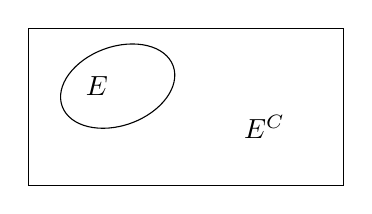
\begin{tikzpicture}
\draw(0,0) rectangle (4,2);
\draw[rotate=20](1.5,0.8)node[left]{$E$} circle (0.75cm and 0.5cm);
\draw(3,0.75)node[]{$E^C$};
\end{tikzpicture}
\caption{وین شکل میں نمونی سلسلہ \عددی{S} اور وقوعات \عددی{E} اور \عددی{E^C} دکھائے گئے ہیں}
\label{شکل_شماریاتی_وین_شکل_الف}
\end{figure}

مثال کے طور پر پانسہ پھینکنے کے تجربہ میں 
\begin{align*}
E:\quad \text{\RL{جب جفت عدد حاصل ہو}}
\end{align*}
کا متمم
\begin{align*}
E^C:\quad \text{\RL{جب طاق عدد حاصل ہو}}
\end{align*}
ہو گا۔ایسا وقوعہ جس میں کوئی انجام نہ پایا جاتا ہو کو \ترچھا{خالی وقوعہ}\فرہنگ{وقوعہ!خالی}\حاشیہب{empty event}\فرہنگ{event!empty} یا \اصطلاح{نا ممکن وقوعہ}\فرہنگ{وقوعہ!نا ممکن}\حاشیہب{impossible event}\فرہنگ{event!impossible} کہتے ہیں جس کو \عددی{\varnothing} سے ظاہر کیا جاتا ہے۔

فرض کریں کہ کسی تجربہ میں \عددی{A} اور \عددی{B} کوئی دو وقوعات ہیں۔تب  وہ وقوعہ جو \عددی{S} میں ان تمام ارکان پر مشتمل ہو جو \عددی{A} یا \عددی{B} یا دونوں میں پائے جاتے ہوں کو \عددی{A} اور \عددی{B} کا  \اصطلاح{اشتراک}\فرہنگ{اشتراک}\حاشیہب{union}\فرہنگ{union} کہلاتا ہے جس کو درج ذیل سے ظاہر کیا جاتا ہے۔
\begin{align*}
A\cup B
\end{align*} 
وہ وقوعہ جو \عددی{S} میں ان تمام ارکان پر مشتمل ہو جو \عددی{A} اور \عددی{B} دونوں میں پائے جاتے ہوں کو \عددی{A} اور \عددی{B} کا \اصطلاح{تقاطع}\فرہنگ{تقاطع}\حاشیہب{intersection}\فرہنگ{intersection} کہلاتا ہے جس کو درج ذیل سے ظاہر کیا جاتا ہے۔شکل \حوالہ{شکل_شماریات_وین_شکل_اشتراک_تقاطع} میں اشتراک اور تقاطع کو وین شکل پر دکھایا گیا ہے۔
\begin{align*}
A\cap B
\end{align*} 
%=================
\begin{figure}
\centering
\begin{subfigure}{0.5\textwidth}
\centering
\begin{tikzpicture}
\def\firstCircle{(0.75,1.75) circle (0.75cm and 0.5cm)};
\def\secondCircle{(1.5,1.5) circle (0.75cm and 0.5cm)}
%
\begin{scope}[even odd rule]
\clip  (0,0) rectangle (3,2) [rotate=-20] \firstCircle  ;
\fill[lgray,rotate=-20] \secondCircle;
\end{scope}
\fill[lgray,rotate=-20]\firstCircle;
\draw[rotate=-20](0.75,1.75)node[left]{$A$} circle (0.75cm and 0.5cm);
\draw[rotate=-20](1.5,1.5)node[right]{$B$} circle (0.75cm and 0.5cm);
\draw(0,0)node[above right]{$S$} rectangle (3,2);
\end{tikzpicture}
\caption*{(الف) اشتراک \عددی{A \cup B}}
\end{subfigure}%
\begin{subfigure}{0.5\textwidth}
\centering
\begin{tikzpicture}
\def\firstCircle {(0.75,1.75) circle (0.75cm and 0.5cm)};
\def\secondCircle{(1.5,1.5) circle (0.75cm and 0.5cm)}
\begin{scope}
\clip[rotate=-20] \firstCircle;
\fill[lgray,rotate=-20] \secondCircle;
\end{scope}
\draw[rotate=-20]\firstCircle node[left]{$A$};
\draw[rotate=-20]\secondCircle node[right]{$B$};
\draw(0,0)node[above right]{$S$} rectangle (3,2);
\end{tikzpicture}
\caption*{(ب) تقاطع \عددی{A\cap B}}
\end{subfigure}%
\caption{نمونی فضا \عددی{S} میں دو وقوعات \عددی{A} ، \عددی{B} اور (گہری سیاہی میں) ان کی اشتراک اور تقاطع کی وین شکل}
\label{شکل_شماریات_وین_شکل_اشتراک_تقاطع}
\end{figure}

اگر \عددی{A} اور \عددی{B} میں کوئی وقوعہ مشترک نہ ہو تب  \عددی{A\cup B=\varnothing} ہو گا اور ہم کہیں گے کہ \عددی{A} اور \عددی{B} \اصطلاح{بے ربط وقوع}\فرہنگ{وقوعہ!بلا شرکت}\حاشیہب{disjoint events}\فرہنگ{event!disjoint}  یا \اصطلاح{باہمی بلا شرکت وقوعہ}\فرہنگ{وقوعہ!باہمی بلا شرکت}\حاشیہب{mutually exclusive events}\فرہنگ{event!mutually exclusive} ہیں۔ 

مثال کے طور پر مثال \حوالہ{مثال_شماریات_نلکے} میں \عددی{B\cap C=\varnothing} ہے  جبکہ \عددی{B \cup C} ایک یا دو عیب دار نلکیاں ہیں۔

%==================
\ابتدا{مثال}\شناخت{مثال_شماریات_وین_پانسہ}\quad
پانسہ پھینکنے کے ایک تجربہ میں درج ذیل وقوعہ 
\begin{align*}
&A: \text{\RL{سے چھوٹا عدد نہ ہو}}\,4\\
&B:\text{سے قابل تقسیم عدد ہو}\,\, 3
\end{align*}
کا اشتراک \عددی{A\cup B=\{3,4,5,6\}} اور تقاطع \عددی{A\cap B=\{6\}} ہو گا (شکل \حوالہ{شکل_مثال_شماریات_وین_پانسہ})۔
\begin{figure}
\centering
\begin{tikzpicture}
\draw(0,0) circle (1.5cm and 0.6cm);
\draw[stealth-](-1,0)node[ocirc]{}node[below]{$4$} (0,0) node[ocirc]{}node[below]{$5$} (1,0)node[ocirc]{}node[below]{$6$}++(0.05,0.05) to [out=45,in=180]++(0.75,0.5)node[right]{$A\cap B$};
\draw(1,0.5) circle (0.4cm and 1cm);
\draw(1,1)node[ocirc]{}node[above]{$3$};
\draw(0,1)node[ocirc]{}node[above]{$2$};
\draw(-1,1)node[ocirc]{}node[above]{$1$};
\draw[stealth-](0,0)++(135:1.5cm and 0.6cm) to [out=135,in=0]++(-0.5,0.5)node[left]{$A$};
\draw[stealth-](1,0.5)++(35:0.4cm and 1cm) to [out=35,in=180]++(0.3,0.3)node[right]{$B$};
\draw[dashed]([shift={(90:1.7cm and 0.8cm)}]0,0) arc (90:360:1.7cm and 0.8cm);
\draw[dashed] ([shift={(0:0.6cm and 1.2cm)}]1,0.5) arc (0:160:0.6cm and 1.2cm)coordinate(kD);
\draw[dashed] (1,0.5)++(0:0.6cm and 1.2cm) to [out=-90,in=90] (1.7cm,0);
\draw[dashed] (90:1.7cm and 0.8cm) to [out=0,in=-100] (kD);
\draw[stealth-] (170:1.7cm and 0.8cm) to [out=160,in=0]++(-0.3,0.2)node[left]{$A\cup B$};
\end{tikzpicture}
\caption{وین شکل برائے مثال \حوالہ{مثال_شماریات_وین_پانسہ}}
\label{شکل_مثال_شماریات_وین_پانسہ}
\end{figure}
\انتہا{مثال}
%========================

اگر وقوعہ \عددی{A} کے تمام ارکان وقوعہ \عددی{B} میں پائے جاتے ہوں تب \عددی{A} کو \عددی{B} کا \اصطلاح{ذیلی وقوعہ}\فرہنگ{وقوعہ!ذیلی}\حاشیہب{subevent}\فرہنگ{event!subevent} کہتے ہیں جس کو درج ذیل لکھا جاتا ہے۔
\begin{align*}
A \subset B \quad \text{یا}\quad B \supset A
\end{align*}
ظاہر ہے کہ \عددی{A\subset B} کی صورت میں اگر \عددی{B} واقع پذیر ہو تب لازماً \عددی{A} بھی وقوع پذیر ہو گا۔مثال کے طور پر وقوعہ \عددی{D=\{4,6\}} پانسہ کے جفت نتائج کے وقوعہ \عددی{E=\{2,4,6\}} کا ذیلی وقوعہ ہے۔ 

فرض کریں کہ نمونی فضا \عددی{S} میں کئی وقوعات \عددی{A_1,\cdots,A_m} ہیں۔ تب ان \عددی{m} وقوعات میں سے ایک میں یا ایک سے زیادہ میں پائے جانے والے تمام ارکان پر مشتمل وقوعہ  ان \عددی{m} وقوعات کا \اصطلاح{اشتراک} ہو گا جس کو
\begin{align*}
\bigcup_{j=1}^{m}A_j\quad \text{\RL{یا مختصراً}}\quad A_1\cup A_2\cup\cdots \cup A_m 
\end{align*}
لکھا جاتا ہے۔ان تمام  وقوعات میں پائے جانے والے ارکان پر مشتمل وقوعہ \عددی{A_1,\cdots, A_m} کا \اصطلاح{تقاطع} ہو گا جس کو 
\begin{align*}
\bigcap_{j=1}^{m}A_j\quad \text{\RL{یا مختصراً}}\quad A_1\cap A_2\cap\cdots \cap A_m 
\end{align*}
لکھا جاتا ہے۔

زیادہ عمومی طور پر فرض کریں کہ \عددی{S} میں لامتناہی ارکان  \عددی{A_1,\cdots,A_m,\cdots} پائے جاتے ہیں۔تب \اصطلاح{اشتراک}
\begin{align*}
\bigcup_{j=1}^{\infty}A_j\quad \text{\RL{یا مختصراً}}\quad A_1\cup A_2\cup\cdots
\end{align*}
ان تمام ارکان پر مشتمل وقوعہ ہو گا جو کم سے کم کسی ایک مذکورہ بالا وقوعہ میں پائے جاتے ہوں۔اسی طرح \اصطلاح{تقاطع}
\begin{align*}
\bigcap_{j=1}^{\infty}A_j\quad \text{\RL{یا مختصراً}}\quad A_1\cap A_2\cap\cdots
\end{align*}
ان تمام ارکان پر مشتمل وقوعہ ہو گا جو مذکورہ بالا تمام وقوعہ میں پائے جاتے ہوں۔

اگر وقوعات \عددی{A_1,\cdots, A_m,\cdots} یوں ہوں کہ ان میں سے کسی ایک کا واقع ہونے سے باقی کسی وقوعہ  کا واقع ہونا نا ممکن ہو تب کسی بھی \عددی{j\ne k} کے لئے \عددی{A_j\cap A_k=\varnothing} ہو گا  اور ایسی وقوعات کو \اصطلاح{بے ربط وقوعات} یا \اصطلاح{باہمی بلا شرکت وقوعات} کہا جاتا ہے۔

مثال کے طور پر مثال \حوالہ{مثال_شماریات_نلکے} میں \عددی{A,B,C} بے ربط وقوعات ہیں۔

فرض کریں کہ ہم بے منصوبہ تجربہ \عددی{n} مرتبہ کرتے ہوئے \عددی{n} قیمتوں پر مشتمل نمونہ حاصل کرتے ہیں۔فرض کریں کہ ان \عددی{n} کوششوں میں وقوعہ \عددی{A} اور وقوعہ \عددی{B} کے اضافی تعدد بالترتیب \عددی{\tilde{f}(A)} اور \عددی{\tilde{f}(B)} ہیں۔تب وقوعہ \عددی{A\cup B} کی اضافی تعدد
\begin{align}\label{مساوات_شماریات_اشتراک_الف}
\tilde{f}(A\cup B)=\tilde{f}(A)+\tilde{f}(B)-\tilde{f}(A\cap B)
\end{align}
ہو گی۔اگر \عددی{A} اور \عددی{B} باہمی بلا شرکت ہوں تب \عددی{\tilde{f}(A\cap B)=0} اور
\begin{align}\label{مساوات_شماریات_اشتراک_ب}
\tilde{f}(A\cup B)=\tilde{f}(A)+\tilde{f}(B)
\end{align}
ہو گا۔یہ کلیات شکل \حوالہ{شکل_شماریات_وین_شکل_اشتراک_تقاطع} میں دکھائے گئے  وین شکل سے صاف ظاہر ہیں۔ ان کا با ضابطہ ثبوت آپ سے سوال \حوالہ{سوال_شماریات_ثبوت_اشتراک} میں مانگا گیا ہے۔   

%========================
\حصہء{سوالات}
%===================
\ابتدا{سوال}\quad
دو سکے پھینکنے کے نمونی فضا کا ترسیم کھینچیں۔
\انتہا{سوال}
%======================
\ابتدا{سوال}\quad
پانسہ کی جوڑی ایک مرتبہ پھینکی جاتی ہے۔اس تجربہ کا نمونی فضا بنائیں جس میں تمام ارکان ہوں۔اس شکل پر درج ذیل وقوعات کی نشاندہی کریں۔
(الف) دونوں یکساں عدد ہیں۔ (ب) دونوں اعداد کا مجموعہ \عددی{7} سے زیادہ ہے۔ (پ) دونوں اعداد کا مجموعہ \عددی{5} ہے۔
\انتہا{سوال}
%==========================
\ابتدا{سوال}\quad
تین برقیاتی پرزوں کا عرصہ زندگی کا نمونی فضا تلاش کریں۔\\
جواب:\quad
غیر منفی اعداد کے تمام مرتب تین اعداد کا فضا۔ 
\انتہا{سوال}
%======================
\ابتدا{سوال}\quad
ایک تجربہ میں چادر میں سوراخ کر کے سوراخ کا قطر ناپا جاتا ہے۔سوراخ  کا قطر \عددی{\SI{2.9}{\centi\meter}} اور \عددی{\SI{3.1}{\centi\meter}} کے بیچ ہے۔\عددی{E} کا متمم تلاش کریں۔
\انتہا{سوال}
%=======================
\ابتدا{سوال}\شناخت{سوال_شماریات_ثبوت_اشتراک}\quad
مساوات \حوالہ{مساوات_شماریات_اشتراک_الف} کو ثابت کریں۔\\
جواب:\quad
\عددی{A\cup B} صرف اور صرف اس صورت ہو گا جب \عددی{A\cap B} یا \عددی{A\cap B^C} یا \عددی{A^C\cap B}  ہو۔ یہ تینوں باہمی بلا شرکت ہیں۔فرض کریں کہ نمونہ میں متعلقہ حتمی تعدد \عددی{n_1}، \عددی{n_2}، \عددی{n_3} ہو۔ تب \عددی{\tilde{f}(A)=\tfrac{n_1+n_2}{n}}، \عددی{\tilde{f}(B)=\tfrac{n_1+n_3}{n}}، \عددی{\tilde{f}(A\cap B)=\tfrac{n_1}{n}}، \عددی{\tilde{f}(A\cup B)=\tfrac{n_1+n_2+n_3}{n}} ہوں گے۔ان سے مساوات \حوالہ{مساوات_شماریات_اشتراک_الف} حاصل ہوتا ہے۔
\انتہا{سوال}
%====================
\ابتدا{سوال}\quad
ایک ڈبیا میں \عددی{20} قلم ہیں جن میں سے \عددی{10} قلم بے عیب ہیں۔\عددی{8} قلموں میں عیب \عددی{A}، \عددی{5} قلموں میں عیب \عددی{B} اور \عددی{3} قلموں میں دونوں عیب پائے جاتے ہیں۔ فرض کریں کہ بلا منصوبہ ایک قلم نکالا جاتا ہے۔متعلقہ نمونی فضا \عددی{S} کی وین شکل بنائیں جس میں \عددی{A} قسم کے عیب کا وقوعہ \عددی{E_A} اور  \عددی{B} قسم کے عیب کا وقوعہ \عددی{E_B} دکھایا گیا ہو۔ مزید \عددی{E_A\cap E_B}، \عددی{E_A\cap E_B^C}، \عددی{E_A^C\cap E_B}، \عددی{E_A^C\cap E_B^C}، \عددی{E_A \cup E_B}، \عددی{E_A^C \cup E_B}، \عددی{E_A \cup E_B^C}، \عددی{E_A^C \cup E_B^C} بھی دکھائیں۔ہر وقوعہ میں انجام کی تعداد بتائیں۔
\انتہا{سوال}
%=======================
\ابتدا{سوال}\quad
وین شکل کی مدد سے درج ذیل قواعد کو پرکھیں۔
\begin{align*}
A\cup (B\cap C)&=(A\cup B) \cap (A\cup C)\\
A\cap (B\cup C)&=(A\cap B)\cup (A\cap C)
\end{align*}
\انتہا{سوال}
%=======================
\ابتدا{سوال}\quad \موٹا{قوانین ڈی مارگن} \quad 
وین اشکال بناتے ہوئے درج ذیل \اصطلاح{ڈی مارگن قوانین}\فرہنگ{ڈی مارگن قوانین}\حاشیہب{De Morgan's laws}\فرہنگ{De Morgan' laws} کی تصدیق کریں۔
\begin{align*}
(A\cup B)^C&=A^C\cap \,B^C\\
(A\cap B)^C&=A^C \cup \,B^C
\end{align*}
\انتہا{سوال}
%=============================
\ابتدا{سوال}\quad
متمم کی تعریف سے درج ذیل اخذ کریں جہاں نمونی فضا \عددی{S} کا \عددی{A} کوئی ذیلی سلسلہ ہے۔
\begin{align*}
(A^C)^C=A,\quad S^C=\varnothing,\quad \varnothing^C=S,\quad A\cup A^C=S,\quad A\cap A^C=\varnothing
\end{align*}
\انتہا{سوال}
%=========================
\ابتدا{سوال}\quad
وین شکل استعمال کرتے ہوئے دکھائیں کہ \عددی{A\subset B} صرف اور صرف تب ہو گا جب \عددی{A \cup B=B} ہو۔\عددی{A\subset B} کے لئے \عددی{A \cap B} کی صورت میں شرط تلاش کریں۔
\انتہا{سوال}
%========================

\حصہ{احتمال}\شناخت{حصہ_شماریات_احتمال}
تجربہ سے ثابت ہوتا ہے کہ عموماً بلا منصوبہ تجربات کی اضافی تعدد میں شماریاتی یکسانیت پائی جاتی ہے۔یعنی ایسے تجربہ کے مختلف لمبی تسلسل میں کسی وقوعہ کے مطابقتی اضافی تعدد  تقریباً ایک جیسے ہوں گے۔اس کی مثالیں جدول \حوالہ{جدول_شماریات_سکہ_پھینکنے_کے_نتائج} اور شکل \حوالہ{شکل_شماریات_وقوعہ_لڑکا} میں دکھائی گئی ہیں۔(سکہ پھینکنے سے \ترچھا{شیر}\فرہنگ{شیر}\فرہنگ{سکہ!شیر} یا \ترچھا{خط}\فرہنگ{خط}\فرہنگ{سکہ!خط} حاصل ہوتا ہے۔)  شکل \حوالہ{شکل_شماریات_وقوعہ_لڑکا} میں یوں معلوم ہوتا ہے کہ جیسے جیسے لڑکوں کی تعداد بڑھتی ہے ویسے ویسے لڑکوں کی فی صد میں اتر چڑھاو کم ہوتی جاتی ہے۔عیب دار اشیاء کا فی صد بھی  ایسا ہی رویہ رکھتا ہے اور اس طرح کے دیگر مثال بھی دیے جا سکتے ہیں۔   
\begin{table}
\caption{سکہ پھینکنے کے نتائج}
\label{جدول_شماریات_سکہ_پھینکنے_کے_نتائج}
\centering
\begin{otherlanguage}{english}
\begin{tabular}{C|C|C|C}
\hline
\text{\urdufont{تجربہ کرنے والا}}&\text{\urdufont{{جتنی مرتبہ سکہ پھینکا گیا}}}&\text{\urdufont{\RL{جتنی مرتبہ شیر حاصل ہوا}}}&\text{\urdufont{\RL{شیر کی اضافی تعدد}}}\\
\hline
\text{\urdufont{\RL{امجد}}}& \num{4040}&\num{2048}&\num{0.5069}\\
\text{\urdufont{\RL{مشرف}}}& \num{12000}&\num{6019}&\num{0.5016}\\
\text{\urdufont{\RL{مشرف}}}& \num{24000}&\num{12012}&\num{0.5005}\\
\hline
\end{tabular}
\end{otherlanguage}
\end{table}
%================
\begin{figure}
\centering
\begin{tikzpicture}
\draw(0,2)--(0,0)node[left]{$0.4$}--(8,0);
\foreach \x in {0.4,0.6,...,4.4}{\draw(2*\x-0.4,1.1+0.4/\x*rand)node[circ]{};}
\foreach \x/\xs in {1/1000,2/2000,3/3000,4/4000}{\draw(2*\x,0)node[below]{$\xs$}--++(0,0.1);}
\foreach \x in {0.1,0.2,...,0.9}{\draw(2*\x,0)--++(0,0.05)  (2+2*\x,0)--++(0,0.05)  (4+2*\x,0)--++(0,0.05)  (6+2*\x,0)--++(0,0.05);}
\foreach \y/\ys in  {1/0.5,2/0.6} {\draw(0,\y)node[left]{$\ys$}--++(0.1,0);}
\foreach \y in  {0.2,0.4,0.6,0.8} {\draw(0,\y)--++(0.05,0)  (0,1+\y)--++(0.05,0);}
\draw(-1,1)node[rotate=90]{\RL{اضافی تعدد}};
\draw(4,-0.75)node[]{\RL{موجودہ پیدائش}};
\end{tikzpicture}
\caption{وقوعہ "لڑکے کی پیدائش"}
\label{شکل_شماریات_وقوعہ_لڑکا}
\end{figure}

چونکہ عموماً بلا منصوبہ تجربات میں شماریاتی یکسانیت پائی جاتی ہے ہم  دعویٰ کرتے ہیں کہ ایسے تجربہ میں وقوعہ \عددی{E} کے لئے ایسا عدد \عددی{P(E)} پایا جاتا ہے کہ تجربہ بہت زیادہ مرتبہ سرانجام دینے سے  \عددی{E} کا اضافی تعدد تخمیناً \عددی{P(E)} ہو گا۔ہم \عددی{P(E)} کو  بلا منصوبہ تجربہ میں \عددی{E} کا \اصطلاح{احتمال}\فرہنگ{احتمال}\حاشیہب{probability}\فرہنگ{probability} کہتے ہیں۔دھیان رہے کہ یہ عدد \عددی{E} کی حتمی خاصیت نہیں ہے بلکہ کسی نمونی فضا \عددی{S} یعنی کسی بلا منصوبہ تجربہ سے متعلق ہے۔

جب ہم کہتے ہیں کہ \عددی{E} کا احتمال \عددی{P(E)} ہے، اس سے ہمارا مطلب یہ ہے کہ اگر اس تجربہ کو بہت زیادہ مرتبہ سرانجام دیا جائے تب اضافی تعدد \عددی{\tilde{f}(E)}  عملی طور پر لازماً \عددی{P(E)} کے تخمیناً برابر ہو گا۔ (یہاں "تخمیناً برابر"  کو ہم نے "ٹھیک برابر" بنانا ہو گا۔اس کے لئے ہمیں انتظار کرنا ہو گا۔)

متعارف کردہ احتمال یوں تجربی اضافی تعدد  سے وابستہ ہے۔اس طرح ضروری ہے کہ یہ اضافی تعدد کی چند بنیادی خواص رکھتا ہو۔یہ خواص مسئلہ \حوالہ{مسئلہ_شماریات_اضافی_تعدد}، مسئلہ \حوالہ{مسئلہ_شماریات_اضافی_تعدد_مجموعہ} اور مساوات  \حوالہ{مساوات_شماریات_اشتراک_ب} سے اخذ کیے جا سکتے ہیں جنہیں \موٹا{حسابی احتمال کے مسلمات} کہتے ہیں۔

\موٹا{حسابی احتمال کے مسلمات}\\
\begin{itemize}
\item{(الف)}
اگر نمونی فضا \عددی{S} میں \عددی{E} ایک وقوعہ ہو تب درج ذیل ہو گا۔
\begin{align}\label{مساوات_شماریات_مسلمہ_الف}
0\le P(E)\le 1
\end{align}
%
\item{(ب)}
تمام نمونی فضا کے لئے درج ذیل ہو گا۔
\begin{align}\label{مساوات_شماریات_مسلمہ_ب}
P(S)=1
\end{align}
%
\item{(پ)}
اگر  \عددی{A} اور \عددی{B} باہمی بلا شرکت وقوعات (حصہ \حوالہ{حصہ_شماریات_تجربات_انجام_وقوعات}) ہوں تب درج ذیل ہو گا۔
\begin{align}\label{مساوات_شماریات_مسلمہ_پ}
P(A\cup B)=P(A)+P(B)
\end{align}
%
لامتناہی نمونی فضا کی صورت میں ہمیں مسلمہ-پ کی جگہ مسلمہ-پ*  استعمال کرنا ہو گا۔
\item{(پ*)}
اگر \عددی{E_1}، \عددی{E_2}، \نقطے باہمی بلا شرکت وقوعات ہوں تب درج ذیل ہو گا۔
\begin{align*}
P(E_1\cup E_2 \cup\cdots)=P(E_1)+P(E_2)+\cdots  \tag{$^*$\ref{مساوات_شماریات_مسلمہ_پ}}
\end{align*}
\end{itemize}

مسلمہ-پ سے الکراجی ماخوذ کے ذریعہ درج ذیل حاصل ہوتا ہے۔

%=========================
\ابتدا{مسئلہ}\شناخت{مسئلہ_شماریات_قاعدہ_جمع_بلا_شرکت_وقوعات}\quad \موٹا{(قاعدہ جمع برائے باہمی بلا شرکت وقوعات)}\\
اگر \عددی{E_1}،\نقطے، \عددی{E_m} باہمی بلا شرکت ہوں تب درج ذیل ہو گا۔
\begin{align}
P(E_1\cup E_2\cup \cdots \cup E_m)=P(E_1)+P(E_2)+\cdots+P(E_m)
\end{align}
\انتہا{مسئلہ}
%=============================

آپ مساوات \حوالہ{مساوات_شماریات_اشتراک_الف} کا درج ذیل مماثل  ثابت کر سکتے ہیں۔

%============
\ابتدا{مسئلہ}\شناخت{مسئلہ_شماریات_قاعدہ_جمع}\quad \موٹا{(قاعدہ جمع برائے صوابدیدی وقوعات)}\\
نمونی فضا \عددی{S} میں وقوعات \عددی{A} اور \عددی{B} کے لئے درج ذیل ہو گا۔
\begin{align}
P(A\cup B)=P(A)+P(B)-P(A\cap B)
\end{align}
\انتہا{مسئلہ}
%==========================

مزید وقوعہ \عددی{E} اور اس کا متمم وقوعہ \عددی{E^C} (حصہ \حوالہ{حصہ_شماریات_تجربات_انجام_وقوعات}) بلا شرکت ہیں لہٰذا \عددی{E\cup E^C=S} ہو گا۔یوں مسلمہ-ب اور پ سے 
\begin{align*}
P(E\cup E^C)=P(E)+P(E^C)=1
\end{align*}
حاصل ہو گا جس سے درج ذیل اخذ ہوتا ہے۔

%===================
\ابتدا{مسئلہ}\quad \موٹا{(قاعدہ اتمام)}\\
نمونی فضا \عددی{S} میں وقوعہ \عددی{E} اور اس کے متمم وقوعہ \عددی{E^C} کے احتمال کا تعلق درج ذیل کلیہ دیتا ہے۔
\begin{align}
P(E)=1-P(E^C)
\end{align}  
\انتہا{مسئلہ} 
%===================

اس کلیہ کو وہاں استعمال کیا جا سکتا ہے جہاں \عددی{P(E^C)} کا حساب \عددی{P(E)} کے حساب سے زیادہ آسان ہو۔مثال \حوالہ{مثال_شماریات_سکہ_اچھالنا} میں اس کی استعمال دکھائی جائے گی۔

ہم نمونی فضا \عددی{S} میں وقوعات کے احتمال کی قیمت کس طرح مقرر کر سکتے ہیں؟

اگر \عددی{S} متناہی ہو اور \عددی{k} ارکان پر مشتمل ہو اور تجربہ سے ظاہر ہوتا ہو کہ ان \عددی{k} انجام کا امکان ایک جیسا ہے تب ہم ہر انجام کے احتمال کو  یکساں قیمت مختص کر سکتے ہیں اور مسلمہ-ب کے تحت یہ احتمال لازماً \عددی{\tfrac{1}{k}} ہو گا۔ اس صورت میں احتمال کا حساب، وقوعات کے ارکان کی گنتی کے مترادف ہو گا۔

%==================
\ابتدا{مثال}\quad \موٹا{منصفانہ پانسہ}\\
منصفانہ پانسہ سے مراد یکساں خاصیت اور بالکل مربع شکل کا پانسہ ہے۔پانسہ پھینکنے کے تجربہ میں \عددی{S=\{1,2,3,4,5,6\}} ہے۔یوں \عددی{P(1)=\tfrac{1}{6}}، \عددی{P(2)=\tfrac{1}{6}}، \نقطے، \عددی{P(6)=\tfrac{1}{6}} ہو گا۔اس سے اور مسئلہ \حوالہ{مسئلہ_شماریات_قاعدہ_جمع_بلا_شرکت_وقوعات} سے  ہم دیکھتے ہیں کہ
\begin{align*}
A:\text{\RL{وقوعہ جس میں بالائی سطح پر جفت نقطے ہوں}}
\end{align*}
کا احتمال \عددی{P(A)=P(2)+P(4)+P(6)=\tfrac{1}{2}} ہو گا۔اسی طرح
\begin{align*}
B:\text{\RL{وقوعہ جس میں بالائی سطح پر \عددی{4} نقطوں سے زیادہ نقطے ہوں}}
\end{align*}
کا احتمال \عددی{P(B)=P(5)+P(6)=\tfrac{1}{3}} ہو گا، وغیرہ، وغیرہ۔زیادہ پیچیدہ صورتیں اگلے حصے میں پیش کی جائیں گی۔
\انتہا{مثال}
%======================
\ابتدا{مثال}\شناخت{مثال_شماریات_سکہ_اچھالنا}\quad \موٹا{سکہ اچھالنا}\\
پانچ سکے ایک ساتھ اچھالے جاتے ہیں۔کم از کم ایک خط حاصل ہونے کا احتمال تلاش کریں۔\\
حل:\quad
چونکہ ہر ایک سکہ خط یا شیر دے سکتا ہے لہٰذا نمونی فضا \عددی{2^5=32} ارکان پر مشتمل ہے۔منصفانہ سکہ کی صورت میں ہر انجام کو ایک جیسا احتمال \عددی{\tfrac{1}{32}} مختص کیا جا سکتا ہے۔تب وقوعہ \عددی{A^C} جس میں کوئی بھی خط حاصل نہ ہو صرف \عددی{1} رکن پر مشتمل ہو گا لہٰذا \عددی{P(A^C)=\tfrac{1}{32}} ہو گا۔اس طرح \عددی{P(A)=1-P(A^C)=\tfrac{31}{32}} حاصل ہوتا ہے۔
\انتہا{مثال}
%========================

اگر تجربہ کی نوعیت سے  ایسا ظاہر نہ ہو کہ متناہی انجام یکساں برابر امکان رکھتے ہیں یا اگر نمونی فضا متناہی نہ ہو تب، حسابی احتمال کے مسلمات پر پورا اترتے ہوئے، ہم لمبی تواتر میں کوشش دہرا  کر اضافی تعدد کو استعمال کرتے ہوئے احتمال کی قیمتیں مختص کرتے ہیں۔

اس طرح ہمیں تخمینی قیمتیں حاصل ہوں گی لیکن اس سے کوئی فرق نہیں پڑے گا۔کلاسیکی طبیعیات میں ہمیں عموماً ایسی صورت حال کا سامنا ہوتا ہے مثلاً ہم جانتے ہیں کہ مادہ کی کوئی کمیت ہوتی ہے  لیکن  اس کمیت کی ٹھیک قیمت جاننا ممکن نہیں ہوتا ہے۔ نظریہ بنانے میں یہ رکاوٹ پیدا نہیں کرتی ہے۔

اگر ہمیں شک ہو کہ ہم نے درست طریقہ سے احتمال کی قیمتیں مختص نہیں کی ہیں تب ہم شماریاتی پرکھ کا سہارا لے سکتے ہیں۔

عموماً یہ جانتے ہوئے کہ وقوعہ \عددی{A} ہو چکا ہے ہمیں وقوعہ \عددی{B} کا احتمال درکار ہو گا۔اس کو دیے گیے \عددی{A} کی صورت میں \عددی{B} کا   \اصطلاح{مشروط احتمال}\فرہنگ{احتمال!مشروط}\حاشیہب{conditional probability}\فرہنگ{probability!conditional} کہتے ہیں جس کو \عددی{P(B|A)} سے ظاہر کیا جاتا ہے۔ایسی صورت میں \عددی{A} بطور  نئی (تخفیف شدہ) نمونی فضا کردار ادا کرتا ہے اور یہ احتمال \عددی{P(A)} کا وہ  (کسری) حصہ ہو گا جو \عددی{A\cap B} کا مطابقتی ہو۔یوں
\begin{align}\label{مساوات_شماریات_مشروط_احتمال_الف}
P(B|A)=\frac{P(A\cap B)}{P(A)}\quad\quad\quad [P(A)\ne 0]
\end{align}  
ہو گا۔اسی طرح دیے گیے \عددی{B} کی صورت میں \عددی{A} کا مشروط احتمال 
\begin{align}\label{مساوات_شماریات_مشروط_احتمال_ب}
P(A|B)=\frac{P(A\cap B)}{P(B)}\quad\quad\quad [P(B)\ne 0]
\end{align}
ہو گا۔

مساوات \حوالہ{مساوات_شماریات_مشروط_احتمال_الف} اور مساوات \حوالہ{مساوات_شماریات_مشروط_احتمال_ب} کو \عددی{P(A\cap B)} کے لئے حل کرتے ہوئے درج ذیل حاصل ہو گا۔

%================
\ابتدا{مسئلہ}\شناخت{مسئلہ_شماریات_قاعدہ_ضرب}\quad \موٹا{قاعدہ ضرب}\\
اگر نمونی فضا \عددی{S} میں \عددی{A} اور \عددی{B} وقوعات ہوں اور \عددی{P(A)\ne 0} اور \عددی{P(B)\ne 0} ہو تب 
\begin{align}\label{مساوات_شماریات_مشروط_احتمال_پ}
P(A\cap B)=P(A)P(B|A)=P(B)P(A|B)
\end{align}
ہو گا۔
\انتہا{مسئلہ}
%======================

اگر \عددی{A} اور \عددی{B} ایسے وقوعات ہوں کہ 
\begin{align}\label{مساوات_شماریات_مشروط_احتمال_ت}
P(A\cap B)=P(A)P(B)
\end{align}
ہو تب انہیں \اصطلاح{غیر تابع وقوعات}\فرہنگ{وقوعہ!غیر تابع وقوعات}\حاشیہب{independent events}\فرہنگ{event!independent events} کہتے ہیں۔اب اگر \عددی{P(A)\ne 0} اور \عددی{P(B)\ne 0} ہوں تب مساوات \حوالہ{مساوات_شماریات_مشروط_احتمال_الف}، مساوات \حوالہ{مساوات_شماریات_مشروط_احتمال_ب} اور مساوات \حوالہ{مساوات_شماریات_مشروط_احتمال_پ} کے تحت 
\begin{align*}
P(A|B)=P(A),\quad P(B|A)=P(B)
\end{align*}
ہوں گے جس کا مطلب ہے کہ \عددی{A} کا احتمال \عددی{B} کے انجام یا غیر انجام پر منحصر نہیں ہو گا اور اسی طرح \عددی{B} کا احتمال \عددی{A} کے انجام یا غیر انجام پر منحصر نہیں ہو گا۔

اسی طرح \عددی{m} وقوعات \عددی{A_1,\cdots, A_m} اس صورت غیر تابع ہوں گے جب کسی  بھی \عددی{k} وقوعات \عددی{A_1,\cdots,A_k} (جہاں \عددی{1\le j_1<j_2<\cdots<j_k\le m} اور \عددی{k=2,3,\cdots,m} ہیں) کے لئے درج ذیل ہو۔
\begin{align}
P(A_{j_1}\cap A_{j_2}\cap \cdots A_{j_k})=P(A_{j_1})P(A_{j_2})\cdots P(A_{j_k})
\end{align}

دھیان کریں کہ  چیزوں کے سلسلہ سے چیز نکالنے، یعنی آبادی سے نمونہ حاصل کرنے، کے دو طریقے پائے جاتے ہیں۔
\begin{itemize}
\item {\موٹا{نمونہ واپس رکھتے ہوئے نمونے کا حصول۔}}
ہم کل سے جس چیز کو بلا منصوبہ نکالتے ہیں، اسی چیز کو واپس کل میں رکھ کر کل کو اچھی طرح  گڈ مڈ کرتے ہیں۔اس کے بعد اگلا نمونہ نکالا جاتا ہے۔
\item{\موٹا{نمونہ واپس نہ رکھتے ہوئے نمونے کا حصول۔}}
ہم نمونہ نکال کر ایک طرف رکھ دیتے ہیں۔
\end{itemize}

%===================
\ابتدا{مثال}\شناخت{مثال_شماریات_واپس_رکھ_نہ_رکھ_کر_نمونہ}\quad \موٹا{واپس رکھتے ہوئے اور بغیر واپس رکھتے ہوئے نمونے کا حصول}
ایک ڈبیا میں \عددی{10} پیچ پائے جاتے ہیں جن میں سے \عددی{3} عیب دار ہیں۔دو پیچ بلا منصوبہ نکالے جاتے ہیں۔دونوں پیچ بے عیب ہونے کا احتمال تلاش کریں۔ہم درج ذیل وقوعات پر غور کرتے ہیں۔
\begin{align*}
&A:\text{پہلا نکالا گیا پیچ بے عیب ہے۔}\\
&B:\text{دوسرا نکالا گیا پیچ بے عیب ہے۔}
\end{align*}
چونکہ \عددی{10} میں سے \عددی{7} پیچ بے  عیب ہیں اور ہم بلا منصوبہ پیچ نکالتے ہیں لہٰذا ہر پیچ کا نکالے جانے کا امکان \عددی{\tfrac{1}{10}} ہے۔یوں  \عددی{P(A)=\tfrac{7}{10}}  ہو گا۔اگر ہم اس پیچ کو واپس ڈبیا میں رکھ دیں تب دوسری مرتبہ پیچ نکالنے میں اور پہلی مرتبہ پیچ نکالنے میں کوئی فرق نہیں ہو گا لہٰذا \عددی{P(B)=\tfrac{7}{10}} ہو گا۔یہ وقوعات غیر تابع ہیں اور
\begin{align*}
P(A\cap B)=P(A)P(B)=0.7\cdot 0.7=0.49=\SI{49}{\percent}
\end{align*}
ہو گا۔اس کے برعکس اگر ہم نمونہ واپس نہ رکھیں تب \عددی{A} وقوع پذیر ہونے کے بعد دوسری مرتبہ ڈبیا میں کل \عددی{9} پیچ ہوں گے جن میں سے \عددی{3} عیب دار ہیں لہٰذا \عددی{P(B|A)=\tfrac{6}{9}=\tfrac{2}{3}}  ہو گا۔مسئلہ \حوالہ{مسئلہ_شماریات_قاعدہ_ضرب} کے تحت درج ذیل ہو گا۔
\begin{align*}
P(A\cap B)=\frac{7}{10}\cdot \frac{2}{3} \approx \SI{47}{\percent}
\end{align*}
\انتہا{مثال}
%===========================

\حصہء{سوالات}
%====================
\ابتدا{سوال}\quad
\عددی{5} منصفانہ سکے اچھال کر کم سے کم \عددی{1} خط حاصل کرنے کا کیا احتمال ہے؟\\
جواب:\quad
$\tfrac{31}{32}$
\انتہا{سوال}
%=======================
\ابتدا{سوال}\quad
تین منصفانہ پانسہ اچھالے جاتے ہیں۔وقوعہ \عددی{E} جس میں کم از کم دو اعداد مختلف حاصل ہوتے ہیں کا احتمال تلاش کریں۔
\انتہا{سوال}
%====================
\ابتدا{سوال}\quad
\عددی{100} پیچ کی کھیپ میں \عددی{10} عیب دار ہیں۔اس کھیپ سے \عددی{3} پیچ بلا منصوبہ نکالے جاتے ہیں۔(الف) بغیر واپس رکھے، (ب) واپس رکھتے ہوئے، تینوں پیچ بے عیب ہونے کا احتمال تلاش کریں۔\\
جواب:\quad
(الف) \عددی{0.9^3=\SI{72.9}{\percent}}، (ب) \عددی{\tfrac{90}{100}\cdot\tfrac{89}{99}\cdot\tfrac{88}{98}=\SI{72.65}{\percent}}
\انتہا{سوال}
%=====================
\ابتدا{سوال}\quad
تین برتن ہیں اور ہر برتن میں \عددی{5} مرچ ہیں جن پر \عددی{1} تا \عددی{5} لکھا گیا ہے۔ہر برتن سے ایک مرچ نکالا جاتا ہے۔وقوعہ \عددی{E} جس میں نکالے گئے مرچ پر لکھے اعداد کا مجموعہ \عددی{3} سے زیادہ ہو کا احتمال تلاش کریں۔  
\انتہا{سوال}
%=====================
\ابتدا{سوال}\quad
\عددی{100} لوہے کے سلاخوں کے جتھا میں \عددی{25} سلاخ زیادہ لمبے، \عددی{25} کم لمبے اور \عددی{50} صحیح لمبائی کے ہیں۔ اگر \عددی{2} سلاخ بلا منصوبہ نکالے جائیں اور انہیں واپس نہ رکھا جائے تب (الف) دونوں ٹھیک لمبائی کے، (ب) ایک ٹھیک لمبائی کا، (پ) دونوں غلط لمبائی کے، (ت) دو کم لمبائی کے سلاخ  نکالنے  کے  احتمال تلاش کریں۔\\
جواب:\quad
(الف) \عددی{\SI{24.75}{\percent}}، (ب) \عددی{\SI{50.5}{\percent}}، (پ) \عددی{\SI{24.75}{\percent}}، (ت) \عددی{\SI{6.06}{\percent}}
\انتہا{سوال}
%=========================
\ابتدا{سوال}\quad
کافی عرصہ سے ایک کارخانے میں گلاس بنائے جا رہے ہیں جن میں عیب دار گلاسوں کی شرح برقرار \عددی{\SI{2}{\percent}} ہے۔ ہر آدھا گھنٹہ بعد دو گلاس نکال کر پرکھے جاتے ہیں۔اس وقوعہ کا کیا احتمال ہے کہ  (الف) دونوں گلاس بے عیب ہوں، (ب) ایک گلاس بے عیب ہو، (پ) دونوں گلاس عیب دار ہوں؟ تینوں صورتوں کے احتمال کا مجموعہ کیا ہے؟ 
\انتہا{سوال}
%===========================
\ابتدا{سوال}\quad
ایک ڈیزل انجن سے برقی جنریٹر  چلایا جاتا ہے۔\عددی{30} دن کے عرصہ میں ڈیزل انجن میں مرمت کی ضرورت کا احتمال \عددی{\SI{5}{\percent}} جبکہ جنریٹر میں مرمت کی ضرورت کا احتمال \عددی{\SI{6}{\percent}} ہے۔کسی مخصوص دورانیہ میں دونوں کے مرمت کی ضرورت کا احتمال کیا ہو گا؟\\
 جواب:\quad
$\SI{10.7}{\percent}$
\انتہا{سوال}
%=====================
\ابتدا{سوال}\quad
کسی مشین میں ہوا کا دباو خود کار نظام سے قابو کیا جاتا ہے۔یہ خود کار نظام \عددی{6} ٹرانزسٹر\حاشیہب{transistor} پر مبنی ہے۔کسی دورانیہ میں ہر ایک ٹرانزسٹر کے خراب ہونے کا احتمال \عددی{0.05} ہے۔خود کار نظام صرف اس صورت کام کر سکتا ہے جب تمام ٹرانزسٹر ٹھیک ہوں۔کسی دورانیہ میں خود کار نظام کے خراب ہونے کا احتمال کیا ہو گا؟  
\انتہا{سوال}
%=====================
\ابتدا{سوال}\quad
ایک ڈبیا میں \عددی{100} پیچ ہیں جن میں سے \عددی{10} پیچوں میں \عددی{A} قسم کا عیب، \عددی{5} میں \عددی{B} قسم کا عیب اور \عددی{2} میں دونوں اقسام کے عیب پائے جاتے ہیں۔پہلے نکالے گئے پیچ میں \عددی{A} قسم کا عیب پایا جاتا ہے۔اس پیچ میں \عددی{B} قسم کے عیب کا احتمال کیا ہو گا؟\\
جواب:\quad
$P(E_B|E_A)=\tfrac{P(E_A\cap E_B)}{P(E_A)}=\tfrac{0.02}{0.10}=\SI{20}{\percent}$
\انتہا{سوال}
%=======================
\ابتدا{سوال}\quad
دو منصفانہ پانسہ اچھالے جاتے ہیں۔ایک پانسہ \عددی{5} دیتا ہے۔دونوں کا مجموعہ \عددی{9} سے زیادہ ہونے کا احتمال تلاش کریں۔
\انتہا{سوال}
%=========================
\ابتدا{سوال}\quad
اگر \عددی{P(A^C)=0.2}، \عددی{P(B)=0.5} اور \عددی{P(A\cap B^C)=0.4} ہوں تب \عددی{P(B|A\cup B^C)} کیا ہو گا؟ (اشارہ۔ وین شکل استعمال کریں۔)\\
جواب:\quad
$\tfrac{0.4}{0.9}=0.44$
\انتہا{سوال}
%====================
\ابتدا{سوال}\quad
مسئلہ \حوالہ{مسئلہ_شماریات_قاعدہ_جمع} کو ثابت کریں۔
\انتہا{سوال}
%=======================
\ابتدا{سوال}\quad
مسئلہ \حوالہ{مسئلہ_شماریات_قاعدہ_جمع_بلا_شرکت_وقوعات} کو ثابت کریں۔
\انتہا{سوال}
%======================
\ابتدا{سوال}\quad
مسئلہ \حوالہ{مسئلہ_شماریات_قاعدہ_ضرب} کو وسعت دیتے ہوئے درج ذیل دکھائیں۔
\begin{align*}
P(A\cap B\cap C)=P(A)P(B|A)P(C|A\cap B)
\end{align*}
\انتہا{سوال}
%=====================
\ابتدا{سوال}\quad
دکھائیں کہ اگر \عددی{A} کا ذیلی سلسلہ \عددی{B} ہو تب \عددی{P(B)\le P(A)} ہو گا۔\\
جواب:\quad
$A=(A\cap B)\cup (A\cap B^C)=B\cup (A\cap B^C)$
ہے جبکہ مسلمہ-پ سے\\
$P(A)=P(B)+P(A\cap B^C)\ge P(B)$
اخذ کیا جا سکتا ہے چونکہ \عددی{P(A\cap B^C)\ge 0} ہے۔
\انتہا{سوال}
%========================

\حصہ{مرتب اجتماعات اور غیر مرتب اجتماعات}
گزشتہ حصہ سے ہم جانتے ہیں کہ \عددی{k} مساوی انجام پر مشتمل متناہی نمونی فضا \عددی{S} میں ہر انجام کا احتمال \عددی{\tfrac{1}{k}} ہے اور وقوعہ \عددی{A} کا احتمال حاصل کرنے کی خاطر ہم \عددی{A} وقوعات کو گنتے ہیں۔یوں اگر وقوعہ \عددی{m} مرتبہ سرانجام ہو تب \عددی{P(A)=\tfrac{m}{k}} ہو گا۔انجام کی گنتی کے لئے درج ذیل کلیات مددگار ثابت ہوتے ہیں۔

فرض کریں کہ  چیزوں یا ارکان کی تعداد \عددی{n} ہے۔ انہیں کسی بھی ترتیب سے ایک صف میں رکھا جا سکتا ہے۔ایسی ہر ترتیب ان چیزوں کی ایک \اصطلاح{مرتب اجتماع}\فرہنگ{اجتماع!مرتب}\حاشیہب{permutation}\فرہنگ{permutation} کہلاتی ہے۔

%===================
\ابتدا{مسئلہ}\شناخت{مسئلہ_شماریات_مرتب_اجتماعات_الف}\quad \موٹا{مرتب اجتماعات}\\
\عددی{n} مختلف چیزوں کی مرتب اجتماعات کی تعداد درج ذیل ہو گی جہاں تمام چیزیں مرتب اجتماعات میں شامل ہیں۔
\begin{align}
n!=1\cdot 2\cdot 2\cdot 3\cdots n \quad \quad \quad \text{\RL{اس کو "عدد ضربیہ \عددی{n}" پڑھیں}}
\end{align} 
\انتہا{مسئلہ}
%========================
مرتب اجتماع میں پہلی جگہ کو \عددی{n} مختلف طریقوں سے پر کیا جا سکتا ہے۔پہلی جگہ پر کرنے کے بعد \عددی{n-1} ارکان رہ جاتے ہیں لہٰذا  دوسری جگہ کو \عددی{n-1} مختلف طریقوں سے پر کیا جا سکتا ہے۔اسی طرح چلتے ہوئے درج ذیل نتیجہ حاصل ہو گا۔

%========================
\ابتدا{مسئلہ}\شناخت{مسئلہ_شماریات_مرتب_اجتماعات_ب}\quad \موٹا{مرتب اجتماعات}\\
اگر \عددی{n} چیزوں کو \عددی{c} مختلف جماعتوں میں تقسیم کیا جا سکتا ہو جہاں ہر ایک جماعت میں تمام چیزیں بالکل یکساں ہوں جبکہ ہر جماعت میں چیزیں دوسری تمام جماعتوں کی چیزوں سے مختلف ہوں تب ان چیزوں کی مرتب اجتماعات کی تعداد
\begin{align}
\frac{n!}{n_11n_2!\cdots n_c!}\quad\quad\quad (n_!+n_2+\cdots+n_c=n)
\end{align}
ہو گی جہاں تمام چیزیں لی گئی ہیں اور \عددی{j} ویں جماعت میں چیزوں کی تعداد \عددی{n_j} ہے۔
\انتہا{مسئلہ}
%=========================

\موٹا{\عددی{n} چیزوں سے ایک وقت میں \عددی{k} چیزیں منتخب کرنے} سے ایسی مرتب اجتماعات حاصل ہوں گی جن میں  صرف \عددی{k} چیزیں شامل ہوں گی۔ایک ہی \عددی{k} ارکان کی دو  مرتب اجتماعات  جن میں ارکان کی ترتیب مختلف ہو، تعریف کی رو، سے مختلف مرتب اجتماعات ہوں گی۔  مثال کے طور پر تین حروف \عددی{a,b,c} میں سے ایک وقت دو حروف منتخب کرتے ہوئے \عددی{ab}، \عددی{ac}، \عددی{bc}، \عددی{ba}، \عددی{ca}، \عددی{cb} مرتب اجتماعات ملتی ہیں۔ 

\موٹا{\عددی{n} چیزوں میں سے \عددی{k} چیزوں کی مرتب اجتماعات، جہاں چیز واپس رکھی جائے،} حاصل  کرتے ہوئے کسی بھی چیز کو پہلی مقام پر رکھ کر، دوسری جگہ کوئی بھی چیز بشمول پہلی چیز رکھی جا سکتی ہے۔اسی طرح باقی جگہ پر کیے جاتے ہیں۔مثال کے طور پر \عددی{a,b,c} میں سے ایک وقت میں \عددی{2} حروف منتخب کر کے واپس رکھتے ہوئے کل \عددی{3^2=9} مرتب اجتماعات حاصل ہوں گی جس میں مذکورہ بالا \عددی{6} مرتب اجتماعات اور \عددی{aa}، \عددی{bb}، \عددی{cc} شامل ہیں۔ آپ درج ذیل مسئلہ ثابت کر سکتے ہیں (سوال \حوالہ{سوال_شماریات_غیر_مرتب_اجتماعات_نو})۔

%=================
\ابتدا{مسئلہ}\شناخت{مسئلہ_شماریات_مرتب_اجتماعات-پ}\quad \موٹا{مرتب اجتماعات}\\
بغیر واپس رکھے، \عددی{n} مختلف چیزوں میں سے ایک وقت میں \عددی{k} چیزیں منتخب کرتے ہوئے مرتب اجتماعات کی تعداد
\begin{align}\label{مساوات_شماریات_مرتب_اجتماعات_الف}
n(n-1)(n-2)\cdots (n-k+1)=\frac{n!}{(n-k)!}
\end{align}  
حاصل ہو گی جبکہ منتخب چیز واپس رکھتے ہوئے مرتب اجتماعات کی تعداد درج ذیل ہو گی۔
\begin{align*}\tag{$^*$\ref{مساوات_شماریات_مرتب_اجتماعات_الف}}
n^k
\end{align*}
\انتہا{مسئلہ}
%====================

مرتب اجتماعات (کی تعداد) میں نا صرف چیزیں اہمیت رکھتی ہیں بلکہ ان چیزوں کی ترتیب بھی اہمیت رکھتی ہے۔اس کے برعکس دی گئے چیزوں کے \اصطلاح{غیر مرتب اجتماعات}\فرہنگ{اجتماعات!غیر مرتب}\حاشیہب{combinations}\فرہنگ{combinations}  سے مراد ایک یا ایک سے زیادہ چیزوں کی وہ انتخاب  ہے جس میں چیزوں کی ترتیب کو رد کیا جاتا ہے۔دو قسم کے غیر ترتیبی اجتماعات پائے جاتے ہیں۔

بغیر واپس رکھتے ہوئے، ایک وقت میں \عددی{n} چیزوں میں سے  \عددی{k} چیزیں  منتخب کرتے ہوئے  سلسلے بنائے جا سکتے ہیں۔ہر سلسلہ میں \عددی{k} مختلف چیزیں ہوں گی اور کسی بھی دو سلسلوں میں بالکل ایک جیسی چیزیں نہیں پائی جائیں گی۔

اس کے علاوہ، چیزوں کو واپس رکھتے ہوئے،  ایک وقت میں \عددی{n} چیزوں میں سے  \عددی{k} چیزیں  منتخب کرتے ہوئے  سلسلے بنائے جا سکتے ہیں۔

مثال کے طور پر \عددی{3} حروف \عددی{a,b,c} میں سے ایک وقت میں \عددی{2} حروف منتخب کر کے بغیر واپس رکھے  \عددی{ab}، \عددی{ac}، \عددی{bc} حاصل کیے جا سکتے ہیں جبکہ چیزیں واپس رکھتے ہوئے  \عددی{ab}، \عددی{ac}، \عددی{bc}، \عددی{aa}، \عددی{bb}، \عددی{cc} حاصل کیے جا سکتے ہیں۔

%====================
\ابتدا{مسئلہ}\شناخت{مسئلہ_شماریات_غیر_مرتب_اجتماعات}\quad \موٹا{غیر مرتب اجتماعات}\\
بغیر واپس رکھے، \عددی{n} چیزوں میں سے ایک وقت میں \عددی{k} چیزیں منتخب کرتے ہوئے
\begin{align}\label{مساوات_شماریات_مرتب_اجتماعات_ب}
\binom{n}{k}=\frac{n!}{k!(n-k)!}=\frac{n(n-1)\cdots (n-k+1)}{1\cdot 2\cdots k}
\end{align}
غیر مرتب اجتماعات حاصل ہوں گے جبکہ چیزیں واپس رکھتے ہوئے غیر مرتب اجتماعات کی تعداد درج ذیل ہو گی۔
\begin{align*}\tag{$^*$\ref{مساوات_شماریات_مرتب_اجتماعات_ب}}
\binom{n+k-1}{k}
\end{align*}
\انتہا{مسئلہ}
%=========================

مساوات \حوالہ{مساوات_شماریات_مرتب_اجتماعات_ب} کے ساتھ منسلک فقرہ مسئلہ \حوالہ{مسئلہ_شماریات_مرتب_اجتماعات-پ}  کے پہلے حصے سے اخذ ہوتا ہے یعنی \عددی{n} چیزوں میں سے \عددی{k} چیزیں منتخب کرتے ہوئے ان \عددی{k} چیزوں کے مرتب اجتماعات \عددی{k!}  ہوں گے جن میں صرف چیزوں کی ترتیب مختلف ہو گی (مسئلہ \حوالہ{مسئلہ_شماریات_مرتب_اجتماعات_الف}) لیکن مسئلہ \حوالہ{مسئلہ_شماریات_غیر_مرتب_اجتماعات} کے پہلے فقرے کے تحت  ان \عددی{k} چیزوں کا صرف ایک غیر مرتب اجتماع پایا جاتا ہے۔ مسئلہ \حوالہ{مسئلہ_شماریات_غیر_مرتب_اجتماعات} کا آخری فقرہ الکراجی ماخوذ سے حاصل کیا جا سکتا ہے (سوال \حوالہ{سوال_شماریات_غیر_مرتب_اجتماعات_دس})۔


%===================
\ابتدا{مثال}\quad \موٹا{مسئلہ \حوالہ{مسئلہ_شماریات_مرتب_اجتماعات_الف} اور مسئلہ \حوالہ{مسئلہ_شماریات_مرتب_اجتماعات_ب} کا استعمال}\\
ایک ڈبیا میں \عددی{10} مختلف قسم کے پیچ ہیں جنہیں ایک مخصوص ترتیب سے مشین میں لگایا جانا ہے۔ان پیچوں کو ڈبیا سے بلا منصوبہ نکالا جاتا ہے۔انہیں ڈبیا سے درکار ترتیب میں نکالنے کا احتمال \عددی{P} بہت کم  (مسئلہ \حوالہ{مسئلہ_شماریات_مرتب_اجتماعات_الف}) یعنی
\begin{align*}
P=\frac{1}{10!}=\frac{1}{\num{3628800}}\approx \SI{0.00003}{\percent}
\end{align*}
ہو گا۔ اگر ڈبیا میں \عددی{6} دائیں ہاتھ اور \عددی{4} بائیں ہاتھ پیچ ہوں اور \عددی{6} دائیں ہاتھ پیچ پہلے اور \عددی{4} بائیں ہاتھ پیچ بعد میں درکار ہوں تب اس ترتیب میں پیچ نکالنے کا احتمال \عددی{P} (مسئلہ \حوالہ{مسئلہ_شماریات_مرتب_اجتماعات_ب}) درج ذیل ہو گا۔
\begin{align*}
P=\frac{6!4!}{10!}=\frac{1}{210}\approx \SI{0.5}{\percent}
\end{align*}
\انتہا{مثال}
%=====================
\ابتدا{مثال}\quad \موٹا{مسئلہ \حوالہ{مسئلہ_شماریات_مرتب_اجتماعات-پ} کا استعمال}\\
ایک خفی خط میں حروف کو \عددی{5} کی گروہ (الفاظ) میں لکھا جاتا ہے۔مساوات \حوالہ{مساوات_شماریات_مرتب_اجتماعات_الف}* سے ہم دیکھتے ہیں کہ کل
\begin{align*}
26^5=\num{11881376}
\end{align*}
مختلف الفاظ ممکن ہیں۔ مساوات \حوالہ{مساوات_شماریات_مرتب_اجتماعات_الف} کے تحت ایسے الفاظ جن میں ہر حرف زیادہ سے زیادہ  ایک مرتبہ استعمال ہو کی تعداد درج ذیل ہو گی۔
\begin{align*}
\frac{26!}{(26-5)!}=26\cdot 25\cdot 24\cdot 23\cdot 22=\num{7893600}
\end{align*}
\انتہا{مثال}
%======================
\ابتدا{مثال}\quad \موٹا{مسئلہ \حوالہ{مسئلہ_شماریات_غیر_مرتب_اجتماعات} کا استعمال}\\
\عددی{500} پیچوں میں سے \عددی{5} پیچ بلا منصوبہ منتخب کرتے ہوئے
\begin{align*}
\binom{500}{5}=\frac{500!}{5!\,495!}=\frac{500\cdot 499\cdot 498\cdot 497\cdot 496}{1\cdot 2\cdot 3\cdot 4\cdot 5}=\num{255244687600}
\end{align*}
نمونے حاصل کیے جا سکتے ہیں۔ 
\انتہا{مثال}
%=====================

آئیں \اصطلاح{عدد ضربیہ تفاعل} کے بار میں کچھ باتیں کریں۔صفر کا عدد ضربیہ (\عددی{0!}) کی تعریف 
\begin{align}
0!=1
\end{align}
ہے۔باقی عدد صحیح کے عدد ضربیہ درج ذیل کلیہ سے حاصل کیے جاتے ہیں۔
\begin{align}
(n+1)!=(n+1)n!
\end{align}
بڑی عدد کے لئے یہ کلیہ بہت بڑے اعداد دیتا ہے۔ہم بڑے عدد \عددی{n} کی صورت میں عموماً  درج ذیل \اصطلاح{کلیہ سٹرلنگ}\فرہنگ{کلیہ!سٹرلنگ}\حاشیہب{Stirling formula}\فرہنگ{Stirling formula}  استعمال کرتے ہیں\حاشیہد{انگلستانی ریاضی دان جیمس سٹرلنگ [1692-1770]}
\begin{align}\label{مساوات_شماریات_سٹرلنگ}
n! \sim \sqrt{2\pi n} \big(\frac{n}{e}\big)^n\quad\quad \quad (e=2.718\cdots)
\end{align}
جہاں \عددی{\sim} سے مراد یہ ہے  کہ \عددی{n} کی قیمت لامتناہی کے نزدیک تر ہونے سے   مساوات \حوالہ{مساوات_شماریات_سٹرلنگ} کی دونوں ہاتھ کا تناسب \عددی{1} کے قریب تر ہو گا۔

\اصطلاح{ثنائی عددی سر}\فرہنگ{ثنائی عددی سر}\حاشیہب{binomial coefficients}\فرہنگ{binomial!coefficients} کی تعریف درج ذیل کلیہ ہے۔
\begin{align}\label{مساوات_شماریات_ثنائی_عددی_سر_الف}
\binom{a}{k}=\frac{a(a-1)(a-2)\cdots (a-k+1)}{k!}\quad\quad\quad (k\ge 0, \text{\RL{عدد صحیح}})
\end{align}
شمار کنندہ میں \عددی{k} اجزاء ہیں۔مزید ہم درج ذیل تعریف پیش کرتے ہیں۔
 \begin{align}\label{مساوات_شماریات_ثنائی_عددی_سر_ب}
\binom{a}{0}=1\quad \implies \quad \binom{0}{0}=1
\end{align}
عدد صحیح \عددی{a=n} کے لئے مساوات \حوالہ{مساوات_شماریات_ثنائی_عددی_سر_الف} سے
\begin{align}\label{مساوات_شماریات_ثنائی_عددی_سر_پ}
\binom{n}{k}=\binom{n}{n-k}\quad\quad\quad (n\ge 0,\, 0\le k\le n)
\end{align}
حاصل ہو گا۔چونکہ
\begin{align}\label{مساوات_شماریات_ثنائی_عددی_سر_ت}
\binom{a}{k}+\binom{a}{k+1}=\binom{a+1}{k+1}\quad\quad (k\ge 0,\text{\RL{عدد صحیح}})
\end{align}
لکھا جا سکتا ہے لہٰذا  ثنائی عددی سر کو تکرار سے حاصل کیا جا سکتا ہے۔مساوات \حوالہ{مساوات_شماریات_ثنائی_عددی_سر_الف} سے درج ذیل بھی حاصل ہوتا ہے۔
\begin{align}\label{مساوات_شماریات_ثنائی_عددی_سر_ٹ}
\binom{-m}{k}=(-1)^k \binom{m+k-1}{k}\quad\quad (k\ge 0,\text{\RL{عدد صحیح}}; m>0)
\end{align}
متعدد دیگر کلیات اخذ کیے جا سکتے ہیں جن میں سے ہم
\begin{align}\label{مساوات_شماریات_ثنائی_عددی_سر_ث}
\sum_{s=0}^{n-1}\binom{k+s}{k}=\binom{n+k}{k+1}\quad\quad (k\ge 0, n\ge 1, \text{\RL{دونوں عدد صحیح}})
\end{align}
اور
\begin{align}\label{مساوات_شماریات_ثنائی_عددی_سر_ج}
\sum_{k=0}^{r}\binom{p}{k}\binom{q}{r-k}=\binom{p+q}{r}
\end{align}
پیش کرتے ہیں۔

%======================
\حصہء{سوالات}
%========================
\ابتدا{سوال}\quad
تمام چار اعداد \عددی{1,2,3,4}  لیتے ہوئے  کتنے مرتب اجتماعات حاصل ہوں گے؟
\انتہا{سوال}
%========================
\ابتدا{سوال}\quad
تمام پانچ حروف تہجی د،ڈ،ذ،ر،ڑ لیتے ہوئے کتنے مرتب اجتماعات حاصل ہوں گے؟ 
\انتہا{سوال}
%========================
\ابتدا{سوال}\quad
دس افراد میں سے تین افراد کے کتنے پنچایت بنائی جا سکتی ہیں؟ \\
جواب:\quad
$\binom{10}{3}=120$ 
\انتہا{سوال}
%=====================
\ابتدا{سوال}\quad
گاڑی کے نمبر پلیٹ پر دو حروف تہجی اور تین اعداد لکھ کر کتنے مختلف نمبر پلیٹ بنائے جا سکتے ہیں؟
\انتہا{سوال}
%========================
\ابتدا{سوال}\quad
\عددی{100} کی کھیپ سے \عددی{3} چیزوں کے کتنے  نمونے حاصل کیے جا سکتے ہیں؟\\
 جواب:\quad
$\binom{100}{3}=\num{161700}$
\انتہا{سوال}
%==========================
\ابتدا{سوال}\quad
ایک لوٹے میں \عددی{2} سیاہ، \عددی{3} سفید، اور \عددی{4} سرخ گیند پڑے ہیں۔ہم بلا منصوبہ ایک گیند نکال کر ایک طرف رکھ دیتے ہیں۔اس کے بعد دوسرا گیند نکل کر ایک طرف رکھ دیتے ہیں اور اسی طرح چلتے ہوئے آخری گیند نکال کر ایک طرف رکھ دیتے ہیں۔اس کا احتمال تلاش کریں کہ پہلے \عددی{2} سیاہ، اس کے بعد \عددی{3} سفید اور آخر میں \عددی{4} سرخ گیند نکلیں۔
\انتہا{سوال}
%=========================
\ابتدا{سوال}\quad
ہمارے پار \عددی{6} مختلف رنگ ہیں۔ہم کتنے طریقوں سے (الف) \عددی{2}، (ب) \عددی{3} رنگ منتخب کر سکتے ہیں؟\\
جواب:\quad
$15,15$
\انتہا{سوال}
%==========================
\ابتدا{سوال}\quad
\عددی{10} کی کھیپ میں \عددی{2} چیزیں عیب دار ہیں۔ان میں سے چار چیزوں کے کتنے نمونے حاصل کیے جا سکتے ہیں؟ ان میں سے چار چیزوں کے ایسے کتنے نمونے حاصل کیے جا سکتے ہیں کہ ان میں کوئی بھی چیز عیب دار نہ ہوں؟  ان میں سے چار چیزوں کے ایسے کتنے نمونے حاصل کیے جا سکتے ہیں کہ ان میں \عددی{1} چیز عیب دار ہ؟  ان میں سے چار چیزوں کے ایسے کتنے نمونے حاصل کیے جا سکتے ہیں کہ ان میں \عددی{2} چیزیں عیب دار ہوں؟  
\انتہا{سوال}
%=========================
\ابتدا{سوال}\شناخت{سوال_شماریات_غیر_مرتب_اجتماعات_نو}\quad
مسئلہ \حوالہ{مسئلہ_شماریات_مرتب_اجتماعات-پ} ثابت کریں۔\\
جواب:\quad
ثبوت کا طریقہ کار وہی ہے جو مسئلہ \حوالہ{مسئلہ_شماریات_مرتب_اجتماعات_الف} میں استعمال کیا گیا ہے لیکن اب \عددی{n} کی جگہ ہم \عددی{k} جگہیں پر کرتے ہیں۔اگر واپس رکھنا ممکن ہو تب \عددی{k} میں سے ہر ایک کو \عددی{n} اشیاء  سے پر کیا جا سکتا ہے۔
\انتہا{سوال}
%========================
\ابتدا{سوال}\شناخت{سوال_شماریات_غیر_مرتب_اجتماعات_دس}\quad
مسئلہ \حوالہ{مسئلہ_شماریات_غیر_مرتب_اجتماعات} کا آخری فقرہ ثابت کریں۔ اشارہ۔ مساوات \حوالہ{مساوات_شماریات_ثنائی_عددی_سر_ث} استعمال کریں۔
\انتہا{سوال}
%==========================
\ابتدا{سوال}\quad
مساوات \حوالہ{مساوات_شماریات_سٹرلنگ} استعمال کرتے ہوئے \عددی{4!} اور \عددی{8!} کی تخمینی قیمتیں حاصل کریں۔ان تخمینی قیمتوں کا حتمی اور اضافی خلل کیا ہے؟
جواب:\quad
$23.5,\,0.5,\,\SI{2}{\percent};\quad \num{39902},\,400,\,\SI{1}{\percent}$
\انتہا{سوال}
%===============================
\ابتدا{سوال}\quad
ایک کھیپ سے \عددی{4} چیزوں کا نمونہ، بغیر واپس رکھے حاصل کیا جاتا ہے۔مرتب اجتماعات اور غیر مرتب اجتماعات کی تعداد کا آپس میں کیا تعلق ہو گا؟
\انتہا{سوال}
%======================
\ابتدا{سوال}\quad
مساوات \حوالہ{مساوات_شماریات_ثنائی_عددی_سر_الف} سے مساوات \حوالہ{مساوات_شماریات_ثنائی_عددی_سر_ت} حاصل کریں۔
\انتہا{سوال}
%=======================
\ابتدا{سوال}\شناخت{سوال_شماریات_مسئلہ_ثنائی}\quad \موٹا{(مسئلہ ثنائی)} \quad
\اصطلاح{مسئلہ ثنائی}\فرہنگ{مسئلہ!ثنائی}\حاشیہب{binomial theorem}\فرہنگ{theorem!binomial} کے تحت
\begin{align*}
(a+b)^n=\sum_{k=0}^{n}\binom{n}{k}a^kb^{n-k}
\end{align*}
ہو گا۔یوں \عددی{a^kb^{n-k}} کا عددی سر \عددی{\binom{n}{k}} ہے۔کیا مسئلہ \حوالہ{مسئلہ_شماریات_غیر_مرتب_اجتماعات} سے آپ یہ اخذ کر سکتے ہیں یا آپ سمجھتے ہیں کہ یہ محض اتفاق ہے۔
\انتہا{سوال}
%==========================
\ابتدا{سوال}\quad
مسئلہ ثنائی (سوال \حوالہ{سوال_شماریات_مسئلہ_ثنائی}) کو
\begin{align*}
(1+b)^p(1+b)^q=(1+b)^{p+q}
\end{align*}
پر لاگو کرتے ہوئے مساوات \حوالہ{مساوات_شماریات_ثنائی_عددی_سر_ج} ثابت کریں۔
\انتہا{سوال}
%==========================

\حصہ{بلا منصوبہ متغیرات۔ غیر مسلسل اور استمراری تقسیم}\شناخت{حصہ_شماریات_بلا_منصوبہ_متغیرات}
دو پانسے اچھال کر \عددی{2} تا \عددی{12} عدد صحیح مجموعہ \عددی{X}  حاصل ہو گا لیکن اگلے اچھال  میں حاصل \عددی{X}  کی پیش گوئی نہیں کر سکتے ہیں لہٰذا ہم کہہ سکتے ہیں کہ \عددی{X} "امکان" پر منحصر ہے۔اسی طرح اگر ہم پیچوں کی کھیپ سے \عددی{5} کا نمونہ لے کر ان کی لمبائی ناپنا چاہیں تو ہم پیش گوئی نہیں کر سکتے ہیں کہ ان میں سے کتنے عیب دار ہوں گے؛ یوں عیب دار پیچوں کی تعداد \عددی{X} "امکان" پر منحصر ہو گی۔

\اصطلاح{بلا منصوبہ متغیر}\فرہنگ{بلا منصوبہ!متغیر}\حاشیہب{random variable}\فرہنگ{random!variable}  \عددی{X} سے مراد ایسا تفاعل ہے جس کی قیمت حقیقی اعداد اور  "امکان" پر منحصر ہوں۔ بلا منصوبہ متغیر کو \اصطلاح{امکانی متغیر}\فرہنگ{امکانی!متغیر}\حاشیہب{stochastic variable}\فرہنگ{stochastic!variable} بھی کہتے ہیں۔یہ کہنا زیادہ درست ہو گا کہ تفاعل \عددی{X} درج ذیل خواص رکھتا ہے۔
\begin{itemize}
\item
تجربہ کی نمونی فضا \عددی{S} پر \عددی{X} معین ہے اور اس کی قیمتیں حقیقی اعداد ہیں۔
\item
فرض کریں کہ \عددی{a} کوئی حقیقی عدد اور \عددی{I} کوئی وقفہ ہیں۔تب \عددی{S} میں ان تمام انجام کا سلسلہ جن کے لئے \عددی{X=a} ہو کا احتمال پوری طرح معین ہو گا اور یہی کچھ \عددی{S} میں ان تمام انجام کے لئے درست ہو گا جن کے لئے \عددی{X} کی قیمت \عددی{I} میں ہو۔یہ احتمال حصہ \حوالہ{حصہ_شماریات_احتمال} میں دی گئی مسلمات کے تحت ہوں گی۔
\end{itemize}

اگرچہ یہ تعریف عمومی ہے جس میں بہت سے تفاعل شامل ہیں، ہم دیکھیں گے کہ عملاً اہم بلا منصوبہ متغیرات کے اقسام اور ان کی مطابقتی "تقسیم احتمال" کی تعداد بہت کم ہیں۔ 

اگر ہم بلا منصوبہ تجربہ سرانجام دیں اور عدد \عددی{a} کا مطابقتی وقوعہ حاصل ہو تب ہم کہتے ہیں کہ اس تجربہ کی  کوشش میں  بلا منصوبہ متغیر \عددی{X}  قیمت \عددی{a} \اصطلاح{اختیار}\فرہنگ{اختیار}\حاشیہب{assume}\فرہنگ{assume} کرتا ہے۔ہم یہ بھی کہتے ہیں کہ ہم نے قیمت \عددی{X=a} کا \اصطلاح{مشاہدہ}\فرہنگ{مشاہدہ}\حاشیہب{observed}\فرہنگ{observed} کیا۔ بجائے "عدد \عددی{a} کا مطابقتی وقوعہ" کہنے کے ہم مختصراً کہتے ہیں، "وقوعہ \عددی{X=a}"۔ مطابقتی احتمال \عددی{P(X=a)} سے ظاہر کیا جاتا ہے۔اس طرح وقوعہ
\begin{align*}
\text{\RL{میں کوئی قیمت اختیار کرتا ہے}}\quad  a<X<b\,\,\text{\RL{وقفہ}}\,X
\end{align*}
کا احتمال \عددی{P(a<X<b)} سے ظاہر کیا جاتا ہے۔وقوعہ
\begin{align*}
X\le x\quad\quad (\text{\RL{اختیار کرتا ہے}}\,X\,\text{\RL{سے کم قیمت}}\,c\,\text{\RL{کے برابر یا}}\,c)
\end{align*}
کا احتمال \عددی{P(X\le c)} سے ظاہر کیا جائے گا اور وقوعہ 
\begin{align*}
X> x\quad\quad (\text{\RL{اختیار کرتا ہے}}\,X\,\text{\RL{سے زیادہ قیمت}}\,c)
\end{align*}
کا احتمال \عددی{p(X>c)} سے ظاہر کیا جائے گا۔

مندرجہ بالا دو آخری وقوعات باہمی بلا شرکت ہیں لہٰذا حصہ \حوالہ{حصہ_شماریات_احتمال} کے مسلمہ-پ سے درج ذیل حاصل ہو گا۔
\begin{align*} 
P(X\le c)+P(X>c)=P(-\infty<X<\infty)
\end{align*}
چونکہ \عددی{-\infty<X<\infty} پورا نمونی فضا کو ظاہر کرتا ہے لہٰذا مسلمہ-ب کے تحت دایاں ہاتھ \عددی{1} کے برابر ہو گا جس سے درج ذیل اہم نتیجہ اخذ ہوتا ہے۔
\begin{align}\label{مساوات_شماریات_غیر_مسلسل_متغیر_الف}
P(X>c)=1-P(X\le c)\quad \quad  (c\,\text{اختیاری})
\end{align}

مثال کے طور پر، اگر \عددی{X} وہ عدد ہو جو پانسہ اچھال کر حاصل ہوتا ہو، تب
\begin{align*}
&P(X=1)=\tfrac{1}{6},\quad P(X=2)=\tfrac{1}{6},\quad P(1<X<2)=0,\quad P(1\le X\le 2)=\tfrac{1}{3},\\
&P(0\le X\le 3.2)=\tfrac{1}{2},\quad P(X>4)=\tfrac{1}{3},\quad P(X\le 0.5)=0,\quad \cdots
\end{align*}
ہوں گے۔

عموماً صورتوں میں بلا منصوبہ متغیرات \اصطلاح{غیر مسلسل}\فرہنگ{غیر مسلسل}\حاشیہب{discrete}\فرہنگ{discrete} یا \اصطلاح{استمراری}\فرہنگ{استمراری}\حاشیہب{continuous}\فرہنگ{continuous} ہوں گے۔ان دونوں پر باری باری غور کرتے ہیں۔

بلا منصوبہ متغیر \عددی{X} اور اس کا مطابقتی تقسیم اس صورت غیر مسلسل کہلاتے ہیں جب \عددی{X} درج ذیل خواص رکھتا ہو۔
\begin{itemize}
\item
ان قیمتوں کا تعداد جن کے لئے \عددی{X} کا احتمال غیر \عددی{0} ہو متناہی یا قابل شمار لامتناہی ہوں۔\\
\item
اگر وقفہ \عددی{a<X\le b} میں ایسا قیمت نہ پایا جاتا ہو، تب \عددی{P(a<X\le b)=0} ہو گا۔ 
\end{itemize}

فرض کریں کہ
\begin{align*}
x_1,\quad x_2,\quad x_3,\quad \cdots
\end{align*}
وہ قیمتیں ہیں جن کے لئے \عددی{X} کا مثبت احتمال پایا جاتا ہو اور فرض کریں کہ مطابقتی احتمال درج ذیل ہیں۔
\begin{align*}
p_1,\quad p_2,\quad p_3,\quad \cdots
\end{align*}
تب \عددی{P(X=x_1)=P_1}، وغیرہ ہو گا۔ہم اب تفاعل
\begin{align}\label{مساوات_شماریات_غیر_مسلسل_متغیر_ب}
f(x)=
\begin{cases}
p_j& x=x_j\\
0&x\ne x_j
\end{cases}\quad
 (j=1,2,\cdots)
\end{align}
متعارف کرتے ہیں۔\عددی{f(x)} کو \عددی{X} کا \اصطلاح{تفاعل احتمال}\فرہنگ{احتمال!تفاعل}\حاشیہب{probability function}\فرہنگ{probability!function} کہتے ہیں۔

چونکہ \عددی{P(S)=1} (حصہ \حوالہ{حصہ_شماریات_احتمال} مسلمہ-ب) ہے لہٰذا لازمی طور پر درج ذیل ہو گا۔
\begin{align}\label{مساوات_شماریات_غیر_مسلسل_متغیر_پ}
\sum_{j=1}^{\infty} f(x_j)=1
\end{align}

اگر ہمیں بلا منصوبہ غیر مسلسل متغیر \عددی{X} کا احتمال معلوم ہو، تب ہم کسی بھی وقفہ \عددی{a<X\le b} کے لحاظ سے  \عددی{P(a<X\le b} کا حساب کر سکتے ہیں جو در حقیقت
\begin{align}\label{مساوات_شماریات_غیر_مسلسل_متغیر_ت}
P(a<X\le b)=\sum_{a<x_j\le b} f(x_j)=\sum_{a<x_j\le b} p_j
\end{align}
ہو گا جو اس وقفہ میں تمام \عددی{x_j} کے لئے احتمال \عددی{f(x_j)=p_p} کا مجموعہ ہے۔بند، کھلا یا لامتناہی وقفہ کے لئے صورت حال تقریباً اسی طرح ہے۔اس حقیقت کو ہم یوں بیان کرتے ہیں کہ بلا منصوبہ متغیر \عددی{X} کے لئے  تفاعل احتمال \عددی{f(x)}، \اصطلاح{تقسیم احتمال}\فرہنگ{احتمال!تقسیم}\حاشیہب{probability distribution}\فرہنگ{probability!distribution} ،یا مختصراً، \اصطلاح{تقسیم}\فرہنگ{تقسیم}\حاشیہب{distribution}\فرہنگ{distribution}  کو یکتا طور پر تعین کرتا ہے۔

اگر \عددی{X} کوئی بلا منصوبہ متغیر ہو، جو ضروری نہیں کہ غیر مسلسل ہو،  تب کسی بھی حقیقی عدد \عددی{x} کے لئے
\begin{align*}
X\le x \quad  (\text{\RL{اختیار کر سکتا ہے}}\,X\,\text{\RL{کے برابر کوئی بھی قیمت}}\,x\,\text{\RL{سے کم یا}}\, x)
\end{align*}
کا مطابقتی  احتمال \عددی{P(X\le x)}  پایا جائے گا۔ ظاہر ہے کہ \عددی{P(X\le x)} کی قیمت \عددی{x} کے انتخاب پر منحصر ہو گی؛ یہ \عددی{x} کا تفاعل ہو گا جس کو \عددی{X} کا \اصطلاح{تفاعل تقسیم}\فرہنگ{تقسیم!تفاعل}\حاشیہب{distribution function}\فرہنگ{distribution!function} کہتے\حاشیہد{بعض مصنف \عددی{F(x)} کو مجموعی تفاعل تقسیم کہتے ہیں، خصوصاً وہ جو \عددی{f(x)} کو تفاعل احتمال کہتے ہیں۔} ہیں جس کو \عددی{F(x)} سے ظاہر کیا جاتا ہے۔یوں
\begin{align}\label{مساوات_شماریات_غیر_مسلسل_متغیر_ٹ}
F(x)=P(X\le x)
\end{align}
ہو گا۔چونکہ کسی بھی  \عددی{a} اور \عددی{b>a} کے لئے
\begin{align*}
P(a<X\le b)=P(X\le b)-P(X\le a)
\end{align*}
ہے لہٰذا 
\begin{align}\label{مساوات_شماریات_غیر_مسلسل_متغیر_ث}
P(a<X\le b)=F(b)-F(a)
\end{align}
ہو گا جس سے ظاہر ہے کہ \عددی{X} کی تقسیم کو تفاعل تقسیم یکتا طور پر تعین کرتا ہے لہٰذا اس کو احتمال کے حساب کے لئے استعمال کیا جا سکتا ہے۔

فرض کریں کہ \عددی{X} ایک غیر مسلسل متغیر ہے۔تب ہم تفاعل تقسیم \عددی{F(x)} کو تفاعل احتمال \عددی{f(x)} کی صورت میں ظاہر کر سکتے ہیں۔یقیناً  مساوات \حوالہ{مساوات_شماریات_غیر_مسلسل_متغیر_ت} (\عددی{a=-\infty} اور \عددی{b=x} کے ساتھ) پر کرتے ہوئے
\begin{align}\label{مساوات_شماریات_غیر_مسلسل_متغیر_ج}
F(x)=\sum_{x_j\le x} f(x_j)
\end{align}
حاصل ہو گا جہاں دایاں ہاتھ \عددی{x_j\le x} کے لئے ان تمام \عددی{f(x_j)} کا مجموعہ ہے۔سادہ مثالیں شکل \حوالہ{شکل_شماریات_تفاعل_تقسیم_الف} اور شکل \حوالہ{شکل_شماریات_تفاعل_تقسیم_ب} میں دکھائی گئی ہیں جو دو پانسہ کو ایک بار اچھال کر حاصل ہوا ہے۔دونوں اشکال میں \عددی{f(x)} کو ڈبہ ترسیم کی صورت میں دکھایا گیا ہے۔شکل \حوالہ{شکل_شماریات_تفاعل_تقسیم_الف} میں \عددی{x=1,2,\cdots,6} کے لئے \عددی{f(x)=\tfrac{1}{6}} اور  اس کے علاوہ \عددی{f(x)=0} ہے جو پانسہ اچھال کر حاصل ہوئے ہیں  جبکہ شکل \حوالہ{شکل_شماریات_تفاعل_تقسیم_ب} میں \عددی{f(x)} کی قیمتیں درج ذیل ہیں جو دو پانسہ کا حاصل مجموعہ ہے۔ 
\begin{align*}
\begin{array}{c|ccccccccccc}
x&2&3&4&5&6&7&8&9&10&11&12\\
\hline
f(x)&\frac{1}{36}&\frac{2}{36}&\frac{3}{36}&\frac{4}{36}&\frac{5}{36}&\frac{6}{36}&\frac{5}{36}&\frac{4}{36}&\frac{3}{36}&\frac{2}{36}&\frac{1}{36}
\end{array}
\end{align*}
%
\begin{figure}
\centering
\begin{minipage}{0.45\textwidth}
\centering
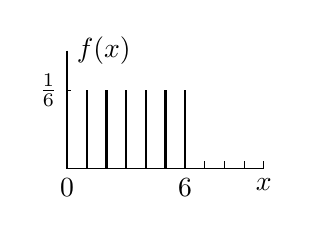
\begin{tikzpicture}[x={0.25cm}]
\draw(0,1.5)node[right]{$f(x)$}--(0,0)--(10,0)node[below]{$x$};
\foreach \x in {7,8,9,10}{\draw(\x,0)--++(0,0.1);}
\draw(0,0)node[below]{$0$} (6,0)node[below]{$6$} (0,1)node[left]{$\frac{1}{6}$}--++(0.2,0);
\foreach \x in {1,2,3,4,5,6}{\draw[thick] (\x,0)--++(0,1);}
\path(0,0)--(-2,0);
\end{tikzpicture}
\begin{tikzpicture}[x={0.25cm}]
\draw(0,3.5)--(0,0)--(10,0)node[below]{$x$};
\foreach \x in {2,3,...,10}{\draw(\x,0)--++(0,0.1);}
\foreach \x/\xx in {1/0,2/1,3/2,4/3,5/4,6/5}{\draw(\x,0.5*\xx)--++(0,0.5)node[circ]{}--++(1,0);}
\draw(7,3)--(10,3);
\foreach \y/\yy in {1.5/0.5,3/1.0}{\draw(0,\y)node[left]{$\yy$}--++(0.2,0);}
\draw(0,3.5)node[right]{$F(x)$};
\path(0,0)--(-2,0);
\end{tikzpicture}
\caption{تفاعل احتمال $f(x)$ اور تفاعل تقسیم $F(x)$}
\label{شکل_شماریات_تفاعل_تقسیم_الف}
\end{minipage}\hfill
\begin{minipage}{0.45\textwidth}
\centering
\begin{tikzpicture}[x={0.25cm}]
\draw(0,1.2)node[right]{$f(x)$}--(0,0)--(15,0)node[below]{$x$};
%\draw(0,0)node[below]{$0$} (6,0)node[below]{$6$} (0,0.5)node[left]{$\frac{1}{6}$}--++(0.2,0);
\foreach \x/\y in {2/1,3/2,4/3,5/4,6/5,7/6,8/5,9/4,10/3,11/2,12/1}{\draw[thick] (\x,0)--++(0,6*\y/36);}
\draw(5,0)node[below]{$5$};
\draw(10,0)node[below]{$10$};
\draw(0,1)node[left]{$\tfrac{1}{6}$}--++(0.2,0);
\path(0,0)--(-2,0);
\end{tikzpicture}
\begin{tikzpicture}[x={0.25cm}]
\draw(0,3.5)--(0,0)--(15,0)node[below]{$x$};
\draw(2,0)\foreach \y in {1,2,3,4,5,6,5,4,3,2,1}{--++(0,3*\y/36)node[circ]{}--++(1,0)};
\draw(13,3)--(15,3);
\draw(0,3.5)node[right]{$F(x)$};
\foreach \x in {1,2,...,15}{\draw(\x,0)--++(0,0.05);}
\draw(5,0)node[below]{$5$} (10,0)node[below]{$10$} ;
\draw(0,3)node[left]{$1$}--++(0.2,0);
\draw (0,5/6)node[left]{$\tfrac{10}{36}$}--++(0.2,0);
\draw (0,5/3)node[left]{$\tfrac{20}{36}$}--++(0.2,0);
\draw (0,5/2)node[left]{$\tfrac{30}{36}$}--++(0.2,0);
\path(0,0)--(-2,0);
\end{tikzpicture}
\caption{تفاعل احتمال $f(x)$ اور تفاعل تقسیم $F(x)$}
\label{شکل_شماریات_تفاعل_تقسیم_ب}
\end{minipage}
\end{figure}
دو پانسہ کے تجربہ میں چونکہ \عددی{6\cdot6=36} ممکنہ مساوی امکانی انجام ہیں لہٰذا ہر ایک کا احتمال \عددی{\tfrac{1}{36}} ہے۔صرف \عددی{(1,1)} کے لئے (جہاں پہلا عدد ایک پانسہ اور دوسرا عدد دوسرے پانسہ کا نتیجہ ہے) \عددی{X=2} ہو گا؛ اسی طرح \عددی{(1,2)} اور \عددی{(2,1)} انجام کے لئے \عددی{X=3} ہو گا؛ \عددی{(1,3)}، \عددی{(2,2)}، \عددی{(3,1)} کے لئے \عددی{X=4} ہو گا، وغیرہ۔

صرف وہ \عددی{x_1,x_2,x_3,\cdots} قیمتیں جن کے لئے بلا منصوبہ غیر مسلسل متغیر \عددی{X} مثبت احتمال رکھتا ہو \عددی{X} کی \اصطلاح{ممکنہ قیمتیں}\فرہنگ{ممکنہ قیمتیں}\حاشیہب{possible values}\فرہنگ{values!possible} کہلاتی ہیں۔جس وقفہ میں کوئی ممکنہ قیمت نہ پائی جاتی اس وقفہ میں تفاعل تقسیم \عددی{F(x)} مستقل ہو گا۔اس طرح \عددی{F(x)} \اصطلاح{سیڑھی تفاعل}\فرہنگ{سیڑھی تفاعل}\فرہنگ{step function} (ٹکڑوں میں مستقل تفاعل) ہو گا جس میں \عددی{x=x_j} پر اوپر رخ \عددی{p_j=P(X=x_j)} چھلانگ پائی جائے گی جبکہ دو چھلانگوں کے بیچ یہ مستقل ہو گا۔شکل \حوالہ{شکل_شماریات_تفاعل_تقسیم_الف} اور شکل \حوالہ{شکل_شماریات_تفاعل_تقسیم_ب} میں ایسا صاف ظاہر ہے۔

ہم اب استمراری بلا منصوبہ متغیر کی تعریف پیش کرتے ہیں اور اس پر غور کرتے ہیں۔ایک بلا منصوبہ متغیر \عددی{X} اور اس کا مطابقتی تفاعل تقسیم تب \اصطلاح{استمراری}\فرہنگ{استمراری}\فرہنگ{continuous} کہلاتے ہیں جب اس کا تفاعل تقسیم \عددی{F(x)=P(X\le x)} مثبت ہو اور اسے درج ذیل تکمل کی صورت میں لکھنا ممکن ہو\حاشیہد{\عددی{F(x)} استمراری ہے لیکن \عددی{F(x)} کے استمراری ہونے سے  مساوات \حوالہ{مساوات_شماریات_استمراری_بلا_منصوبہ_متغیر_الف} کی موجودگی ثابت نہیں ہوتی ہے۔چونکہ ایسے استمراری تفاعل تقسیم جنہیں مساوات \حوالہ{مساوات_شماریات_استمراری_بلا_منصوبہ_متغیر_الف} کی صورت میں لکھنا ممکن نہ ہو عملاً بہت کم پائے جاتے ہیں لہٰذا اصطلاحات "استمراری بلا منصوبہ متغیر" اور "استمراری تقسیم" جو بہت زیادہ استعمال کی جاتی ہیں سے پریشانی پیدا ہونے کا امکان بہت کم ہو گا۔}
\begin{align}\label{مساوات_شماریات_استمراری_بلا_منصوبہ_متغیر_الف}
F(x)=\int_{-\infty}^{x} f(v)\dif v
\end{align}
جہاں متکمل استمراری ہے، ماسوائے  \عددی{v} کی متناہی تعداد  کے قیمتوں کے لئے۔متکمل \عددی{f} کو تقسیم کی \ترچھا{کثافت احتمال} یا مختصراً \اصطلاح{کثافت}\فرہنگ{کثافت}\فرہنگ{density} کہتے ہیں۔ہر اس \عددی{x} پر جہاں \عددی{f(x)} استمراری ہو وہاں مساوات \حوالہ{مساوات_شماریات_استمراری_بلا_منصوبہ_متغیر_الف} کو تقسیم کرتے ہوئے 
\begin{align*}
F'(x)=f(x)
\end{align*}
حاصل ہو گا۔اس لحاظ سے تفاعل تقسیم کا تفرق کثافت ہے۔

مساوات \حوالہ{مساوات_شماریات_استمراری_بلا_منصوبہ_متغیر_الف} اور حصہ \حوالہ{حصہ_شماریات_احتمال} کے مسلمہ-ب کے تحت درج ذیل ہو گا۔
\begin{align}\label{مساوات_شماریات_استمراری_بلا_منصوبہ_متغیر_ب}
\int_{-\infty}^{\infty} f(v)\dif v=1
\end{align}
مساوات \حوالہ{مساوات_شماریات_غیر_مسلسل_متغیر_ث} اور مساوات \حوالہ{مساوات_شماریات_استمراری_بلا_منصوبہ_متغیر_الف} سے درج ذیل کلیہ حاصل ہوتا ہے۔
\begin{align}\label{مساوات_شماریات_استمراری_بلا_منصوبہ_متغیر_پ}
P(a<X\le b)=F(b)-F(a)=\int_{a}^{b}f(v)\dif v
\end{align}
یوں جیسا شکل \حوالہ{شکل_مساوات_شماریات_استمراری_بلا_منصوبہ_متغیر_پ} میں دکھایا گیا ہے، کثافت \عددی{f(x)} کے منحنی کے نیچے \عددی{x=a} اور \عددی{x=b} کے بیچ رقبہ احتمال کے برابر ہو گا۔
\begin{figure}
\centering
\begin{tikzpicture}
\draw(2,2) to [out=0,in=170]coordinate[pos=0.25](kA)coordinate[pos=0.6](kB)(4,0.25);
\draw(2,2) to [out=180,in=10]coordinate[pos=0.25](kN)(0,0.25);
\path(kA)--($(0,0)!(kA)!(4,0)$)coordinate(kD)node[below]{$a$};
\path(kB)--($(0,0)!(kB)!(4,0)$)coordinate(kC)node[below]{$b$};
\shade[gray,shading angle=180] (kA)--(kB)--(kC)--(kD)--(kA);
\draw(kA)--($(0,0)!(kA)!(4,0)$)coordinate(kD)node[below]{$a$};
\draw(kB)--($(0,0)!(kB)!(4,0)$)coordinate(kC)node[below]{$b$};
\draw(0,0)--(4,0)node[below]{$x$};
\draw[stealth-] (kN) to [out=135,in=0]++(-0.5,0.4)node[left]{$f(x)$\,\RL{کثافت}};
\draw[stealth-] ($(kC)!0.5!(kD)$)++(0,1) to [out=45,in=180]++(1,1)node[right]{$P(a<X\le b)$};
\end{tikzpicture}
\caption{شکل برائے مساوات \حوالہ{مساوات_شماریات_استمراری_بلا_منصوبہ_متغیر_پ}}
\label{شکل_مساوات_شماریات_استمراری_بلا_منصوبہ_متغیر_پ}
\end{figure}

ظاہر ہے کہ کسی بھی  مقررہ \عددی{a} اور \عددی{b\,(>a)} کے لئے وقفہ \عددی{a<X\le b}، \عددی{a<X<b} اور \عددی{a\le X<b} کے احتمال ایک جیسے ہوں گے جو غیر مسلسل صورت حال سے مختلف ہے۔

استمراری تقسیم کے مثال (سوالات) اگلے حصے کے سوالات اور آنے والے حصوں میں پیش کئے جائیں گے۔

%=====================
\حصہء{سوالات}
%=============
\ابتدا{سوال}\quad
تفاعل احتمال \عددی{f(x)=\tfrac{x^2}{14}\,\, (x=1,2,3)} اور تفاعل تقسیم کی ترسیم کھینچیں۔
\انتہا{سوال}
%====================
\ابتدا{سوال}\quad
\عددی{X} کا تفاعل احتمال \عددی{f(2)=\tfrac{1}{2}}، \عددی{f(3)=\tfrac{1}{4}}، \عددی{f(4)=f(5)=\tfrac{1}{8}} ہے۔اس کا کیا احتمال ہے کہ \عددی{X} کی قیمت \عددی{4} سے کم ہو گی؟
\انتہا{سوال}
%=====================
\ابتدا{سوال}\quad
ایک مشین کو \عددی{X} سالوں کے بعد تبدیل کرنا ضروری ہے۔\عددی{X} کا تفاعل احتمال \عددی{f(1)=0.3}، \عددی{f(2)=0.4}، \عددی{f(3)=0.2}، \عددی{f(4)=0.1} ہے۔\عددی{f} اور \عددی{F} کو ترسیم کریں۔
\انتہا{سوال}
%====================
\ابتدا{سوال}\quad
کسی پٹرول پمپ میں ایک دن کی درکار پٹرول بلا منصوبہ متغیر \عددی{X} ہے۔ فرض کریں کہ \عددی{2000<x<6000} کے لئے \عددی{X} کی کثافت \عددی{f(x)=k} ہے ورنہ \عددی{0} ہے۔\عددی{k} تلاش کریں اور تفاعل تقسیم \عددی{F(x)} ترسیم کریں۔\\
جواب:\quad
\begin{align*}
k=\tfrac{1}{4000},\quad 
F(x)=
\begin{cases}
0&x<2000\\
\tfrac{x}{4000}-0.5&2000\le x<6000\\
1&x\ge 6000
\end{cases}
\end{align*}
\انتہا{سوال}
%==========================
\ابتدا{سوال}\quad
\عددی{x>0} کے لئے \عددی{f(x)=ce^{-x}} جبکہ \عددی{x<0} کے لئے \عددی{f(x)=0} ہے۔\عددی{c} تلاش کریں۔ \عددی{f} اور \عددی{F} کر ترسیم کریں۔
\انتہا{سوال}
%=======================
\ابتدا{سوال}\quad
\عددی{3} پانسہ اچھال کر ان کا مجموعہ لے کر بلا منصوبہ متغیر \عددی{X} حاصل کیا جاتا ہے۔تفاعل احتمال \عددی{f(x)} ترسیم کریں۔\\
جواب:\quad
$f(3)=\tfrac{1}{216}, f(4)=\tfrac{3}{216},\cdots$
\انتہا{سوال}
%======================
\ابتدا{سوال}\quad
کاغذ کے گتے کی موٹائی \عددی{X} ملی میٹر ہے۔ فرض کریں کہ \عددی{1.9<x<2.1} کے لئے کثافت \عددی{f(x)=kx} ہے ورنہ \عددی{f(x)=0} ہے۔\عددی{k} تلاش کریں۔اس کا کیا احتمال ہے کہ گتے کی موٹائی \عددی{1.95} اور \عددی{2.05} کے بیچ ہو؟
\انتہا{سوال}
%=================
\ابتدا{سوال}\quad
ایک سکہ کو اتنی مرتبہ (\عددی{X})  اچھالا جاتا ہے جب تک خط حاصل نہ ہو۔دکھائیں کہ اس تجربہ کا تفاعل احتمال \عددی{f(x)=2^{-x},\,\, (x=1,2,\cdots)} ہو گا۔دکھائیں کہ \عددی{f(x)} مساوات \حوالہ{مساوات_شماریات_غیر_مسلسل_متغیر_پ} کو مطمئن کرتا ہے۔
\انتہا{سوال}
%=======================
\ابتدا{سوال}\quad
\عددی{0\le x\le 1} کے لئے \عددی{f(x)=kx^2} ہے ورنہ \عددی{f(x)=0} ہے۔\عددی{k} تلاش کریں۔ایسا عدد \عددی{c} تلاش کریں کہ \عددی{P(X\le c)=\SI{72.9}{\percent}} ہو۔
\انتہا{سوال}
%=======================
\ابتدا{سوال}\quad
بلب کی عرصہ زندگی \عددی{X} بلا منصوبہ متغیر ہے جس کی کثافت
\begin{align*}
f(x)=6[0.25-(x-1.5)^2]\quad \quad 1\le x\le 2
\end{align*}
 اور باقی \عددی{x} کے لئے \عددی{f(x)=0} ہے، جہاں \عددی{x=1} سے مراد \عددی{1000} گھنٹے ہیں۔ کیا احتمال ہے کہ سڑک کے اشارے پر پہلے \عددی{1200} گھنٹوں میں تین میں سے کسی ایک بھی بلب کی تبدیل کرنے کی ضرورت پیش نہ آئے؟\\
جواب:\quad
$P(X>1200)=\int_{1.2}^{2}6[0.25-(x-1.5)^2]\dif x=0.896^3=\SI{72}{\percent}$
\انتہا{سوال}
%========================
\ابتدا{سوال}\quad
کسی دکان کی فروخت اور منافع کی نسبت  \عددی{X} ہے۔ فرض کریں کہ \عددی{X} کی تفاعل تقسیم \عددی{x<2} کے لئے \عددی{F(x)=0}، \عددی{2\le x<3} کے لئے \عددی{F(x)=\tfrac{x^2-4}{5}} اور \عددی{x\ge 3} کے لئے \عددی{F(x)=1} ہے۔کثافت تلاش کر کے ترسیم کریں۔\عددی{X} کی  قیمت \عددی{2.5} (\عددی{\SI{40}{\percent}} منافع) اور \عددی{5} (\عددی{\SI{20}{\percent}} منافع) کے بیچ میں ہونے کا کیا احتمال ہے؟  
\انتہا{سوال}
%========================
\ابتدا{سوال}\quad
\عددی{X} ایک بلا منصوبہ متغیر ہے جو کوئی بھی حقیقی قیمت اختیار کر سکتا ہے۔وقوعہ \عددی{X\le b}، \عددی{X<b}، \عددی{X\ge c}، \عددی{X>c}، \عددی{b\le X\le c}، \عددی{b<X\le x} کے متمم کے کیا احتمال ہوں گے؟\\
جواب:\quad
$X\le b \,\text{یا} \,X>c,X<b \,\text{یا} \, X>c,X\le c,X<c,X\ge b,X>b$
\انتہا{سوال}
%=========================
\ابتدا{سوال}\quad
ایک ڈبہ میں \عددی{4} دائیں ہاتھ پیچ اور \عددی{6} بائیں ہاتھ پیچ پائے جاتے ہیں۔بغیر واپس رکھے، دو پیچ بلا منصوبہ نکالے جاتے ہیں۔نکالے گئے بائیں ہاتھ پیچوں کی تعداد \عددی{X} ہے۔ احتمال \عددی{P(X=0)}، \عددی{P(X=1)}، \عددی{P(1<X<2)} \عددی{P(X\le 1)}، \عددی{P(X\ge 1)}، \عددی{P(X>1)}،\عددی{P(0.5<X<10)} تلاش کریں۔
\انتہا{سوال}
%===========================
\ابتدا{سوال}\quad
دکھائیں کہ \عددی{b<c} سے مراد \عددی{P(X\le b)\le P(X\le c)} ہے۔
\انتہا{سوال}
%============================

\حصہ{تقسیم کا اوسط اور  اس کی تغیریت}\شناخت{حصہ_شماریات_تقسیم_کا_اوسط_اور_تغیریت}
\ترچھا{تقسیم} کے \اصطلاح{اوسط}\فرہنگ{اوسط}\حاشیہب{mean}\فرہنگ{mean} کو \عددی{\mu} سے ظاہر کیا جاتا ہے اور اس کی تعریف درج ذیل ہے۔
\begin{gather}
\begin{aligned}\label{مساوات_شماریات_اوسط_تغیریت_الف}
\text{(الف)}\quad\mu&=\sum_{j} x_jf(x_j)\quad\quad \quad (\text{\RL{غیر مسلسل تقسیم}})\\
\text{(ب)}\quad \mu&=\int_{-\infty}^{\infty} xf(x)\dif x\quad\quad\quad (\text{\RL{استمراری تقسیم}})
\end{aligned}
\end{gather}
مساوات \حوالہ{مساوات_شماریات_اوسط_تغیریت_الف}-الف میں زیر غور بلا منصوبہ متغیر \عددی{X} کا تفاعل احتمال \عددی{f(x)} ہے اور ہم تمام ممکنہ قیمتوں (حصہ \حوالہ{حصہ_شماریات_بلا_منصوبہ_متغیرات}) پر مجموعہ لیتے ہیں۔مساوات \حوالہ{مساوات_شماریات_اوسط_تغیریت_الف}-ب میں \عددی{X} کی کثافت \عددی{f(x)} ہے۔اوسط کو \عددی{X} کی \اصطلاح{حسابی توقع}\فرہنگ{حسابی!توقع}\حاشیہب{mathematical expectation}\فرہنگ{expectation!mathematical} بھی کہتے ہیں جس کو \عددی{E(X)} سے ظاہر کیا جاتا ہے۔تعریف کی رو سے ہم فرض کرتے ہیں کہ مساوات \حوالہ{مساوات_شماریات_اوسط_تغیریت_الف}-الف کی تسلسل حتمی مرتکز ہو گی اور \عددی{-\infty} سے \عددی{\infty} تک \عددی{\abs{x}f(x)} کا تکمل موجود ہو گا۔اگر یہ تکمل موجود نہ ہو تب ہم کہتے ہیں کہ اس تقسیم کی اوسط نہیں ہائی جاتی ہے؛ ایسی صورت عملی انجینئری میں شاذ و نادر پائی جاتی ہے۔  

\عددی{x=c} کے لحاظ سے ایک تقسیم کو اس صورت تشاکلی کہتے ہیں جب ہر حقیقی \عددی{x} کے لئے درج ذیل مطمئن ہوتا ہو۔
\begin{align}\label{مساوات_شماریات_اوسط_تغیریت_ب}
f(c+x)=f(c-x)
\end{align} 
آپ درج ذیل مسئلہ ثابت کر سکتے ہیں (سوال \حوالہ{سوال_شماریات_اوسط_الف})۔

%===============
\ابتدا{مسئلہ}\شناخت{مسئلہ_شماریات_تشاکلی_تقسیم_کا_اوسط}\quad \موٹا{(تشاکلی تقسیم کا اوسط)}\\
اگر ایک تقسیم \عددی{x=c} کے لحاظ سے تشاکلی ہو اور اس کا اوسط \عددی{\mu} ہو تب \عددی{\mu=c} ہو گا۔ 
\انتہا{مسئلہ}
%=========================

تقسیم کی \اصطلاح{تغیریت}\فرہنگ{تغیریت}\حاشیہب{variance}\فرہنگ{variance} کو \عددی{\sigma^{\,2}} سے ظاہر کیا جاتا ہے اور اس کی تعریف درج ذیل کلیہ دیتی ہے
\begin{gather}
\begin{aligned}\label{مساوات_شماریات_اوسط_تغیریت_پ}
\text{(الف)}\quad \sigma^{\,2}&=\sum_{j} (x_j-\mu)^2f(x_j)\quad\quad\quad (\text{\RL{غیر مسلسل تقسیم}})\\
\text{(ب)}\quad \sigma^{\,2}&=\int_{-\infty}^{\infty} (x-\mu)^2f(x)\dif x\quad \quad \quad (\text{\RL{استمراری تقسیم}})
\end{aligned}
\end{gather}
جہاں تعریف کی رو سے ہم فرض کرتے ہیں کہ مساوات \حوالہ{مساوات_شماریات_اوسط_تغیریت_پ}-الف میں دی گئی تسلسل حتمی مرتکز ہے اور مساوات \حوالہ{مساوات_شماریات_اوسط_تغیریت_پ}-ب کا تکمل موجود ہے۔

غیر مسلسل تقسیم کی صورت میں اگر کسی ایک نقطہ پر \عددی{f(x)=1} اور باقی ہر جگہ \عددی{f(x)=0} ہو تب \عددی{\sigma^2=0} ہو گا جو عملاً غیر دلچسپ صورت ہے۔اس غیر دلچسپ صورت  کے علاوہ ہر صورت میں درج ذیل ہو گا۔
\begin{align}\label{مساوات_شماریات_اوسط_تغیریت_ت}
\sigma^{\,2}>0
\end{align}

تغیریت کا مثبت جذر \اصطلاح{معیاری انحراف}\فرہنگ{معیاری انحراف}\فرہنگ{انحراف!معیاری}\حاشیہب{standard deviation}\فرہنگ{standard deviation} کہلاتا ہے جس کو \عددی{\sigma} سے ظاہر کیا جاتا ہے۔ 

بلا منصوبہ متغیر \عددی{X} جن قیمتوں کو اختیار کر سکتا ہے، تغیریت کو ان قیمتوں کی پھیل کی ناپ تصور کیا جا سکتا ہے۔ 

%=================
\ابتدا{مثال}\quad \موٹا{(اوسط اور تغیریت)}\\
بلا منصوبہ متغیر
\begin{align*}
X=\text{\RL{سکہ اچھال کر شیر کا حاصل ہونا}}
\end{align*}
کے ممکنہ قیمتیں \عددی{X=0} اور \عددی{X=1} ہیں جن کا احتمال \عددی{P(X=0)=\tfrac{1}{2}} اور \عددی{P(X=1)=\tfrac{1}{2}} ہے۔مساوات \حوالہ{مساوات_شماریات_اوسط_تغیریت_الف}-الف سے اوسط \عددی{\mu=0\cdot \tfrac{1}{2}+1\cdot\tfrac{1}{2}=\tfrac{1}{2}} حاصل ہوتا ہے۔مساوات \حوالہ{مساوات_شماریات_اوسط_تغیریت_الف}-ب سے درج ذیل حاصل ہو گا۔
\begin{align*}
\sigma^{\,2}=(0-\tfrac{1}{2})^2\cdot \tfrac{1}{2}+(1-\tfrac{1}{2})^2\cdot \tfrac{1}{2}=\tfrac{1}{4}
\end{align*}
\انتہا{مثال}
%=======================
\ابتدا{مثال}\quad \موٹا{یکساں تقسیم}\\
وہ تقسیم جس کی کثافت \عددی{a<x<b} کے لئے
\begin{align*}
f(x)=\frac{1}{b-a}\quad \quad (a<x<b\,\,\text{جب})
\end{align*}
اور باقی \عددی{x} کے لئے \عددی{f=0} ہو، وقفہ \عددی{a<x<b} میں \اصطلاح{یکساں تقسیم}\فرہنگ{تقسیم!یکساں}\حاشیہب{uniform distribution}\فرہنگ{distribution!uniform} کہلاتی ہے۔ مسئلہ \حوالہ{مسئلہ_شماریات_تشاکلی_تقسیم_کا_اوسط} یا مساوات \حوالہ{مساوات_شماریات_اوسط_تغیریت_پ}-الف سے \عددی{\mu=\tfrac{a+b}{2}} اور مساوات \حوالہ{مساوات_شماریات_اوسط_تغیریت_پ}-ب سے  تغیریت حاصل کرتے ہیں۔
\begin{align*}
\sigma^{\,2}=\int_a^b (x-\tfrac{a+b}{2})^2\tfrac{1}{b-a}\dif x=\frac{(b-a)^2}{12}
\end{align*}
شکل \حوالہ{شکل_شماریات_یکساں_تقسیم_اوسط_تغیریت} میں چند خصوصی مثالیں پیش کی گئی ہیں جو دکھاتی ہیں کہ \عددی{\sigma^{\,2}} پھیل کی ناپ ہے۔ 
\انتہا{مثال}
%===========================
\begin{figure}
\centering
\begin{subfigure}{0.5\textwidth}
\centering
\begin{tikzpicture}
\draw(-0.5,0)--(1.5,0)node[right]{$x$};
\draw(0,0)--(0,1.5)node[right]{$f(x)$};
\draw[thick] (-0.5,0)--(0,0)node[below]{$0$}--(0,1)node[left]{$1$}--(1,1)--(1,0)node[below]{$1$}--(1.5,0);
\draw(1,1)node[above right]{$(\sigma^{\,2}=\tfrac{1}{12})$};
\path(3,0)--(3.5,0);
\end{tikzpicture}
\end{subfigure}%
\begin{subfigure}{0.5\textwidth}
\centering
\begin{tikzpicture}
\draw(-1.5,0)--(2.5,0)node[right]{$x$};
\draw(0,0)node[below]{$0$}--(0,1.5)node[right]{$f(x)$};
\draw[thick](-1.5,0)--(-1,0)node[below]{$-1$}--(-1,1/3)--(2,1/3)--(2,0)node[below]{$2$}--(2.5,0);
\draw(0,1)node[left]{$1$}--++(0.2,0);
\draw(1,1)node[above right]{$(\sigma^{\,2}=\tfrac{3}{4})$};
\end{tikzpicture}
\end{subfigure}
\begin{subfigure}{0.5\textwidth}
\centering
\begin{tikzpicture}
\draw(0,0)--(0,1.5)node[right]{$F(x)$};
\draw(-0.5,0)--(1.5,0)node[right]{$x$};
\draw[thick](-0.5,0)--(0,0)--(1,1)--(1.5,1);
\draw(1,0)node[below]{$1$}--++(0,0.2);
\draw(0,1)node[left]{$1$}--++(0.2,0);
\path(3,0)--(3.5,0);
\end{tikzpicture}
\end{subfigure}%
\begin{subfigure}{0.5\textwidth}
\centering
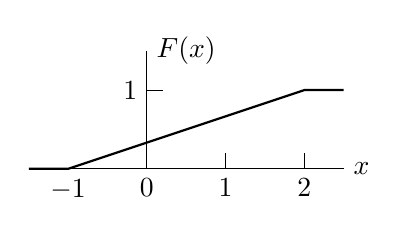
\begin{tikzpicture}
\draw(-1.5,0)--(2.5,0)node[right]{$x$};
\draw(0,0)node[below]{$0$}--(0,1.5)node[right]{$F(x)$};
\draw[thick](-1.5,0)--(-1,0)node[below]{$-1$}--(2,1)--(2.5,1);
\draw(1,0)node[below]{$1$}--++(0,0.2);
\draw(2,0)node[below]{$2$}--++(0,0.2);
\draw(0,1)node[left]{$1$}--++(0.2,0);
\end{tikzpicture}
\end{subfigure}%
\caption{یکساں تقسیم جن کی ایک جیسی اوسط \عددی{(0.5)} لیکن مختلف تغیریت \عددی{\sigma^{\,2}} ہے}
\label{شکل_شماریات_یکساں_تقسیم_اوسط_تغیریت}
\end{figure}

%==================
\ابتدا{مسئلہ}\شناخت{مسئلہ_شماریات_خطی_تبادل}\quad \موٹا{(خطی تبادل)}\\
اگر بلا منصوبہ متغیر \عددی{X} کی اوسط \عددی{\mu} اور تغیریت \عددی{\sigma^{\,2}} ہو تب بلا منصوبہ متغیر \عددی{X^*=c_1X+c_2\,(c_1\ne 0)} کی اوسط
\begin{align}\label{مساوات_شماریات_اوسط_تغیریت_ٹ}
\mu^*=c_1\mu+c_2
\end{align}
 اور تغیریت
\begin{align}\label{مساوات_شماریات_اوسط_تغیریت_ث}
\sigma^{*2}=c_1^{\,2}\sigma^{\,2}
\end{align}
ہو گی۔
\انتہا{مسئلہ}
%=======================
\ابتدا{ثبوت}\quad
ہم پہلے \عددی{c_1>0} فرض کرتے ہوئے مساوات \حوالہ{مساوات_شماریات_اوسط_تغیریت_ٹ} کو استمراری صورت کے لئے ثابت کرتے ہیں۔چونکہ \عددی{X} محور پر چھوٹے سے وقفہ \عددی{\Delta x} کا مطابقتی احتمال (تخمیناً) \عددی{f(x)\Delta x} ہو گا جو ہر صورت \عددی{X^*} محور پر مطابقتی چھوٹے وقفہ \عددی{\Delta x^*=c_1\Delta x} پر احتمال \عددی{f^*(x^*)\Delta x^*} کے برابر ہو گا لہٰذا \عددی{x} اور \عددی{x^*=c_1x+c_2} کے مطابقتی، \عددی{X} کی کثافت \عددی{f(x)} اور \عددی{X^*} کی کثافت \عددی{f^*(x^*)}،  تعلق \عددی{f^*(x^*)=\tfrac{f(x)}{c_1}} کو مطمئن کریں گے۔چونکہ \عددی{\tfrac{\dif x^*}{\dif x}=c_1} ہے لہٰذا \عددی{\dif x^*=c_1\dif x} اور \عددی{f^*(x^*)\dif x^*=f(x)\dif x} ہو گا۔یوں درج ذیل ہو گا
\begin{align*}
\mu^*=\int_{-\infty}^{\infty} x^*f^*(x^*)\dif x^*&=\int_{-\infty}^{\infty} (c_1x+c_2)f(x)\dif x\\
&=c_1\int_{-\infty}^{\infty}xf(x)\dif x+c_2\int_{-\infty}^{\infty}f(x)\dif x
\end{align*}
جہاں آخری تکمل مساوات \حوالہ{مساوات_شماریات_استمراری_بلا_منصوبہ_متغیر_ب} کے تحت \عددی{1} کے برابر ہو گا۔یوں  مساوات \حوالہ{مساوات_شماریات_اوسط_تغیریت_ٹ} ثابت ہوتی ہے۔چونکہ
\begin{align*}
x^*-\mu^*=(c_1x+c_2)-(c_1\mu+c_2)=c_1x-c_1\mu
\end{align*}
ہے لہٰذا تغیریت کی تعریف سے
\begin{align*}
\sigma^{*2}=\int_{-\infty}^{\infty} (x^*-\mu^*)^2f^*(x^*)\dif x^*=\int_{-\infty}^{\infty} (c_1x-c_1\mu)^2f(x)\dif x=c_1^2\sigma^2
\end{align*}
حاصل ہو گا۔ \عددی{c_1<0} سے نتائج تبدیل نہیں ہوتے ہیں چونکہ اس سے دو اضافی منفی کی علامتیں ملتی ہیں، ایک \عددی{x} میں تکمل کے رخ کی تبدیلی کی بنا (دھیان رہے کہ \عددی{x^*=-\infty} کا مطابقتی \عددی{x=\infty} ہے) اور دوسرا \عددی{f^*(x^*)=\tfrac{f(x)}{-c_1}} کی بنا؛ یہاں \عددی{-c_1>0} درکار ہو گا چونکہ کثافت غیر منفی قیمت ہے۔  

غیر مسلسل کثافت کے لئے مسئلے کا ثبوت بھی بالکل ایسا ہی ہے۔ 
\انتہا{ثبوت}
%========================

مساوات \حوالہ{مساوات_شماریات_اوسط_تغیریت_ٹ} اور مساوات \حوالہ{مساوات_شماریات_اوسط_تغیریت_ث} سے ہم درج ذیل اخذ کر سکتے ہیں۔

%=========================
\ابتدا{مسئلہ}\شناخت{مسئلہ_شماریات_معیاری_متغیر}\quad \موٹا{(معیاری متغیر)}\\
اگر بلا منصوبہ متغیر \عددی{X} کی اوسط \عددی{\mu} اور تغیریت \عددی{\sigma^2} ہو، تب مطابقتی متغیر \عددی{Z=\tfrac{X-\mu}{\sigma}} کی اوسط \عددی{0} اور تغیریت \عددی{1} ہو گی۔
\انتہا{مسئلہ}
%==============================

\عددی{Z} کو \عددی{X} کا مطابقتی \اصطلاح{معیاری متغیر}\فرہنگ{معیاری!متغیر}\حاشیہب{standardized variable}\فرہنگ{variable!standardized} کہتے ہیں۔

اگر \عددی{X} کوئی بلا منصوبہ متغیر اور \عددی{g(X)} کوئی استمراری تفاعل ہو جو تمام حقیقی \عددی{X} کے لئے معین ہو تب عدد
\begin{gather}
\begin{aligned}\label{مساوات_شماریات_اوسط_تغیریت_ج}
\text{(الف)}\quad E(g(X))&=\sum_j g(x_j)f(x_j)\quad\quad (X\,\text{\RL{غیر مسلسل}})\\
\text{(ب)}\quad E(g(X))&=\int_{-\infty}^{\infty} g(x)f(x)\dif x\quad\quad (X\,\text{\RL{استمرای}}) 
\end{aligned}
\end{gather}
کو \عددی{g(X)} کی \اصطلاح{حسابی توقع}\فرہنگ{توقع!حسابی}\حاشیہب{mathematical expectation}\فرہنگ{expectation!mathematical} کہتے ہیں۔ یہاں \عددی{f} بالترتیب تفاعل احتمال یا کثافت ہے۔

مساوات \حوالہ{مساوات_شماریات_اوسط_تغیریت_ج} میں \عددی{g(X)=X^k\,\, (k=1,2,\cdots)} لیتے ہوئے بالترتیب 
\begin{align}
E(X^k)=\int_{-\infty}^{\infty} x^kf(x)\dif x\quad \text{اور}\quad E(X^k)=\sum_j x_j^k f(x_j)
\end{align}
حاصل ہوتے ہیں۔ \عددی{E(X^k)} کو \عددی{X} کا \اصطلاح{\عددی{k} واں معیار اثر}\فرہنگ{معیار اثر}\حاشیہب{kth moment}\فرہنگ{moment!k} کہتے ہیں۔مساوات \حوالہ{مساوات_شماریات_اوسط_تغیریت_ج} میں \عددی{g(X)=(X-\mu)^k} لیتے ہوئے بالترتیب
\begin{align}
E([X-\mu]^k)=\int_{-\infty}^{\infty} (x-\mu)^kf(x)\dif x\quad \text{اور}\quad E([X-\mu]^k)=\sum_j(x_j-\mu)^kf(x_j)
\end{align}
حاصل ہوتے ہیں  جنہیں \عددی{X} کے \اصطلاح{\عددی{k} ویں وسطی معیار اثر}\فرہنگ{معیار اثر!وسطی}\حاشیہب{kth central moment}\فرہنگ{moment!central, kth} کہتے ہیں۔آپ درج ذیل ثابت کر سکتے ہیں۔
\begin{align}
E(1)&=1\label{مساوات_شماریات_وسطی_معیار_اثر_الف}\\
\mu&=E(X)\label{مساوات_شماریات_وسطی_معیار_اثر_ب}\\
\sigma^2&=E([X-\mu]^2)\label{مساوات_شماریات_وسطی_معیار_اثر_پ}
\end{align}

%=================
\حصہء{سوالات}

%======================
\ابتدا{سوال}\شناخت{سوال_شماریات_اوسط_الف}\quad
مسئلہ \حوالہ{مسئلہ_شماریات_تشاکلی_تقسیم_کا_اوسط} ثابت کریں۔\\
جواب:\quad
\begin{align*}
&\mu=\int_{-\infty}^{c} tf(t)\dif t+\int_{c}^{\infty}tf(t)\dif t\\
&=-\int_{\infty}^{0}(c-x)f(c-x)\dif x+\int_{0}^{\infty}(c+x)f(c+x)\dif x=2c\int_{0}^{\infty}f(c+x)\dif x=c
\end{align*}
غیر مسلسل تقسیم کے لئے بھی ثبوت اسی طرح حاصل کیا جا سکتا ہے۔
\انتہا{سوال}
%===================
\ابتدا{سوال}\quad
ایک تقسیم کی کثافت  \عددی{f(x)=\tfrac{1}{2}e^{-\abs{x}}} ہے۔اس  کی اوسط اور تغیریت تلاش کریں۔\\
جواب:\quad
$\mu=0,\sigma^2=2$
\انتہا{سوال}
%======================
\ابتدا{سوال}\شناخت{سوال_شماریات_اوسط_پ}\quad
\عددی{0\le x\le 2} کے لئے \عددی{X} کی کثافت \عددی{f(x)=0.5x} ہے جبکہ باقی \عددی{x} کے لئے \عددی{f(x)=0} ہے۔دکھائیں کہ \عددی{X} کی اوسط \عددی{\tfrac{4}{3}} اور تغیریت \عددی{\tfrac{2}{9}} ہے۔
\انتہا{سوال}
%==========================
\ابتدا{سوال}\quad
\عددی{Y=-2X+5} کی اوسط اور تغیریت تلاش کریں۔ بلا منصوبہ متغیر \عددی{X} سوال \حوالہ{سوال_شماریات_اوسط_پ} میں دیا گیا ہے۔
\انتہا{سوال}
%============================
\ابتدا{سوال}\quad
سوال \حوالہ{سوال_شماریات_اوسط_پ} کے \عددی{X} کا مطابقتی معیاری بلا منصوبہ متغیر  تلاش کریں۔\\
جواب:\quad
$\tfrac{X-\tfrac{4}{3}}{\sqrt{\tfrac{2}{9}}}$
\انتہا{سوال}
%===========================
\ابتدا{سوال}\quad
مسئلہ \حوالہ{مسئلہ_شماریات_خطی_تبادل} کو غیر مسلسل صورت کے لئے ثابت کریں۔
\انتہا{سوال}
%============================
\ابتدا{سوال}\quad
مسئلہ \حوالہ{مسئلہ_شماریات_معیاری_متغیر} کو مساوات \حوالہ{مساوات_شماریات_اوسط_تغیریت_ٹ} اور مساوات \حوالہ{مساوات_شماریات_اوسط_تغیریت_ث} سے اخذ کریں۔\\
جواب:\quad مساوات \حوالہ{مساوات_شماریات_اوسط_تغیریت_ٹ} اور مساوات \حوالہ{مساوات_شماریات_اوسط_تغیریت_ث} میں \عددی{c_1=\tfrac{1}{\sigma}} اور \عددی{c_2=-\tfrac{\mu}{\sigma}} پر کریں۔
\انتہا{سوال}
%=========================
\ابتدا{سوال}\quad
ایک مخصوص قسم کے ٹائر بلا منصوبہ متغیر \عددی{X} (ہزار کلو میٹر) چلتے ہیں۔\عددی{X} کی کثافت \عددی{x>0} کے لئے \عددی{f(x)=\theta e^{-\theta x}} ورنہ \عددی{0} ہے جہاں \عددی{\theta\,(>0)} مقدار معلوم ہے۔ (الف) ایسے ایک ٹائر سے کتنے کلومیٹر طے کیے جا سکتے ہیں؟ (ب) اگر \عددی{\theta=0.05} ہو تب کم سے کم \عددی{\num{30000}} کلومیٹر تک پہنچنے کا احتمال کیا ہو گا؟
\انتہا{سوال}
%==========================
\ابتدا{سوال}\شناخت{سوال_شماریات_کیل_پیداوار_الف}\quad
ایک کارخانے میں کیل بنائے جاتے ہیں جن کا وتر \عددی{X} سنٹی میٹر ہے۔فرض کریں کہ \عددی{X} کی کثافت \عددی{0.9<x<1.1} کے لئے \عددی{f(x)=k(x-0.9)(1.1-x)} ورنہ \عددی{0} ہے۔\عددی{k} معلوم کریں، \عددی{f(x)} کو ترسیم کریں اور \عددی{\mu} اور \عددی{\sigma^2} کو تلاش کریں۔ \\
جواب:\quad
$k=750,\mu=1,\sigma^2=0.002$
\انتہا{سوال}
%========================
\ابتدا{سوال}\quad
سوال \حوالہ{سوال_شماریات_کیل_پیداوار_الف} میں اگر کیل کے وتر کا \عددی{\SI{1}{\centi\meter}} سے انحراف \عددی{\SI{0.06}{\centi\meter}} بڑھ جائے تب اس کو عیب دار تصور کیا جاتا ہے۔کتنے فی صد کیل عیب دار ہوں گے؟
\انتہا{سوال}
%=============================
\ابتدا{سوال}\شناخت{سوال_شماریات_پٹرول_پمپ_الف}\quad
ایک پٹرول پمپ کو ہر جمعرات دوپہر کے وقت  پٹرول مہیا کیا جاتا ہے۔فروخت پٹرول کا حجم \عددی{X} ہزار لٹر ہے۔ \عددی{0\le x\le 1} کے لئے \عددی{X} کی کثافت احتمال \عددی{f(x)=6x(1-x)} ورنہ \عددی{0} ہے۔ اوسط اور تغیریت تلاش کریں۔\\
جواب:\quad
$\mu=\tfrac{1}{2},\,\sigma^2=\tfrac{1}{20}$
\انتہا{سوال}
%==============================
\ابتدا{سوال}\quad
سوال \حوالہ{سوال_شماریات_پٹرول_پمپ_الف}  میں پٹرول کی ٹینکی کا حجم کتنا ہو گا اگر ایک ہفتہ میں ٹینکی خالی ہونے کا احتمال \عددی{\SI{10}{\percent}} ہو؟
\انتہا{سوال}
%===========================
\ابتدا{سوال}\quad
مساوات \حوالہ{مساوات_شماریات_وسطی_معیار_اثر_الف}، مساوات \حوالہ{مساوات_شماریات_وسطی_معیار_اثر_ب} اور مساوات \حوالہ{مساوات_شماریات_وسطی_معیار_اثر_پ} ثابت کریں۔
\انتہا{سوال}
%===========================
\ابتدا{سوال}\شناخت{سوال_شماریات_تغیریت_دوسرا_کلیہ}\quad
دکھائیں کہ \عددی{E(X-\mu)=0} اور \عددی{\sigma^{\,2}=E(X^2)-\mu^2} ہوں گے۔
\انتہا{سوال}
%============================
\ابتدا{سوال}\quad
فرض کریں کہ \عددی{X} کی کثافت \عددی{0<x<1} کے لئے \عددی{f(x)=2x} ورنہ \عددی{0} ہے۔ تمام معیار اثر تلاش کریں۔سوال \حوالہ{سوال_شماریات_تغیریت_دوسرا_کلیہ} میں دیے گئے کلیہ سے \عددی{\sigma^{\,2}} حاصل کریں۔\\
جواب:\quad
$E(X^k)=\tfrac{2}{k+2},\,\,\sigma^{\,2}=\tfrac{1}{18}$
\انتہا{سوال}
%============================
\ابتدا{سوال}\شناخت{سوال_شماریات_خطی_مجموعہ_کلیہ}\quad
دکھائیں کہ \عددی{E(ag(X)+bh(X))=aE(g(X))+bE(h(X))} ہو گا جہاں \عددی{a} اور \عددی{b} مستقل ہیں۔
\انتہا{سوال}
%========================
\ابتدا{سوال}\quad
وقفہ \عددی{0\le x\le 1} پر یکساں تقسیم کے معیار اثر تلاش کریں۔\\
جواب:\quad
$E(X^k)=\tfrac{1}{k+1}$
\انتہا{سوال}
%==========================
\ابتدا{سوال}\quad \موٹا{(ترچھاپن)} \quad
عدد \عددی{\gamma=\tfrac{1}{\sigma^3}E([X-\mu]^3)} کو \عددی{X} کا \اصطلاح{ترچھاپن}\فرہنگ{ترچھاپن}\حاشیہب{skewness}\فرہنگ{skewness} کہتے ہیں۔اس اصطلاح کا جواز پیش کرنے کی خاطر دکھائیں کہ \عددی{\mu} کے لحاظ سے تشاکلی \عددی{X} کے لئے اگر تیسرا وسطی معیار اثر موجود ہو تب یہ معیار اثر صفر ہو گا۔ 
\انتہا{سوال}
%==============================
\ابتدا{سوال}\quad
\عددی{x>0} کے لئے کثافت تقسیم  \عددی{f(x)=xe^{-x}} ورنہ \عددی{f=0} کی صورت میں کثافت تقسیم کا ترچھاپن تلاش کریں۔\عددی{f(x)} کو ترسیم کریں۔\\
جواب:\quad 
تکمل بالحصص لیں\quad
$\sigma^{\,2}=2,\gamma=\tfrac{4}{2\sqrt{2}}=\sqrt{2}$
\انتہا{سوال}
%========================================
\ابتدا{سوال}\شناخت{سوال_شماریات_معیار_اثر_پیدا_کار_تفاعل_الف}\quad \موٹا{(معیار اثر کا پیدا کار تفاعل)}\\
بلا منصوبہ غیر مسلسل یا استمراری متغیر \عددی{X} کے معیار اثر کا پیدا کار تفاعل درج ذیل کلیات دیتے ہیں
\begin{align*}
G(t)=E(e^{tX})=\sum_j e^{tx_j}f(x_j)\quad \text{اور}\quad G(t)=E(e^{tX})=\int_{-\infty}^{\infty} e^{tx}f(x)\dif x
\end{align*} 
جہاں فرض کیا گیا ہے کہ مجموعہ کی علامت کے اندر اور تکمل کی علامت کے اندر تفرق لیا جا سکتا ہے۔دکھائیں کہ \عددی{E(X^k)=G^{(k)}(0)} ہو گا اور بالخصوص \عددی{\mu=G'(0)} ہو گا جہاں \عددی{G^{(k)}(t)} سے مراد \عددی{t} کے لحاظ سے \عددی{G} کا \عددی{k} واں تفرق ہے۔
\انتہا{سوال}
%==============================

\حصہ{ثنائی، پوئسن، اور بیش ہندسی تقسیم}
ہم اب چند مخصوص غیر مسلسل تقسیم پر غور کرتے ہیں جو شماریات کے لئے اہم ہیں۔

\جزوحصہء{ثنائی تقسیم}
ہم ایک تجربہ کو \عددی{n} مرتبہ بلا منصوبہ سرانجام دینے میں وقوعہ \عددی{A} کے واقع ہونے  کی تعداد سے حاصل ثنائی تقسیم پر غور کرتے ہیں جہاں ایک کوشش میں \عددی{A} کا احتمال \عددی{P(A)=p} فرض کیا جائے گا۔تب ایک کوشش میں \عددی{A} کے نا واقع ہونے کا احتمال \عددی{q=1-p} ہو گا۔یہ تجربہ \عددی{n} مرتبہ سرانجام دیتے ہوئے ہم بلا منصوبہ متغیر
\begin{align*}
X=\text{\RL{واقع ہونے کی تعداد}}\,A
\end{align*}
پر غور کرتے ہیں۔تب \عددی{X} کی قیمتیں \عددی{0,1,\cdots,n} ہو سکتی ہیں۔ہمیں ان اعداد کے مطابقتی احتمال تلاش کرنا چاہتے ہیں۔اس مقصد کے لئے ہم ان قیمتوں میں سے کوئی ایک قیمت، مثلاً \عددی{X=x} پر غور کرتے ہیں جس کا مطلب ہے کہ \عددی{n} میں سے \عددی{x} کوششوں میں \عددی{A} واقع ہوا ہے جبکہ \عددی{n-x} کوششوں میں \عددی{A} واقع نہیں ہوا ہے۔یہ سب کچھ یوں
\begin{align}\label{مساوات_شماریات_ثنائی_تقسیم_الف}
\underbrace{AA\cdots A}_{\text{مرتبہ}\,x}\underbrace{BB\cdots B}_{\text{مرتبہ}\,n-x}
\end{align}
نظر آئے گا۔یہاں \عددی{B=A^C} ہے؛ یعنی \عددی{A} واقع نہیں ہوا ہے۔ہم فرض کرتے ہیں کہ تمام کوششیں بلا منصوبہ ہے یعنی  یہ ایک دوسرے پر اثر انداز نہیں ہوتی ہیں۔تب چونکہ \عددی{ُP(A)=p} اور \عددی{ُP(B)=q}  ہیں لہٰذا مساوات \حوالہ{مساوات_شماریات_ثنائی_تقسیم_الف} کا مطابقتی احتمال 
\begin{align*}
\underbrace{pp\cdots p}_{\text{مرتبہ}\,x}\underbrace{qq\cdots q}_{\text{مرتبہ}\,n-x}=p^xq^{n-x}
\end{align*}
ہو گا۔ظاہر ہے کہ \عددی{x} گنا \عددی{A} اور \عددی{n-x} گنا \عددی{B} کو مختلف انداز (ترتیب) میں لکھنے  کا ایک طریقہ  مساوات \حوالہ{مساوات_شماریات_ثنائی_تقسیم_الف} دیتا ہے لہٰذا  مسئلہ \حوالہ{مسئلہ_شماریات_قاعدہ_جمع_بلا_شرکت_وقوعات} کے تحت \عددی{p^xq^{n-x}} کو  \عددی{x} گنا \عددی{A} اور \عددی{n-x} گنا \عددی{B} کے کل مختلف انداز میں لکھنے کی تعداد سے ضرب دینے سے احتمال \عددی{P(X=x)} حاصل ہو گا۔ہم \عددی{n} کوششوں کو \عددی{1} تا \عددی{n} سے ظاہر کرتے ہوئے ان میں سے ان \عددی{x} کوششوں منتخب کرتے ہیں جن میں \عددی{A} واقع پذیر ہوا ہو۔چونکہ \عددی{x} منتخب کرنے کی ترتیب اہمیت نہیں رکھتی ہے لہٰذا مساوات \حوالہ{مساوات_شماریات_مرتب_اجتماعات_ب} کے تحت \عددی{n} میں سے \عددی{x} کا انتخاب \عددی{\binom{n}{x}} مختلف انداز سے کیا جا سکتا ہے۔یوں \عددی{X=x} کا مطابقتی احتمال \عددی{P(X=x)} 
\begin{align}\label{مساوات_شماریات_ثنائی_تقسیم_ب}
f(x)=\binom{n}{x}p^xq^{n-x}\quad\quad\quad (x=0,1,\cdots,n)
\end{align}
ہو گا جبکہ \عددی{x} کے کسی دوسری قیمت کے لئے \عددی{f(x)=0} ہو گا۔\عددی{n} کوششوں میں ٹھیک \عددی{x} مرتبہ \عددی{A} واقع ہونا کا احتمال  مساوات \حوالہ{مساوات_شماریات_ثنائی_تقسیم_ب} دیتی ہے جہاں ایک کوشش میں \عددی{A} واقع ہونے کا احتمال \عددی{p} ہے اور \عددی{q=1-p} ہے۔مساوات \حوالہ{مساوات_شماریات_ثنائی_تقسیم_ب} میں دی گئی تقسیم کو \اصطلاح{ثنائی تقسیم}\فرہنگ{ثنائی!تقسیم}\فرہنگ{تقسیم!ثنائی}\حاشیہب{binomial distribution}\فرہنگ{binomial!distribution} کہتے ہیں۔\عددی{A} کے واقع ہونے کو \ترچھا{کامیابی}\فرہنگ{کامیابی}\حاشیہب{success}\فرہنگ{success} جبکہ اس کے نا واقع ہونے کو \ترچھا{ناکامی}\فرہنگ{ناکامی}\حاشیہب{failure}\فرہنگ{failure} کہتے ہیں۔ \عددی{p} کو ایک کوشش میں کامیابی  کا احتمال کہتے ہیں۔شکل \حوالہ{شکل_شماریات_ثنائی_مثالیں} میں \عددی{n=5} اور مختلف \عددی{p} کے لئے مساوات \حوالہ{مساوات_شماریات_ثنائی_تقسیم_ب} ترسیم کیا گیا ہے۔
\begin{figure}
\centering
\begin{subfigure}{0.2\textwidth}
\centering
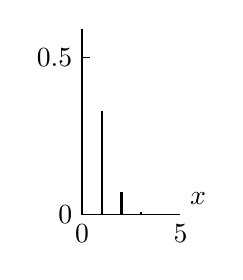
\begin{tikzpicture}[x={0.25cm},y={4cm}]
\foreach \x/\y in {0/0.59,1/0.328,2/0.0723,3/0.0081}{\draw[thick](\x,0)--++(0,\y);}
\draw(0,0)node[left]{$0$}node[below]{$0$}--(5,0)node[below]{$5$}node[above right]{$x$};
\draw(0,0.5)node[left]{$0.5$}--++(0.4,0);
\end{tikzpicture}
\caption*{$p=0.1$}
\end{subfigure}%
\begin{subfigure}{0.2\textwidth}
\centering
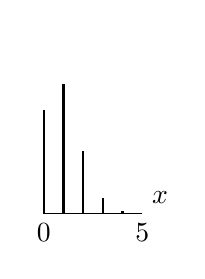
\begin{tikzpicture}[x={0.25cm},y={4cm}]
\foreach \x/\y in {0/0.328,1/0.41,2/0.2,3/0.05,4/0.0064}{\draw[thick](\x,0)--++(0,\y);}
\draw(0,0)node[below]{$0$}--(5,0)node[below]{$5$}node[above right]{$x$};
\path(0,0)--++(0,0.59);
\end{tikzpicture}
\caption*{$p=0.2$}
\end{subfigure}%
\begin{subfigure}{0.2\textwidth}
\centering
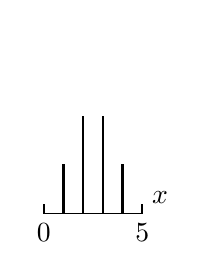
\begin{tikzpicture}[x={0.25cm},y={4cm}]
\foreach \x/\y in {0/0.031,1/0.156,2/0.31,3/0.31,4/0.156,5/0.031}{\draw[thick](\x,0)--++(0,\y);}
\draw(0,0)node[below]{$0$}--(5,0)node[below]{$5$}node[above right]{$x$};
\path(0,0)--++(0,0.59);
\end{tikzpicture}
\caption*{$p=0.5$}
\end{subfigure}%
\begin{subfigure}{0.2\textwidth}
\centering
\begin{tikzpicture}[x={0.25cm},y={4cm}]
\foreach \x/\y in {0/0,1/0.006,2/0.051,3/0.2,4/0.41,5/0.033}{\draw[thick](\x,0)--++(0,\y);}
\draw(0,0)node[below]{$0$}--(5,0)node[below]{$5$}node[above right]{$x$};
\path(0,0)--++(0,0.59);
\end{tikzpicture}
\caption*{$p=0.8$}
\end{subfigure}%
\begin{subfigure}{0.2\textwidth}
\centering
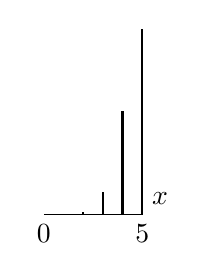
\begin{tikzpicture}[x={0.25cm},y={4cm}]
\foreach \x/\y in {0/0,1/0,2/0.008,3/0.073,4/0.33,5/0.59}{\draw[thick](\x,0)--++(0,\y);}
\draw(0,0)node[below]{$0$}--(5,0)node[below]{$5$}node[above right]{$x$};
\end{tikzpicture}
\caption*{$p=0.9$}
\end{subfigure}%
\caption{مختلف \عددی{p} اور \عددی{n=5} کے لئے مساوات \حوالہ{مساوات_شماریات_ثنائی_تقسیم_ب} میں دی گئی تثنائی تقسیم}
\label{شکل_شماریات_ثنائی_مثالیں}
\end{figure}

ثنائی تقسیم کی اوسط (سوال \حوالہ{سوال_شماریات_ثنائی_ثبوت_الف})
\begin{align}\label{مساوات_شماریات_ثنائی_تقسیم_پ}
\mu=np
\end{align}
اور تغیریت  (سوال \حوالہ{سوال_شماریات_ثنائی_ثبوت_الف})
\begin{align}\label{مساوات_شماریات_ثنائی_تقسیم_ت}
\sigma^{\,2}=npq
\end{align}
ہے۔دھیان رہے کہ \عددی{p=0.5} پر \عددی{\mu} کے لحاظ سے تقسیم تشاکلی ہے۔

\جزوحصہء{پوئسن تقسیم}
ایسی غیر مسلسل تقسیم جس کا تفاعل احتمال درج ذیل ہو \اصطلاح{پوئسن تقسیم}\فرہنگ{پوئسن!تقسیم}\فرہنگ{تقسیم!پوئسن}\حاشیہب{Poisson distribution}\فرہنگ{distribution!Poisson} کہلاتی\حاشیہد{سمیوں دنی پوسوں} ہے۔ 
\begin{align}\label{مساوات_شماریات_پوئسن_تقسیم_الف}
f(x)=\frac{\mu^x}{x!}e^{-\mu}
\end{align}
شکل \حوالہ{شکل_شماریات_پوئسن_مثالیں} میں \عددی{n=5} اور مختلف \عددی{\mu} کے لئے  مساوات \حوالہ{مساوات_شماریات_پوئسن_تقسیم_الف} میں دی گئی پوئسن تقسیم ترسیم کی گئی ہے۔\عددی{p\to 0} اور \عددی{n\to \infty} کی صورت اوسط \عددی{\mu=np} ایک متناہی قیمت کے قریب تر ہو گی اور  ثنائی تقسیم  کی  تحدیدی صورت  پوئسن تقسیم دیتی ہے۔پوئسن تقسیم کی اوسط \عددی{\mu} اور تغیریت (سوال \حوالہ{سوال_شماریات_پوئسن_ثبوت_الف}) درج ذیل ہے۔
\begin{align}\label{مساوات_شماریات_پوئسن_تقسیم_ب}
\sigma^{\,2}=\mu
\end{align}

اکائی دورانیہ (وقت) میں کسی چوک سے گزرتی گاڑیوں کی تعداد، اکائی لمبائی کے تار میں عیبوں کی تعداد، کاغذ کے اکائی رقبہ میں عیبوں کی تعداد، وغیرہ پوئسن تقسیم سے حاصل کیے جاتے ہیں۔ 
\begin{figure}
\centering
\begin{subfigure}{0.2\textwidth}
\centering
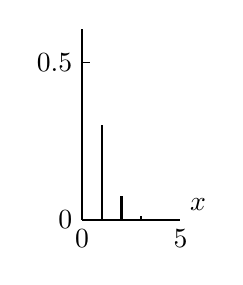
\begin{tikzpicture}[x={0.25cm},y={4cm}]
\foreach \x/\y in {0/0.607,1/0.303,2/0.076,3/0.013,4/0.0016}{\draw[thick](\x,0)--++(0,\y);}
\draw(0,0)node[left]{$0$}node[below]{$0$}--(5,0)node[below]{$5$}node[above right]{$x$};
\draw(0,0.5)node[left]{$0.5$}--++(0.4,0);
\end{tikzpicture}
\caption*{$\mu=0.5$}
\end{subfigure}%
\begin{subfigure}{0.2\textwidth}
\centering
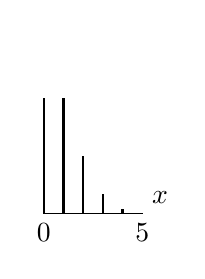
\begin{tikzpicture}[x={0.25cm},y={4cm}]
\foreach \x/\y in {0/0.368,1/0.368,2/0.184,3/0.061,4/0.015,5/0.003}{\draw[thick](\x,0)--++(0,\y);}
\draw(0,0)node[below]{$0$}--(5,0)node[below]{$5$}node[above right]{$x$};
\path(0,0)--++(0,0.59);
\end{tikzpicture}
\caption*{$\mu=1$}
\end{subfigure}%
\begin{subfigure}{0.2\textwidth}
\centering
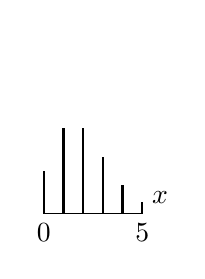
\begin{tikzpicture}[x={0.25cm},y={4cm}]
\foreach \x/\y in {0/0.135,1/0.27,2/0.27,3/0.18,4/0.09,5/0.036}{\draw[thick](\x,0)--++(0,\y);}
\draw(0,0)node[below]{$0$}--(5,0)node[below]{$5$}node[above right]{$x$};
\path(0,0)--++(0,0.59);
\end{tikzpicture}
\caption*{$\mu=2$}
\end{subfigure}%
\begin{subfigure}{0.4\textwidth}
\centering
\begin{tikzpicture}[x={0.25cm},y={4cm}]
\foreach \x/\y in {0/0.007,1/0.034,2/0.084,3/0.14,4/0.175,5/0.175,6/0.146,7/0.104,8/0.065,9/0.036,10/0.018,11/0.0082}{\draw[thick](\x,0)--++(0,\y);}
\draw(0,0)node[below]{$0$}--(11,0)node[below]{$11$}node[above right]{$x$};
\path(0,0)--++(0,0.59);
\end{tikzpicture}
\caption*{$\mu=5$}
\end{subfigure}%
\caption{مختلف \عددی{p} اور \عددی{n=5} کے لئے مساوات \حوالہ{مساوات_شماریات_پوئسن_تقسیم_الف} میں دی گئی پوئسن تقسیم}
\label{شکل_شماریات_پوئسن_مثالیں}
\end{figure}

\جزوحصہء{واپس رکھ کر اور واپس نہ رکھ کر نمونے کا حصول۔بیش ہندسی تقسیم}
واپس رکھ کر نمونہ حاصل کرنے میں ثنائی تقسیم (مثال \حوالہ{مثال_شماریات_واپس_رکھ_نہ_رکھ_کر_نمونہ}) اہم ہے۔ مثال کے طور پر ایک ڈبیا میں \عددی{N} پیچ ہیں جن میں سے \عددی{M} پیچ عیب دار ہیں۔اگر ہم ڈبے سے ایک پیچ بلا منصوبہ نکالیں تب عیب دار پیچ کے حصول کا احتمال
\begin{align*}
p=\frac{M}{N}
\end{align*}
ہو گا۔یوں واپس رکھ کر حاصل، \عددی{x} پیچوں کے نمونہ میں عیب دار پیچوں کی تعداد \عددی{x} ہونے کا احتمال (مساوات \حوالہ{مساوات_شماریات_ثنائی_تقسیم_ب})
\begin{align}\label{مساوات_شماریات_واپس_رکھ_کر_نمونہ}
f(x)=\binom{n}{x}\big(\frac{M}{N}\big)^x\big(1-\frac{M}{N}\big)^{n-x}\quad\quad (x=0,1,\cdots,n)
\end{align}
ہو گا۔واپس نہ رکھ کر حاصل نمونہ میں احتمال 
\begin{align}\label{مساوات_شماریات_بیش_ہندسی_تقسیم}
f(x)=\frac{\binom{M}{x}\binom{N-M}{n-x}}{\binom{N}{n}}\quad\quad (x=0,1,\cdots,n)
\end{align}
ہو گا۔مساوات \حوالہ{مساوات_شماریات_بیش_ہندسی_تقسیم} میں دی گئی تقسیم کو \اصطلاح{بیش ہندسی تقسیم}\فرہنگ{تقسیم!بیش ہندسی}\فرہنگ{بیش ہندسی!تقسیم}\حاشیہب{hypergeometric distribution}\فرہنگ{distribution!hypergeometric} کہتے\حاشیہد{چونکہ اس تقسیم کے معیار اثر کے پیدا کار تفاعل کو بیش ہندسی تفاعل کی صورت میں لکھا جا سکتا ہے۔} ہیں۔

مساوات \حوالہ{مساوات_شماریات_بیش_ہندسی_تقسیم} ثابت کرنے کی خاطر ہم دیکھتے ہیں کہ مساوات \حوالہ{مساوات_شماریات_مرتب_اجتماعات_ب} کے تحت 
\begin{itemize}
\item{(الف)}
\عددی{N} اشیاء میں سے \عددی{n} اشیاء کے انتخاب کے \عددی{\binom{N}{n}} مختلف طریقے ہیں،
\item{(ب)}
\عددی{M} میں سے \عددی{x} عیب دار کے انتخاب کے \عددی{\binom{M}{x}} مختلف طریقے ہیں،
\item{(پ)}
\عددی{N-M} میں سے \عددی{n-x} بے عیب کے انتخاب کے \عددی{\binom{N-M}{n-x}} مختلف طریقے ہیں،
\end{itemize}
اور (ب) میں ہر طریقہ کے ساتھ (پ) کا ہر طریقہ لے  کر، بغیر واپس رکھتے ہوئے \عددی{n} میں سے \عددی{x} عیب دار کی انتخاب کے کل طریقے حاصل ہوں گے۔چونکہ (الف) تمام وقوعات کا مجموعہ ہے اور ہم بلا منصوبہ انتخاب کرتے ہیں لہٰذا اس طرح کے ہر طریقہ کا احتمال \عددی{\tfrac{1}{\binom{N}{n}}} ہو گا۔یوں مساوات \حوالہ{مساوات_شماریات_بیش_ہندسی_تقسیم} ثابت ہوتا ہے۔

بیش ہندسی تقسیم کی اوسط (سوال \حوالہ{سوال_شماریات_اوسط_بیش_ہندسی_الف})
\begin{align}\label{مساوات_شماریات_اوسط_بیش_ہندسی_الف}
\mu=n\frac{M}{N}
\end{align}
اور تغیریت
\begin{align}
\sigma^{\,2}=\frac{nM(N-M)(N-n)}{N^2(N-1)}
\end{align}
ہے۔

%================
\ابتدا{مثال}\quad \موٹا{واپس رکھ کر اور نا رکھ کر نمونے کا حصول}\\
ایک ڈبہ میں \عددی{10} تصاویر ہیں جن میں سے \عددی{3} عیب دار ہیں۔ہم بلا منصوبہ \عددی{ 2} تصاویر ڈبے سے نکالتے ہیں۔بلا منصوبہ متغیر
\begin{align*}
X=\text{\RL{نمونہ میں عیب دار کی تعداد}}
\end{align*}
کا تفاعل احتمال تلاش کریں۔\\
حل:\quad
یہاں \عددی{N=10}، \عددی{M=3}، \عددی{N-M=7} اور \عددی{n=2} ہیں۔واپس رکھ کر نمونہ حاصل کرتے ہوئے مساوات \حوالہ{مساوات_شماریات_واپس_رکھ_کر_نمونہ} کے تحت
\begin{align*}
f(x)=\binom{2}{x}\big(\frac{3}{10}\big)^x\big(\frac{7}{10}\big)^{2-x},\quad f(0)=0.49,\quad f(1)=0.42,\quad f(2)=0.09
\end{align*}
حاصل ہوتا ہے۔ واپس نہ رکھ کر نمونہ حاصل کرتے ہوئے مساوات \حوالہ{مساوات_شماریات_بیش_ہندسی_تقسیم} سے
\begin{align*}
f(x)=\frac{\binom{3}{x}\binom{7}{2-x}}{\binom{10}{2}},\quad f(0)=f(1)=\frac{21}{45}\approx 0.47,\quad f(2)=\frac{3}{45}\approx 0.07
\end{align*}
حاصل ہوتا ہے۔
\انتہا{مثال}
%========================

اگر \عددی{n} کے لحاظ سے \عددی{N}، \عددی{M} اور \عددی{N-M} بہت بڑی مقدار ہوں تب واپس رکھتے ہوئے اور واپس نہ رکھتے ہوئے حاصل کردہ  نمونے تقریباً ایک جیسے ہوں گے لہٰذا ایسی صورت میں بیش ہندسی تقسیم کی جگہ \عددی{p=\tfrac{M}{N}} لیتے ہوئے ثنائی تقسیم استعمال کی جا سکتی ہے، جو نسبتاً سادہ تفاعل ہے۔

یوں بہت بڑی آبادی (\اصطلاح{لامتناہی آبادی}) سے،  واپس رکھتے ہوئے یا واپس نہ رکھتے ہوئے، نمونہ حاصل کرتے ہوئے ثنائی تقسیم استعمال کی جا سکتی ہے۔

%=====================
\حصہء{سوالات}
%=====================
\ابتدا{سوال}\quad
چار سکے ایک ساتھ  اچھالے جاتے ہیں۔بلا منصوبہ متغیر "\عددی{\text{\RL{تعداد خط}}=X}" کا تفاعل احتمال تلاش کریں؟ \عددی{0} خط، \عددی{1} خط، کم سے کم \عددی{1} خط اور زیادہ سے زیادہ \عددی{3}  خط کا احتمال حاصل کریں۔\\
جواب:\quad
$0.0625, 0.25, 0.9375,0.9375$
\انتہا{سوال}
%==========================
\ابتدا{سوال}\quad
نشانے پر تیر مارنے کا امکان \عددی{\SI{10}{\percent}} ہے۔ \عددی{10} تیر چلائے جاتے ہیں۔کم سے کم ایک بار نشانہ لگنے کا احتمال کیا ہو گا؟
\انتہا{سوال}
%========================
\ابتدا{سوال}\quad
\عددی{24} گھنٹوں کے پرکھ میں \عددی{p=\SI{1}{\percent}} امکان ہے کہ ایک خاص قسم کا بلب زائل ہو جائے گا۔ایسے \عددی{10} بلبوں کا ،کوئی بھی بلب خراب ہوئے بغیر، مسلسل \عددی{24} گھنٹے  روشنی دینے کا احتمال کیا ہو گا۔\\
جواب:\quad
$0.99^{10}\approx \SI{90.4}{\percent}$
\انتہا{سوال}
%=========================
\ابتدا{سوال}\شناخت{سوال_شماریات_ثنائی_ثبوت_الف}\quad
مسئلہ ثنائی استعمال کرتے ہوئے دکھائیں کہ ثنائی تقسیم کے  معیار اثر کا پیدا کار تفاعل (سوال \حوالہ{سوال_شماریات_معیار_اثر_پیدا_کار_تفاعل_الف}) درج ذیل ہے اور مساوات \حوالہ{مساوات_شماریات_ثنائی_تقسیم_پ} اور مساوات \حوالہ{مساوات_شماریات_ثنائی_تقسیم_ت} کو ثابت کریں۔
\begin{align*}
G(t)=\sum_{x=0}^{n}e^{tx}\binom{n}{x}p^xq^{n-x}=\sum_{x=0}^{n}\binom{n}{x}(pe^t)^xq^{n-x}=(pe^t+q)^n
\end{align*}  
\انتہا{سوال}
%===========================
\ابتدا{سوال}\شناخت{سوال_شماریات_پوئسن_ثبوت_الف}\quad
دکھائیں کہ پوئسن تقسیم کے  معیار اثر کا پیدا کار تفاعل  درج ذیل ہے اور مساوات \حوالہ{مساوات_شماریات_پوئسن_تقسیم_ب} کو ثابت کریں۔
\begin{align*}
G(t)=e^{-\mu}e^{\mu e^t}
\end{align*}  
\انتہا{سوال}
%===========================
\ابتدا{سوال}\quad
دکھائیں کہ \عددی{E([X-\mu]^3)=E(X^3)-3\mu E(X^2)+2\mu^3} ہو گا۔اس کو اور سوال \حوالہ{سوال_شماریات_پوئسن_ثبوت_الف} کو استعمال کرتے ہوئے  دکھائیں کہ پوئسن تقسیم کا ترچھاپن \عددی{\gamma=\tfrac{1}{\sqrt{\mu}}} ہے جو کہتا ہے کہ \عددی{\mu} کی بڑی قیمت کے لئے یہ تقسیم تقریباً تشاکلی ہے (شکل \حوالہ{شکل_شماریات_پوئسن_مثالیں})۔
\انتہا{سوال}
%============================
\ابتدا{سوال}\quad
دکھائیں کہ پوئسن تقسیم کا تفاعل تقسیم \عددی{F(\infty)=1} کو مطمئن کرتا ہے۔
\انتہا{سوال}
%==========================
\ابتدا{سوال}\quad
ایک ٹیلیفون تقسیم کار تختی اوسطاً \عددی{600} ٹیلیفون کے لئے کافی ہے۔ یہ ایک منٹ میں زیادہ سے زیادہ \عددی{10} نئے ٹیلیفون ملا سکتی ہے۔پوئسن تقسیم استعمال کرتے ہوئے اس بات کا احتمال تلاش کریں کہ کسی ایک منٹ میں یہ تقسیم کار تختی نا کافی ثابت ہو گا۔
\انتہا{سوال}
%=======================
\ابتدا{سوال}\quad
ایک کارخانے میں \عددی{\SI{50}{\ohm}} کے برقی مزاحمت پیدا کیے جاتے ہیں جن میں سے وہ مزاحمت بے عیب تصور کیے جاتے ہیں جن کی مزاحمت \عددی{\SI{45}{\ohm}} اور \عددی{\SI{55}{\ohm}} کے بیچ ہو۔عیب دار مزاحمت کا احتمال \عددی{\SI{0.2}{\percent}} ہے۔ان مزاحمتوں کو \عددی{100} کی کھیپ میں، ضمانت کے ساتھ فروخت کیا جاتا ہے۔تقسیم پوئسن استعمال کرتے ہوئے ایک کھیپ میں عیب دار مزاحمت نکلنے کا احتمال حاصل کریں۔\\
جواب:\quad
$1-e^{-0.2}=0.1813$
\انتہا{سوال}
%==========================
\ابتدا{سوال}\quad
فرض کریں کہ ایک مشین کے پیدا کردہ پیچوں میں سے  \عددی{\SI{3}{\percent}} عیب دار ہوتے ہیں۔ایک ڈبیا میں \عددی{50} پیچ بھرے جاتے ہیں۔تقسیم پوئسن استعمال کرتے ہوئے ایک ڈبیا میں \عددی{x} عیب دار پیچ نکلنے کا احتمال تلاش کریں۔
\انتہا{سوال}
%=============================
\ابتدا{سوال}\quad
ایک پل سے جمع کے دن صبح \عددی{8} تا \عددی{10} بجے  فی منٹ \عددی{X} گاڑیاں گزرتی ہیں۔فرض کریں کہ \عددی{X} کو پوئسن تقسیم ظاہر کرتی ہے جس کا اوسط \عددی{5} ہے۔کسی ایک منٹ میں \عددی{3} یا \عددی{3} سے کم گاڑیاں گزرنے کا احتمال تلاش کریں۔\\
جواب:\quad
$0.265$
\انتہا{سوال}
%================================
\ابتدا{سوال}\quad
ایک مقناطیسی پٹی کے \عددی{100} میٹر لمبائی میں اوسطاً \عددی{2} عیب پائے جاتے ہیں۔ \عددی{300} میٹر لمبی پٹی (الف) میں \عددی{x} عیب کا احتمال کیا ہو گا، (ب) بلا عیب ہونے کا احتمال کیا ہو گا؟ 
\انتہا{سوال}
%=============================
\ابتدا{سوال}\quad
گتے کے ڈبا میں \عددی{20} فتیلہ ہیں جن میں سے \عددی{5} عیب دار ہیں۔ اس ڈبا سے بلا منصوبہ \عددی{3} فتیلے بغیر واپس رکھے  بطور نمونہ نکالے جاتے ہیں۔اس نمونہ میں \عددی{x} عیب دار فتیلے ہونے کا احتمال کیا ہو گا؟
\انتہا{سوال}
%=======================
\ابتدا{سوال}\شناخت{سوال_شماریات_قلم_الف}\quad
ایک  تقسیم کار \عددی{100} قلم کے ڈبوں فروخت کرتا ہے۔وہ اس بات کی ضمانت دیتا ہے کہ کسی ایک ڈبے میں سے زیادہ سے زیادہ \عددی{\SI{10}{\percent}} قلم عیب دار ہوں گے۔ایک خریدار ہر ڈبے میں سے \عددی{10} قلم بغیر واپس رکھے نکال کر پرکھتا ہے۔کوئی بھی قلم عیب دار نہ ہونے کی صورت میں وہ ڈبا خرید لیتا ہے ورنہ وہ ڈبے کو نہیں خریدتا۔اس کا کیا احتمال ہے کہ ایک ڈبے میں \عددی{10} عیب دار قلم ہوں (لہٰذا یہ ضمانت پر پورا اترتا ہے) اور خریدار اس ڈبے کو نہ خریدے؟
\انتہا{سوال}
%=========================
\ابتدا{سوال}\quad
سوال \حوالہ{سوال_شماریات_قلم_الف} میں کیا احتمال ہے کہ ایک ڈبے میں \عددی{20} عیب دار قلم ہونے کے باوجود خریدار اسے خرید لیتا ہے؟
\انتہا{سوال}
%============================
\ابتدا{سوال}\quad
ایک کارخانے میں پیچوں کی پیداوار کی جاتی ہے۔ہر گھنٹہ بلا منصوبہ \عددی{n} پیچ کا نمونہ حاصل کر کے پرکھا جاتا ہے۔ایک یا ایک سے زیادہ عیب دار پیچ حاصل ہونے کی صورت میں کام روک کر مشینوں کی کارکردگی تسلی بخش بنائی جاتی ہے۔\عددی{n} کتنا ہو گا اگر  \عددی{\SI{10}{\percent}} عیب دار پیچ کی صورت میں \عددی{\SI{95}{\percent}} احتمال ہے کہ کام روکا جائے گا؟  
\انتہا{سوال}
%======================
\ابتدا{سوال}\quad
\عددی{1} سے لے کر \عددی{13} تک عدد کو علیحدہ علیحدہ کاغذ پر لکھا جاتا ہے۔ان میں سے بلا منصوبہ تین کاغذ نکالے جاتے ہیں جبکہ  ایک شخص  بغیر دیکھے  تینوں پر لکھے اعداد بتاتا ہے۔کیا احتمال ہے کہ وہ (الف) کوئی بھی درست عدد نہ بتائے، (ب) ایک عدد ٹھیک بتائے، (پ) دو عدد ٹھیک بتائے، (ت) تینوں اعداد ٹھیک بتائے؟  \\
جواب:\quad
$\tfrac{120}{286},\tfrac{135}{286},\tfrac{30}{286},\tfrac{1}{286}$ 
\انتہا{سوال}
%====================
\ابتدا{سوال}\شناخت{سوال_شماریات_اوسط_بیش_ہندسی_الف}\quad
مساوات \حوالہ{مساوات_شماریات_اوسط_بیش_ہندسی_الف} کو ثابت کریں۔
\انتہا{سوال}
%===========================
\ابتدا{سوال}\quad \موٹا{(متعدد رکنی تقسیم)}\quad
\عددی{k}  باہمی بلا شرکت وقوعات \عددی{A_1,\cdots,A_k} کے احتمال بالترتیب \عددی{p_1,\cdots,p_k} ہیں  جہاں \عددی{p_1+\cdots+p_k=1} ہے۔فرض کریں کہ \عددی{n} باہمی بلا شرکت کوشش کیے جاتے ہیں۔دکھائیں کہ ان میں \عددی{A_1} کی تعداد \عددی{x_1}، \نقطے، \عددی{A_k} کی تعداد \عددی{x_k} ہونے کا احتمال
\begin{align*}
f(x_1,\cdots,x_n)=\frac{n!}{x_1!\cdots x_k!}p_1^{x_1}\cdots p_k^{x_k}
\end{align*}
ہو گا جہاں \عددی{0\le x_j\le n}، \عددی{j=1,\cdots,k}، اور \عددی{x_1+\cdots+x_n=n} ہیں۔ایسی تقسیم جس کی تفاعل تقسیم درج بالا ہو کو \ترچھا{متعدد رکنی تقسیم}\فرہنگ{تقسیم!متعدد رکنی}\حاشیہب{multinomial distribution}\فرہنگ{distribution!multinomial} کہتے ہیں۔
\انتہا{سوال}
%=============================
\ابتدا{سوال}\quad
برقی مزاحمت کی پیداوار میں \عددی{\SI{3}{\percent}} کی مزاحمت \عددی{R<\SI{198}{\ohm}} اور \عددی{\SI{5}{\percent}} کی مزاحمت \عددی{R>\SI{201}{\ohm}} ہے۔بلا منصوبہ \عددی{20} مزاحمتوں کے نمونہ میں \عددی{R<\SI{198}{\ohm}} کے \عددی{x_1} اور \عددی{R>\SI{201}{\ohm}} کے \عددی{x_2} مزاحمت حاصل کرنے کا احتمال کیا ہو گا؟
\انتہا{سوال}
%===============================

\حصہ{عمومی تقسیم}
ایسی تقسیم جس کی کثافت
\begin{align}\label{مساوات_شماریات_عمومی_تقسیم_الف}
f(x)=\frac{1}{\sigma\sqrt{2\pi}}\,e^{-\frac{1}{2}(\frac{x-\mu}{\sigma})^2}\quad\quad\quad (\sigma>0)
\end{align}
ہو کو \اصطلاح{عمومی تقسیم}\فرہنگ{تقسیم!عمومی}\حاشیہب{normal distribution}\فرہنگ{distribution!normal} یا \ترچھا{گاوسی تقسیم}\فرہنگ{تقسیم!گاوسی}\فرہنگ{گاوس!گاوسی تقسیم}\حاشیہب{Gauss distribution}\فرہنگ{distribution!Gauss} کہتے ہیں۔اس طرح تقسیم والا بلا منصوبہ متغیر \اصطلاح{عمومی}\فرہنگ{عمومی}\حاشیہب{normal}\فرہنگ{normal} یا \اصطلاح{عمومی بانٹا ہوا}\فرہنگ{عمومی!بانٹا ہوا}\حاشیہب{normally distributed}\فرہنگ{normally distributed} کہلاتا ہے۔عملی دلچسپی کے بہت سارے بلا منصوبہ متغیرات عمومی یا تخمیناً عمومی ہیں اور یا ان کا تبادلہ با آسانی عمومی بلا منصوبہ متغیرات میں کیا جا سکتا ہے۔ اس کے علاوہ کئی پیچیدہ تقسیم کو تخمیناً عمومی تقسیم سے ظاہر کیا جا سکتا ہے۔شماریاتی پرکھ کے کئی ثبوت میں بھی یہ تقسیم کردار ادا کرتی ہے۔   


مساوات \حوالہ{مساوات_شماریات_عمومی_تقسیم_الف} میں تقسیم کی اوسط \عددی{\mu}  اور اس کا معیاری انحراف \عددی{\sigma}  ہے۔ \عددی{f(x)} کی منحنی \عددی{\mu} کے لحاظ سے تشاکلی ہے اور اس  کو \اصطلاح{قوس جرس}\فرہنگ{قوس!جرس}\فرہنگ{جرس!قوس}\حاشیہب{bell curve}\فرہنگ{bell curve} کہتے ہیں۔قوس جرس کو شکل \حوالہ{شکل_شماریات_عمومی_تقسیم} میں \عددی{\mu=0} اور \عددی{\sigma} کے کئی قیمتوں کے لئے دکھایا گیا ہے۔ \عددی{\mu>0} (\عددی{\mu<0}) کے لئے قوس کی شکل تبدیل نہیں ہوتی البتہ یہ \عددی{\abs{\mu}} اکائیاں دائیں (بائیں) منتقل ہوتا ہے۔\عددی{\sigma^{\,2}} کی قیمت جتنی کم ہو،\عددی{x=\mu} پر قوس کی چوٹی اتنی زیادہ بلند ہو گی اور چوٹی کے دونوں اطراف ڈھلوان اتنی زیادہ ہو گی (شکل \حوالہ{شکل_شماریات_عمومی_تقسیم}) جو تغیریت کے تصور کے عین مطابق ہے۔
\begin{figure}
\centering
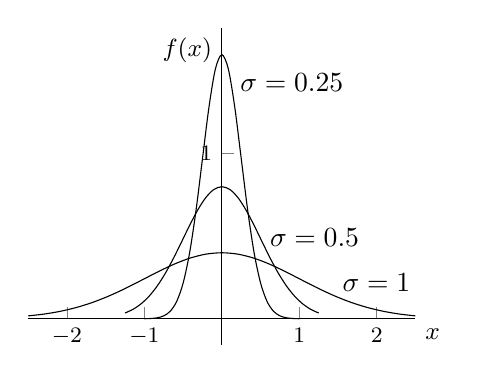
\begin{tikzpicture}
\begin{axis}[small,axis lines*=middle,ytick={1},yticklabels={$1$},xmin=-2.5,xmax=2.5,xlabel={$x$},x label style={at={(current axis.right of origin)},anchor=north west},ylabel={$f(x)$},y label style={rotate=-90},y label style={at={(current axis.above origin)},anchor=north east}]
\addplot[smooth,domain=-1:1] {1/(0.25*sqrt(2*pi))*e^(-0.5*((x-0)/0.25)^2)}node[pos=0.55,right]{$\sigma=0.25$};
\addplot[smooth,domain=-1.25:1.25] {1/(0.5*sqrt(2*pi))*e^(-0.5*((x-0)/0.5)^2)}node[pos=0.7,right]{$\sigma=0.5$};
\addplot[smooth,domain=-2.5:2.5] {1/(1*sqrt(2*pi))*e^(-0.5*((x-0)/1)^2)}node[pos=0.9,above,yshift={0.1cm}]{$\sigma=1$};
\end{axis}
\end{tikzpicture}
\caption{عمومی تقسیم (مساوات \حوالہ{مساوات_شماریات_عمومی_تقسیم_الف}) برائے \عددی{\mu=0} اور مختلف \عددی{\sigma}}
\label{شکل_شماریات_عمومی_تقسیم}
\end{figure}

مساوات \حوالہ{مساوات_شماریات_عمومی_تقسیم_الف} سے ہم دیکھتے ہیں کہ عمومی تقسیم کا تقسیمی تفاعل
\begin{align}\label{مساوات_شماریات_عمومی_تقسیم_ب}
F(x)=\frac{1}{\sigma\sqrt{2\pi}}\int_{-\infty}^{x}e^{-\frac{1}{2}(\frac{v-\mu}{\sigma})^2}\dif v
\end{align}
ہو گا۔یوں مساوات \حوالہ{مساوات_شماریات_استمراری_بلا_منصوبہ_متغیر_پ} سے درج ذیل حاصل ہو گا۔
\begin{align}\label{مساوات_شماریات_عمومی_تقسیم_پ}
P(a<X\le b)=F(b)-F(a)=\frac{1}{\sigma\sqrt{2\pi}}\int_{a}^{b}e^{-\frac{1}{2}(\frac{v-\mu}{\sigma})^2}\dif v
\end{align}

مساوات \حوالہ{مساوات_شماریات_عمومی_تقسیم_ب} کا تکمل بنیادی طریقوں سے حاصل کرنا ممکن نہیں ہے البتہ اس کو درج ذیل تکمل کی صورت میں لکھا جا سکتا ہے
\begin{align}\label{مساوات_شماریات_عمومی_تقسیم_ت}
\Phi(z)=\frac{1}{\sqrt{2\pi}}\int_{-\infty}^{z}e^{-\frac{u^2}{2}}\dif u
\end{align}
جو عمومی تقسیم کا وہ تفاعل ہے جس کی اوسط \عددی{0} اور تغیریت \عددی{1} ہے اور جس کو جدول بند کیا گیا ہے۔ یہ جدول ضمیمہ \حوالہ{ضمیمہ_جدول} میں پیش کیے گئے ہیں۔اگر \عددی{\tfrac{v-\mu}{\sigma}=u} لیا جائے تب \عددی{\tfrac{\dif u}{\dif v}=\tfrac{1}{\sigma}} اور \عددی{\dif v=\sigma \dif u} ہو گا اور ہمیں \عددی{-\infty} تا \عددی{z=\tfrac{x-\mu}{\sigma}} تکمل لینا ہو گا۔مساوات \حوالہ{مساوات_شماریات_عمومی_تقسیم_ب} سے یوں
\begin{align*}
F(x)=\frac{1}{\sigma\sqrt{2\pi}}\int_{-\infty}^{\frac{x-\mu}{\sigma}}e^{-\frac{u^2}{2}}\sigma \dif u
\end{align*}
حاصل ہو گا جس میں \عددی{\sigma} کٹ جاتا ہے اور جس کا دایاں ہاتھ مساوات \حوالہ{مساوات_شماریات_عمومی_تقسیم_ت} دیتا ہے جہاں  \عددی{z=\tfrac{x-\mu}{\sigma}} ہے یعنی:
\begin{align}\label{مساوات_شماریات_عمومی_تقسیم_ٹ}
F(x)=\Phi\big(\frac{x-\mu}{\sigma}\big)
\end{align}
اس سے اور مساوات \حوالہ{مساوات_شماریات_عمومی_تقسیم_پ} سے درج ذیل ایک اہم کلیہ  اخذ ہوتا ہے۔
\begin{align}\label{مساوات_شماریات_عمومی_تقسیم_ث}
P(a<X\le b)=F(b)-F(a)=\Phi\big(\frac{b-\mu}{\sigma}\big)-\Phi\big(\frac{a-\mu}{\sigma}\big)
\end{align}
بالخصوص \عددی{a=\mu-\sigma} اور \عددی{b=\mu+\sigma} کی صورت میں دایاں ہاتھ \عددی{\Phi(1)-\Phi(-1)} کے برابر ہے؛  
\عددی{a=\mu-2\sigma} اور \عددی{b=\mu+2\sigma} کی صورت میں دایاں ہاتھ \عددی{\Phi(2)-\Phi(-2)} کے برابر ہے، وغیرہ، وغیرہ۔تفاعل \عددی{\Phi(z)} کی قیمتیں جدول سے دیکھتے ہوئے درج ذیل حاصل ہوتا ہے۔
\begin{gather}
\begin{aligned}\label{مساوات_شماریات_عمومی_تقسیم_ج}
\text{(الف)}\quad P(\mu-\sigma<X\le \mu+\sigma)&\approx \SI{68}{\percent}\\
\text{(ب)}\quad P(\mu-2\sigma<X\le \mu+2\sigma)&\approx \SI{95.5}{\percent}\\
\text{(پ)}\quad P(\mu-3\sigma<X\le \mu+3\sigma)&\approx \SI{99.7}{\percent}
\end{aligned}
\end{gather}
یوں ہم توقع کرتے ہیں کہ بلا منصوبہ عمومی متغیر \عددی{X} کی بہت ساری قیمتیں درج ذیل طرح بانٹی گئی ہوں گی۔
\begin{itemize}
\item{(الف)}
تقریباً \عددی{\tfrac{2}{3}} قیمتیں \عددی{\mu-\sigma} اور \عددی{\mu+\sigma} کے بیچ ہوں گی،
\item{(ب)}
تقریباً \عددی{\SI{95}{\percent}} قیمتیں \عددی{\mu-2\sigma} اور \عددی{\mu+2\sigma} کے بیچ ہوں گی،
\item{(پ)}
تقریباً \عددی{99\tfrac{3}{4}\si{\percent}} قیمتیں \عددی{\mu-3\sigma} اور \عددی{\mu+3\sigma} کے بیچ ہوں گی
\end{itemize}
جس کو درج ذیل طریقہ سے بھی بیان کیا جا سکتا ہے۔

وہ قیمت جس کی \عددی{\mu} سے دوری \عددی{\sigma}  سے زیادہ ہو، \عددی{3} کوششوں میں تقریباً   \عددی{1} مرتبہ واقع ہو گی، جبکہ  وہ قیمت جس کی \عددی{\mu} سے دوری \عددی{2\sigma} یا \عددی{3\sigma}  سے زیادہ ہو، بالترتیب \عددی{20}  اور \عددی{400} کوششوں  میں تقریباً   \عددی{1} مرتبہ واقع ہو گی۔یوں عملی طور پر تمام قیمتیں \عددی{\mu-3\sigma} اور \عددی{\mu+3\sigma} کے بیچ پائی جائیں گی۔اس دو اعداد کو \اصطلاح{تین سگما حدود}\فرہنگ{تین سگما حدود}\حاشیہب{three-sigma limits}\فرہنگ{limit!three-sigma} کہتے ہیں۔

اسی طرح درج ذیل حاصل ہو گا۔
\begin{gather}
\begin{aligned}\label{مساوات_شماریات_چند_نتائج}
\text{(الف)}\quad P(\mu-1.96\sigma<X\le \mu+1.96\sigma)&=\SI{95}{\percent}\\
\text{(ب)}\quad P(\mu-2.58\sigma<X\le \mu+2.58\sigma)&=\SI{99}{\percent}\\
\text{(پ)}\quad P(\mu-3.29\sigma<X\le \mu+3.29\sigma)&=\SI{99.9}{\percent}
\end{aligned}
\end{gather}

درج ذیل مثال ضمیمہ \حوالہ{ضمیمہ_جدول} میں دیے گیے عمومی تقسیم کی جدول کا استعمال سمجھنے میں مدد دیں گی۔

%================
\ابتدا{مثال}
درج ذیل احتمال ضمیمہ \حوالہ{ضمیمہ_جدول} کی مدد سے تلاش کریں جہاں \عددی{X} عمومی ہے جس کی اوسط \عددی{0} اور تغیریت \عددی{1} ہے۔
\begin{align*}
\text{(الف)}\,\,P(X\le 2.44),\,\, \text{(ب)}\,\,P(X\le -1.16),\,\,\text{(پ)}\,\,P(X\ge 1),\,\, \text{(ت)}\,\,P(2\le X\le 10)
\end{align*}
حل:\quad ہم ضمیمہ \حوالہ{ضمیمہ_جدول} سے جوابات پڑھ کر لکھتے ہیں۔
\begin{align*}
\text{(الف)}\,\,0.9927,\quad \text{(ب)}\,\,0.1230, \quad \text{(پ)}\,\,1-P(X\le 1)=1-0.8413=0.1587,\\
\text{(ت)}\,\,\Phi(10)=1.0000 \,\text{(کیوں؟)}, \Phi(2)=0.9772,\Phi(10)-\Phi(2)=0.0228
\end{align*}
\انتہا{مثال}
%======================
\ابتدا{مثال}\quad
گزشتہ مثال کو دوبارہ حل کریں۔اس مرتبہ فرض کریں کہ \عددی{X}عمومی ہے جس کی اوسط \عددی{0.8} اور تغیریت \عددی{4} ہے۔\\
جواب:\quad
ضمیمہ \حوالہ{ضمیمہ_جدول} اور مساوات \حوالہ{مساوات_شماریات_عمومی_تقسیم_ث} استعمال کرتے ہوئے درج ذیل حاصل ہو گا۔
\begin{align*}
& \text{(الف)} \quad F(2.44)=\Phi(\frac{2.44-0.80}{2})=\Phi(0.82)=0.7939\\
& \text{(ب)} \quad F(-1.16)=\Phi(-0.98)=0.1635\\
& \text{(پ)} \quad 1-P(X\le 1)=1-F(1)=1-\Phi(0.1)=0.4602\\
& \text{(ت)} \quad F(10)-F(2)=\Phi(4.6)-\Phi(0.6)=1-0.7257=0.2743
\end{align*}
\انتہا{مثال}
%========================
\ابتدا{مثال}\quad
فرض کریں کہ \عددی{X} عمومی ہے جس کی اوسط \عددی{0} اور تغیریت \عددی{1} ہے۔ایسا مستقل \عددی{c} تلاش کریں جو درج ذیل کو مطمئن کرتا ہو۔
\begin{align*}
\text{(الف)}  \,\, P(X\ge c)&=\SI{10}{\percent},\quad \text{(ب)}  \,\,P(X\le c)=\SI{5}{\percent}\\
\text{(پ)}  \,\, P(0\le X\le c)&=\SI{45}{\percent},\quad \text{(ت)} \,\,P(-c\le X\le c)=\SI{99}{\percent}
\end{align*}
حل:\quad
ضمیمہ \حوالہ{ضمیمہ_جدول} سے  درج ذیل حاصل ہو گا۔
\begin{align*}
\text{(الف)}  \quad & 1-P(X\le c)=1-\Phi(c)=0.1, \Phi(c)=0.9, c=1.282,\\
\text{(ب)}  \quad & c=-1.645,\\
\text{(پ)} \quad &\Phi(c)-\Phi(0)=\Phi(c)-0.5=0.45,\Phi(c)=0.95,c=1.645,\\
\text{(ت)} \quad & c=2.576
\end{align*}
\انتہا{مثال}
%=========================
\ابتدا{سوال}\quad
فرض کریں کہ \عددی{X} عمومی ہے جس کی اوسط \عددی{-2} اور تغیریت \عددی{0.25} ہے۔ایسا \عددی{c} تلاش کریں جو درج ذیل کو مطمئن کرتا ہو۔
\begin{align*}
\text{(الف)} \,\,&P(X\ge c)=0.2,\quad \text{(ب)} \,\,P(-c\le X\le -1)=0.5\\
\text{(پ)} \,\,&P(-2-c\le X\le -2+c)=0.9,\quad \text{(ت)} \,\,P(-2-c\le X\le -2+c)=\SI{99.6}{\percent}
\end{align*}
حل:\quad
ضمیمہ \حوالہ{ضمیمہ_جدول} سے  درج ذیل حاصل ہو گا۔
\begin{align*}
&\text{(الف)}  \,\, 1-P(X\le c)=1-\Phi(\frac{c+2}{0.5})=0.2,\\
&\quad \quad \Phi(2c+4)=0.8, 2c+4=0.842,c=-1.579\\
&\text{(ب)}  \,\, \Phi(\frac{-1+2}{0.5})-\Phi(\frac{-c+2}{0.5})=0.9772-\Phi(4-2c)=0.5,\\
&\quad \quad \Phi(4-2c)=0.4772, 4-2c=-0.057, c=2.03\\
&\text{(پ)}  \,\,\Phi(\frac{-2+c+2}{0.5})-\Phi(\frac{-2-c+2}{0.5})\\
&\quad \quad =\Phi(2c)-\Phi(-2c)=0.9,2c=1.645,c=0.823\\
&\text{(ت)}  \,\,\Phi(2c)-\Phi(-2c)=\SI{99.6}{\percent}, 2c=2.878,c=1.439
\end{align*}
\انتہا{سوال}
%=========================
\ابتدا{مثال}\شناخت{مثال_شماریات_لوہے_کی_چادر}\quad
ایک کارخانے میں ایک خاص موٹائی کی لوہے کی چادریں بنائی جاتی ہیں۔یہ کام خود کار مشین کرتے ہیں۔ خام مال میں فرق اور درجہ حرارت، لرزش وغیرہ کی بنا  مشینوں کا رویہ اور استعمال آلات میں معمولی تبدیلیاں رو نما ہوتی ہیں جنہیں قبل از وقت جاننا ممکن نہیں ہوتا ہے۔ان وجوہات کی بنا چادریں ایک دوسرے سے مختلف ہوتی ہیں۔یوں ہم چادر کی موٹائی \عددی{X} (ملی میٹر) کو بلا منصوبہ متغیر تصور کر سکتے ہیں۔ہم فرض کرتے ہیں کہ یہ متغیر عمومی ہے جس کی اوسط \عددی{\mu=\SI{10}{\milli\meter}} اور معیاری انحراف \عددی{\sigma=\SI{0.02}{\milli\meter}} ہے۔ہم عیب دار چادروں کی تعداد جاننا چاہیں گے۔عیب دار چادر وہ چادر ہے  جس کی موٹائی (الف) \عددی{\SI{9.97}{\milli\meter}} سے کم ہو، (ب) \عددی{\SI{10.05}{\milli\meter}} سے زیادہ ہو، (پ) کا اوسط (\عددی{\SI{10}{\milli\meter}}) سے انحراف \عددی{\SI{0.03}{\milli\meter}} سے زیادہ ہو۔ (ت) ہم اعداد \عددی{10-c} اور \عددی{10+c} منتخب کرنا چاہتے ہیں کہ عیب دار چادروں کی تعداد \عددی{\SI{5}{\percent}} سے زیادہ نہ ہو۔(ٹ) جزو-ت میں
 \عددی{\mu=\SI{10.01}{\milli\meter}} کرنے سے عیب دار کی فی صد تعداد پر کیا اثر پڑے گا؟

حل:\quad
 ضمیمہ \حوالہ{ضمیمہ_جدول} استعمال کرتے ہوئے درج ذیل نتائج حاصل ہوتے ہیں۔
\begin{align*}
\text{(الف)}\quad P(X\le 9.97)=\Phi(\frac{9.97-10.00}{0.02})=\Phi(-1.5)=0.0668\approx \SI{6.7}{\percent}\\
\text{(ب)} \quad P(X\ge 10.05)=1-P(X\le 10.05)=1-\Phi(\frac{10.05-10.00}{0.02})\\
=1-\Phi(2.5)=1-0.9938\approx \SI{0.6}{\percent}\\
\text{(پ)}  \quad P(9.97\le X\le 10.03)=\Phi(\frac{10.03-10.00}{0.02})-\Phi(\frac{9.97-10.00}{0.02})\\
=\Phi(1.5)-\Phi(-1.5)=0.8664; \implies 1-0.8664\approx \SI{13}{\percent}
\end{align*}
(ت) مساوات \حوالہ{مساوات_شماریات_چند_نتائج}-الف سے
\begin{align*}
c=1.96\sigma=0.039
\end{align*}
یوں جواب \عددی{\SI{9.961}{\milli\meter}} اور \عددی{\SI{10.039}{\milli\meter}} ہے۔\\
\begin{align*}
\text{(ٹ)} \quad P(9.961\le X\le 10.039)=\Phi(\frac{10.039-10.010}{0.02})-\Phi(\frac{9.961-10.010}{0.02})\\
=\Phi(1.45)-\Phi(-2.45)=0.9265-0.0071\approx \SI{92}{\percent}
\end{align*}
لہٰذا جواب \عددی{\SI{8}{\percent}} ہو گا۔آپ نے دیکھا کہ مشین میں معمولی تبدیلی سے عیب دار چادروں کی تعداد میں بہت زیادہ اضافہ پیدا ہوتا ہے۔

\انتہا{مثال}
%============================

بلا منصوبہ عمومی متغیر سے خطی تبادل کے ذریعہ بلا منصوبہ عمومی متغیر  ہی حاصل ہو گا۔مساوات \حوالہ{مساوات_شماریات_عمومی_تقسیم_ٹ} سے آپ یقیناً درج ذیل حاصل کر پائیں گے۔

%================
\ابتدا{مسئلہ}\شناخت{مسئلہ_شماریات_خطی_تبادل_دوسرا}\quad \موٹا{(خطی تبادل)}\\
اگر \عددی{X} عمومی ہو اور اس کی اوسط \عددی{\mu} اور تغیریت \عددی{\sigma^{\,2}} ہو تب \عددی{X^*=c_1X+c_2\,\, (c_1\ne 0)} عمومی ہو گا جس کی اوسط \عددی{\mu^*=c_1\mu+c_2} اور تغیریت \عددی{\sigma^{*2}=c_1^2\sigma^{\,2}} ہو گی۔
\انتہا{مسئلہ}
%====================== 

بڑی \عددی{n} کی صورت میں ثنائی تقسیم کو تخمیناً عمومی تقسیم سے ظاہر کیا جا سکتا ہے۔بڑی \عددی{n} کی صورت میں تفاعل تقسیم
\begin{align}\label{مساوات_شماریات_ثنائی_مشکل}
f(x)=\binom{n}{x}p^xq^{n-x}\quad\quad\quad (x=0,1,\cdots,n)
\end{align} 
کے ثنائی عددی سر اور طاقت سادہ نہیں رہتے اور ان سے چھٹکارا  حاصل کرنے میں بہتری ہے۔

%============
\ابتدا{مسئلہ}\quad \موٹا{(ڈی موے ور اور لاپلاس کا تحدیدی مسئلہ)}\\
بڑی \عددی{n} کے لئے
\begin{align*}
f(x)\sim f^*(x)\quad\quad\quad (x=0,1,\cdots,n)
\end{align*}
ہو گا جہاں \عددی{f} کو مساوات \حوالہ{مساوات_شماریات_ثنائی_مشکل} میں پیش کیا گیا ہے جبکہ
\begin{align}\label{مساوات_شماریات_ڈی_موے_الف}
f^*(x)=\frac{1}{\sqrt{2\pi}\sqrt{npq}}\,e^{-\frac{z^2}{2}},\quad z=\frac{x-np}{\sqrt{npq}}
\end{align}
عمومی تقسیم کی کثافت ہے جس کی اوسط \عددی{\mu=np} اور تغیریت \عددی{\sigma^{\,2}=npq} ہے (جو ثنائی تقسیم کی اوسط اور تغیریت ہیں) اور علامت \عددی{\sim} (\ترچھا{متقاربی برابر}) کا مطلب ہے کہ جیسے جیسے \عددی{n} لامتناہی کے قریب تر ہوتا جائے  ویسے ویسے دونوں اطراف کی نسبت \عددی{1} کے قریب تر ہوتی جائے گی۔ مزید کسی بھی غیر منفی اعداد صحیح \عددی{a} اور \عددی{b\,(>a)} کے لئے درج ذیل ہو گا۔
\begin{gather}
\begin{aligned}\label{مساوات_شماریات_ڈی_موے_ب}
P(a\le X\le b)=\sum_{x=a}^{b}\binom{n}{x}p^xq^{n-x}\sim \Phi(\beta)-\Phi(\alpha),\\
\alpha=\frac{a-np-0.5}{\sqrt{npq}},\quad \beta=\frac{b-np+0.5}{\sqrt{npq}}
\end{aligned}
\end{gather}
\انتہا{مسئلہ}
%=====================
اس مسئلے کا ثبوت اس کتاب میں پیش نہیں کیا جائے گا۔ اس مسئلے کے ثبوت  سے ظاہر ہوتا ہے کہ غیر مسلسل سے استمراری صورت میں تبادلے کی بنا اصلاح کی ضرورت پیش آتی ہے جو اجزاء \عددی{0.5}، \عددی{\alpha} اور \عددی{\beta} کی صورت میں نظر آتا ہے۔

%==================
\حصہء{سوالات}
%===============
\ابتدا{سوال}\quad
دکھائیں کہ مساوات \حوالہ{مساوات_شماریات_عمومی_تقسیم_الف} کے\اصطلاح{نقاط تصریف}\فرہنگ{نقطہ!تصریف}\حاشیہب{inflextion points}\فرہنگ{inflection point} \عددی{x=\mu-\sigma} اور \عددی{x=\mu+\sigma} پر پائے جاتے ہیں۔ نقطہ تصریف سے مراد وہ نقطہ ہے جس پر منحنی کی شکل محدب سے مجوف یا مجوف سے محدب ہوتی ہو۔
\انتہا{سوال}
%=======================
\ابتدا{سوال}\quad
دکھائیں \عددی{\Phi(-z)=1-\Phi(z)}
\انتہا{سوال}
%=======================
\ابتدا{سوال}\quad
\عددی{X} عمومی متغیر ہے جس کی اوسط \عددی{80} اور تغیریت \عددی{9} ہے۔\عددی{P(X>83)}، \عددی{P(X<81)}، \عددی{P(X<80)} اور \عددی{P(78<X<82)} تلاش کریں۔\\
جواب:\quad
$0.1587,0.6306,0.5,0.4950$
\انتہا{سوال}
%=========================
\ابتدا{سوال}\quad
\عددی{X} عمومی متغیر ہے جس کی اوسط \عددی{105} اور تغیریت \عددی{25} ہے۔\عددی{P(X\le 112.5)}، \عددی{P(X>100)} اور \عددی{P(110.5<X<111.25)} تلاش کریں۔\\
جواب:\quad
\انتہا{سوال}
%==================
\ابتدا{سوال}\quad
\عددی{X} عمومی ہے جس کی اوسط \عددی{14} اور تغیریت \عددی{4} ہے۔ایسا \عددی{c}  کہ \عددی{P(X\le c)=\SI{95}{\percent}}، \عددی{P(X\le c)=\SI{5}{\percent}}، \عددی{P(-c\le X\le c)=\SI{99}{\percent}} ہو تلاش کریں۔\\
جواب:\quad
$17.29,-17.29,19.152$
\انتہا{سوال}
%====================
\ابتدا{سوال}\quad
\عددی{X} عمومی ہے جس کی اوسط \عددی{3.6} اور تغیریت \عددی{0.01} ہے۔ایسا \عددی{c} تلاش کریں کہ \عددی{P(X\le c)=\SI{50}{\percent}}،
 \عددی{P(X> c)=\SI{10}{\percent}}، \عددی{P(-c< X\le c)=\SI{99.9}{\percent}} ہوں۔
\انتہا{سوال}
%======================
\ابتدا{سوال}\quad
گاڑی کی ایک مخصوص بیٹری کی زندگی \عددی{X} عمومی متغیر ہے جس کی اوسط \عددی{4} سال اور معیاری انحراف \عددی{1} سال ہے۔ صنعت گر بیٹری کی تین سال کی ضمانت دیتا ہے۔اس کو ضمانت کی بنا کتنی فی صد بیٹریاں مہیا کرنی ہوں گی؟\\
جواب:\quad
$\SI{16}{\percent}$
\انتہا{سوال}
%======================
\ابتدا{سوال}\quad
ایک سکہ \عددی{4040} مرتبہ اچھالا جاتا ہے۔\عددی{2048} شیر حاصل ہونے کا احتمال کیا ہو گا؟
\انتہا{سوال}
%=======================
\ابتدا{سوال}\quad
ایک صنعت کار کاغذ بناتا ہے جس کی کمیت عمومی متغیر ہے جس کی اوسط \عددی{\mu=\SI{1.950}{\gram}} اور معیاری انحراف \عددی{\sigma=\SI{0.025}{\gram}} ہے۔کاغذ کو \عددی{1000} کی جتھوں میں فروخت کیا جاتا ہے۔ایک جتھا میں کتنے کاغذ \عددی{\SI{2}{\gram}} سے زیادہ بھاری ہوں گے؟\\
جواب:\quad تقریباً \عددی{22}
\انتہا{سوال}
%=========================
\ابتدا{سوال}\quad
مثال \حوالہ{مثال_شماریات_لوہے_کی_چادر} کے جزو-پ میں عیب دار چادروں کی تعداد \عددی{\SI{6}{\percent}} کے لئے \عددی{\sigma} کتنا ہو گا؟ 
\انتہا{سوال}
%=======================
\ابتدا{سوال}\quad
برقی مزاحمت بنانے والا صنعت کار تجربہ سے جانتا ہے کہ اس کے بنائے گئے مزاحمت کی قیمت عمومی متغیر ہے جس کی اوسط \عددی{\mu=\SI{150}{\ohm}} اور معیاری انحراف \عددی{\sigma=\SI{5}{\ohm}} ہے۔کتنے فی صد کی مزاحمت \عددی{\SI{148}{\ohm}} اور \عددی{\SI{152}{\ohm}} کے بیچ ہو گی؟  کتنے فی صد کی مزاحمت \عددی{\SI{140}{\ohm}} اور \عددی{\SI{160}{\ohm}} کے بیچ ہو گی؟  \\
جواب:\quad
$\SI{31.1}{\percent},\SI{95.5}{\percent}$
\انتہا{سوال}
%=======================
\ابتدا{سوال}\quad
ایک پلاسٹک اینٹ کی \ترچھا{طاقت توڑ}\فرہنگ{طاقت!توڑ}\حاشیہب{breaking strength}\فرہنگ{strength!breaking} \عددی{X} (کلوگرام) عمومی متغیر ہے جس کی اوسط \عددی{\SI{1250}{\kilo\gram}} اور معیاری انحراف \عددی{\SI{55}{\kilo\gram}} ہے۔وہ کمیت تلاش کریں جس پر پلاسٹک ٹوٹنے کا انحراف \عددی{\SI{5}{\percent}} سے زیادہ نہ ہو۔ 
\انتہا{سوال}
%=====================
\ابتدا{سوال}\quad
ایک صارف کو \عددی{0.280\mp\SI{0.002}{\centi\meter}} قطر کے قابلے درکار ہیں۔ایک صنعت کار کے بنائے گئے  قابلوں کی  \عددی{\mu=\SI{0.279}{\centi\meter}} اور \عددی{\sigma=\SI{0.001}{\centi\meter}} ہے اور ان کی تقسیم عمومی ہے۔اس صنعت کار کے کتنے فی صد قابلے صارف کی تخصیص پر پورا اترتے ہیں؟\\
جواب:\quad
$\SI{84}{\percent}$
\انتہا{سوال}
%========================
\ابتدا{سوال}\quad
ایک فروش کار  \عددی{1000} بلب  گتے کے ایک ڈبے میں بیچتا ہے۔  \عددی{p=\SI{1}{\percent}} لیتے ہوئے مساوات \حوالہ{مساوات_شماریات_ڈی_موے_ب} کی مدد سے اس بات کا احتمال تلاش کریں کہ ایک ڈبے میں \عددی{\SI{1}{\percent}} سے زیادہ بلب خراب نہیں ہوں گے۔
\انتہا{سوال}
%===========================
\ابتدا{سوال}\quad
جدول عمومی استعمال کرتے ہوئے مساوات \حوالہ{مساوات_شماریات_چند_نتائج} میں دیے گئے نتائج حاصل کریں۔
\انتہا{سوال}
%==========================
\ابتدا{سوال}\quad
مسئلہ \حوالہ{مسئلہ_شماریات_خطی_تبادل_دوسرا} ثابت کریں۔
\انتہا{سوال}
%=============================
\ابتدا{سوال}\quad
اگر \عددی{X} عمومی ہو جس کی اوسط \عددی{\mu} اور تغیریت \عددی{\sigma^2} ہے تب \عددی{-X} کی تقسیم کیا ہو گی؟\\
جواب:\quad
\عددی{-X} بھی عمومی ہو گا۔اس کی اوسط \عددی{-\mu} اور تغیریت \عددی{\sigma^2} ہو گی۔
\انتہا{سوال}
%=========================
\ابتدا{سوال}\quad \موٹا{(بڑے اعداد کے لئے برنولی کا قاعدہ)}\\
فرض کریں کہ ایک تجربہ میں وقوعہ \عددی{A} کا احتمال \عددی{p\, (0<p<1)} ہے، اور فرض کریں کہ \عددی{n} بلا منصوبہ کوششوں میں \عددی{A} واقع ہونے کی تعداد \عددی{X} ہے۔دکھائیں کہ کسی بھی \عددی{\epsilon>0} کے \عددی{n\to\infty} کرتے ہوئے  درج ذیل ذیل ہو گا۔
\begin{align}
P\big(\abs{\frac{X}{n}-p}<\epsilon\big)\to  1\quad \quad \quad (n\to \infty)
\end{align}
\انتہا{سوال}
%============================
\ابتدا{سوال}\quad
\عددی{\Phi^2(\infty)} میں قطبی محدد (\عددی{u=r\cos \theta, v=r\sin \theta}) متعارف کرتے ہوئے درج ذیل ثابت کریں۔
\begin{align}\label{مساوات_شماریات_سوال_مساوات}
\Phi(\infty)=\frac{1}{\sqrt{2\pi}}\int_{-\infty}^{\infty} e^{-\tfrac{u^2}{2}}\dif u=1
\end{align}
جواب:\quad
\begin{align*}
\Phi^2(\infty)=\frac{1}{2\pi}\int_{-\infty}^{\infty}\int_{-\infty}^{\infty}e^{-\tfrac{u^2}{2}}e^{-\tfrac{v^2}{2}}\dif u\dif v=\frac{1}{2\pi}\int_{0}^{2\pi}\int_{0}^{\infty} e^{-\tfrac{r^2}{2}}r\dif r \dif \theta=1
\end{align*}
\انتہا{سوال}
%=======================
\ابتدا{سوال}\quad
مساوات \حوالہ{مساوات_شماریات_سوال_مساوات} اور تکمل بالحصص استعمال کرتے ہوئے دکھائیں کہ مساوات \حوالہ{مساوات_شماریات_عمومی_تقسیم_الف} میں \عددی{\sigma} معیاری تقسیم کا  معیاری انحراف ہے۔
\انتہا{سوال}
%======================


